\chapter{Propositional Calculus}
\section{Introduction}
\href{https://en.wikipedia.org/wiki/Propositional_calculus}{Propositional calculus}
(also known as \blue{propositional logic}) deals with the connection of
\blue{propositions}\index{propositions} 
(a.k.a. \blue{simple statements}) through 
\blue{logical connectives}.  Here, logical connectives are words like ``\blue{and}'', ``\blue{or}'',
``\blue{not}'', ``\blue{if $\cdots$, then}'', and ``\blue{exactly if}''.  To
start with, we define the notion of an \blue{atomic propositions}: An
\blue{atomic proposition}\index{atomic proposition} is a sentence  that 
\begin{itemize}
\item expresses a fact that is either true or false and
\item that does not contain any logical connectives.

      This last property is the reason for calling the proposition \blue{atomic}.
\end{itemize}
Examples of atomic propositions are the following:
\begin{enumerate}
\item ``\textsl{The sun is shining}''
\item ``\textsl{It is raining.}''
\item ``\textsl{There is a rainbow in the sky.}''
\end{enumerate}
Atomic propositions can be combined by means of logical connectives
into \blue{composite propositions}\index{composite propositions}.  An example for a
composite propositions would be
\\[0.2cm] 
\hspace*{1.3cm}
\textsl{\blue{If} the sun is shining \blue{and} it is raining, \blue{then} there is a rainbow in the sky.} 
\hspace*{\fill} (1)
\\[0.2cm]
This statement is composed of the three atomic propositions
\begin{itemize}
\item ``\textsl{The sun is shining.}'', 
\item ``\textsl{It is raining.}'', and
\item ``\textsl{There is a rainbow in the sky.}''
\end{itemize}
using the logical connectives ``\textsl{and}'' and ``\textsl{if $\cdots$, then}''.
Propositional calculus investigates how the truth value of composite statements is
calculated from the truth values of the propositions.  Furthermore, it investigates
how new statements can be \blue{derived} from given statements. 

In order to analyze the structure of complex statements we introduce
\blue{propositional variables}\index{propositional variables}.
These propositional variables are just names that denote atomic propositions.
Furthermore, we introduce symbols serving as mathematical operators for the logical connectives
``\blue{not}'', ``\blue{and}'', ``\blue{or}'', ``\blue{if, $\cdots$ then}'', and 
``\blue{if and only if}''.
\begin{enumerate}
\item $\neg a$ \index{$\neg a$}\quad\quad\ is read as \quad \blue{not} $a$ 
      \vspace*{-0.2cm}

\item $a \wedge b$ \index{$a \wedge b$}\,\quad\ is read as \quad $a$ \blue{and} $b$
      \vspace*{-0.2cm}

\item $a \vee b$ \index{$a \vee b$}\,\quad\ is read as \quad $a$ \blue{or} $b$
      \vspace*{-0.2cm}

\item $a \rightarrow b$ \index{$a \rightarrow b$}  \quad is read as \quad \blue{if} $a$, \blue{then} $b$
      \vspace*{-0.2cm}

\item $a \leftrightarrow b$ \index{$a \leftrightarrow b$} \quad is read as \quad  $a$ \blue{if and only if} $b$
\end{enumerate}
\blue{Propositional formulas} are built from propositional variables using the propositional operators shown
above and can have an arbitrary complexity.
Using propositional operators, the statement (1) can be written as follows:
 \\[0.2cm]
\hspace*{1.3cm}
$\texttt{sunny} \wedge \texttt{raining} \rightarrow \texttt{rainBow}$.
\\[0.2cm]
Here, we have used  $\texttt{sunny}$, $\texttt{rainy}$ and $\texttt{rainBow}$ as propositional variables.

Some propositional formulas are always true, no matter how the propositional variables are interpreted.
For example, the propositional formula 
\\[0.2cm]
\hspace*{1.3cm}
$p \vee \neg p$
\\[0.2cm]
is always true, it does not matter whether the proposition denoted by $p$ is true or false.  A propositional
formula that is always true is known as a  \blue{tautology}\index{tautology}.  There are also propositional
formulas that are never true.  For example, the propositional formula
\\[0.2cm]
\hspace*{1.3cm}
$p \wedge \neg p$
\\[0.2cm]
is always false.  A propositional formula is called \blue{satisfiable}\index{satisfiable}, if there is at least
one way to assign truth values to the variables such that the formula is true.  Otherwise the formula is called
\blue{unsatisfiable}\index{unsatisfiable}.  In this lecture we will discuss a number of different algorithms to
check whether a formula is satisfiable.  These algorithms are very important in a number of industrial
applications.  For example, a very important application is the design of digital circuits.
Furthermore, a number of \href{https://en.wikipedia.org/wiki/Category:Logic_puzzles}{logic puzzles} can be
translated into propositional formulas and finding a solution to these 
puzzles amounts to checking the satisfiable of these formulas.  For example, we will solve the
\href{https://en.wikipedia.org/wiki/Eight_queens_puzzle}{eight queens puzzle} in this way.

The rest of this chapter is structured as follows:

\begin{enumerate}
\item We list several applications of propositional logic.
\item We define the notion of propositional formulas, i.e.~we define the set of strings that are
      propositional formulas.

      This is known as the \blue{syntax} of propositional formulas.
\item Next, we discuss the \blue{evaluation} of propositional formulas and implement the evaluation in \textsl{Python}.

      This is known as the \blue{semantics} of propositional formulas.
\item Then we formally define the notions \blue{tautology} and \blue{satisfiability} for propositional formulas.   
\item We discuss algebraic manipulations of propositional formulas and introduce the 
      \blue{conjunctive normal form}.

      Some algorithms discussed later require that the propositional formulas have conjunctive normal form.
\item After that we discuss the concept of a \blue{logical derivation}.  The purpose of a logical derivation is to
      derive new formulas from a given set of formulas.
\item Finally, we discuss the \href{https://en.wikipedia.org/wiki/Davis–Putnam_algorithm}{Davis-Putnam
      algorithm} for checking the satisfiability of a set of  propositional formulas.  As an application, we
      solve the \href{https://en.wikipedia.org/wiki/Eight_queens_puzzle}{eight queens puzzle} using this algorithm.
\end{enumerate}

\section{Applications of Propositional Logic}
Propositional logic is not only the basis of first order logic, but it also has important practical
applications.  As there are many different applications of propositional logic, I will only list those
applications which I have seen myself during the years when I did work in industry.
\begin{enumerate}
\item \href{https://en.wikipedia.org/wiki/Electronic_design_automation}{Analysis and design of electronic circuits}.

      Modern digital circuits are comprised of hundreds of millions of logical gates.\footnote{The web page
      \href{https://en.wikipedia.org/wiki/Transistor_count}{\texttt{https://en.wikipedia.org/wiki/Transistor\_count}}
      gives an overview of the complexity of modern processors.}
      A logical gate  is a building block, that represents a logical connective such as ``\blue{and}'',
      ``\blue{or}'', ``\blue{not}'' as an electronic circuit.

      The complexity of modern digital circuits would be unmanageable without
      the use of computer-aided verification methods.  The methods used are applications of propositional logic. 
      A very concrete application is \blue{circuit comparison}.  Here two
      digital circuits are represented as propositional formulas.
      Afterwards it is tried to show the equivalence of these formulas by means of propositional logic.
      Software tools, which are used for the verification of digital
      circuits sometimes cost more than $100\,000\,\symbol{36}$.
      For example, the company Magma offers the \blue{equivalence checker}
      \href{https://www.eetimes.com/document.asp?doc_id=1217672}{Quartz Formal} at a price
      of $150\,000\,
      \symbol{36}$ per license.  Such a license is then valid for three years.


\item Controlling the signals and switches of railroad stations.

      At a large railway station, there are several hundred switches and signals that have to be 
      reset all the time to provide routes for the trains.
      For safety reasons, different routes must not cross each other.  
      The individual routes are described by so-called \blue{closure plans}.
      The correctness of these closure plans can be analyzed via propositional formulas.
\item A number of \blue{logical puzzles} can be coded as propositional formulas and can then be solved with the
      algorithm of Davis and Putnam.
      For example, we will discuss the 
      \href{https://en.wikipedia.org/wiki/Eight_queens_puzzle}{eight queens puzzle} in this lecture.
      This puzzle asks to place eight queens on a chess board such that no two queens can attack each other.
\end{enumerate}

\section{The Formal Definition of Propositional Formulas}
In this section we first cover the \blue{syntax} of propositional formulas.  After that, we discuss their
\blue{semantics}. The  \blue{syntax}\index{syntax} defines the way in which we represent formulas as strings
and how we can combine formulas into a \blue{proof}.  The  \blue{semantics}\index{semantics} of propositional
logic is concerned with the  \blue{meaning} of propositional formulas.
We will first define the semantics of propositional logic with the help of set theory.
Then, we implement this semantics in \textsl{Python}.

\subsection{The Syntax of Propositional Formulas}
We define propositional formulas as strings.  To this end we assume a set  $\mathcal{P}$ \index{$\mathcal{P}$, set of propositional variables} 
of so called \blue{propositional variables}\index{propositional variables} as given. 
Typically, $\mathcal{P}$ is the set of all lower case Latin characters, which additionally may be indexed.
For example, we will use 
\\[0.2cm]
\hspace*{1.3cm}
$p$, $q$, $r$, $p_1$, $p_2$, $p_3$
\\[0.2cm]
as propositional variables.  Then, propositional formulas are strings that are formed from the alphabet
$$ 
  \mathcal{A} := \mathcal{P} \cup \bigl\{ \verum, \falsum, \neg, \vee, \wedge,
   \rightarrow, \leftrightarrow, (, ) \bigr\}.
$$
We define the set $\mathcal{F}$ of 
\blue{propositional formulas}\index{propositional formulas}
\index{$\mathcal{F}$: set of propositional formulas}
by induction:
\begin{enumerate}
\item $\verum \in \mathcal{F}$ and $\falsum \in \mathcal{F}$.

      Here $\verum$ \index{$\verum$, Verum} \index{Verum} denotes the formula that is always true, while $\falsum$
      \index{$\falsum$, Falsum} \index{Falsum} denotes the formula that is always false.
      The formula $\verum$ is called
      ``\blue{verum}''\footnote{``\href{https://translate.google.com/?sl=la&tl=en&text=falsum&op=translate&hl=en}{Verum}''
        is the Latin word for ``true''.},  while $\falsum$ is called 
      ``\blue{falsum}''\footnote{``\href{https://translate.google.com/?sl=la&tl=en&text=falsum&op=translate&hl=en}{Falsum}''
        is the Latin word for ``false''.}.  
\item If $p \in \mathcal{P}$, then  $p \in \mathcal{F}$.

      Every propositional variable is also a propositional formula.
\item If $f \in \mathcal{F}$, then  $\neg f \in \mathcal{F}$.

      The formula  $\neg f$ \index{$\neg f$} (read: \blue{not $f$}) is called the \blue{negation}\index{negation} of $f$.
\item If $f_1, f_2 \in \mathcal{F}$, then we also have
      \begin{tabbing}
        $(f_1 \vee f_2) \in \mathcal{F}$ \index{$\vee$, or} \hspace*{0.5cm} \= (\textsl{read}: \quad \= $f_1$ or $f_2$ \hspace*{2.3cm} \=
         also: \blue{disjunction}\index{disjunction}\qquad\= of $f_1$ and $f_2$), \\
        $(f_1 \wedge f_2) \in \mathcal{F}$ \index{$\wedge$, and} \> (\textsl{read}: \> $f_1$ and $f_2$ \>
         also: \blue{conjunction}\index{conjunction}\> of $f_1$ and $f_2$), \\
        $(f_1 \rightarrow f_2) \in \mathcal{F}$ \index{$\rightarrow$, if $\cdots$, then} \> (\textsl{read}:       \> if $f_1$, then $f_2$ \>
         also: \blue{implication}\index{implication}\> of $f_1$ and $f_2$), \\
        $(f_1 \leftrightarrow f_2) \in \mathcal{F}$ \index{$\leftrightarrow$ if and only iff} \>
        (\textsl{read}:       \> $f_1$ if and only if $f_2$ \>
        also: \blue{biconditional}\index{biconditional}\> of $f_1$ and $f_2$).            
      \end{tabbing}
\end{enumerate}
The set  $\mathcal{F}$ of propositional formulas is the smallest set of those strings formed from the characters
in the alphabet $\mathcal{A}$ that has the closure properties given above.

\exampleEng 
Assume that $\mathcal{P} := \{ p, q, r \}$. Then we have the following:
\begin{enumerate}
\item $p \in \mathcal{F}$,
\item $(p \wedge q) \in \mathcal{F}$,
\item $\Bigl(\bigl(\,(\neg p \rightarrow q) \vee (q \rightarrow \neg p)\,\bigr) \rightarrow r\Bigr) \in \mathcal{F}$.  \qed
\end{enumerate}

\noindent
In order to save parentheses we agree on the following rules:
\begin{enumerate}
\item Outermost parentheses are dropped.  Therefore, we write \\[0.2cm]
      \hspace*{1.3cm} $p \wedge q$ \quad instead of \quad $(p \wedge q)$.
\item The negation operator $\neg$ has a higher precedence than all other operators. 
\item The operators  $\vee$ and $\wedge$ associate to the left.  Therefore, we write 
      \\[0.2cm]
      \hspace*{1.3cm} $p \wedge q \wedge r$ \quad instead of \quad $(p \wedge q) \wedge r$.
\item \underline{\textbf{\red{In this lecture}}} the logical operators 
      $\wedge$ and $\vee$ have the \underline{same} precedence.  This is different from the programming
      language  \textsl{Python}.  In \textsl{Python} the operator ``\texttt{and}'' has a higher precedence than
      the  operator ``\texttt{or}''.
      
      In the programming languages  \texttt{C} and \textsl{Java} the operator ``\texttt{\&\&}'' also has a higher
      precedence than the operator ``\texttt{||}''. 
\item The operator $\rightarrow$ is \underline{\red{ri}}\red{g}\underline{\red{ht associative}}, i.e.~we write \\[0.2cm]
      \hspace*{1.3cm} $p \rightarrow q \rightarrow r$ \quad instead of \quad $p \rightarrow (q \rightarrow r)$.
\item The operators  $\vee$ and $\wedge$ have a higher precedence than the operator $\rightarrow$.  Therefore,
      we write \\[0.2cm]
      \hspace*{1.3cm} $p \wedge q \rightarrow r$ \quad instead of \quad $(p \wedge q) \rightarrow r$.
\item The operator $\rightarrow$ has a higher precedence than the operator $\leftrightarrow$.  Therefore, we write \\[0.2cm]
      \hspace*{1.3cm} $p \rightarrow q \leftrightarrow r$ \quad instead of \quad $(p \rightarrow q) \leftrightarrow
      r$.
\item You should note that the operator $\leftrightarrow$ neither associates to the left nor to the right.
      Therefore, the expression
      \\[0.2cm]
      \hspace*{1.3cm}
      $p \leftrightarrow q \leftrightarrow r$
      \\[0.2cm]
      is \underline{\textbf{\red{ill-defined}}} and has to be parenthesised.  If you encounter this type of expression
      in a book it is usually meant as an abbreviation for the expression
      \\[0.2cm]
      \hspace*{1.3cm}
      $(p \leftrightarrow q) \wedge (q \leftrightarrow r)$.
      \\[0.2cm]
      We will not use this kind of abbreviation.
\end{enumerate}

\remarkEng
Later, we will conduct a series of proofs that prove mathematical statements about formulas.
In these proofs we will make use of propositional connectives.  In order to distinguish these connectives from
the connectives of propositional logic we agree on the following:
\begin{enumerate}
\item Inside a propositional formula, the propositional connective
      ``\blue{not}'' is written as ``$\neg$''.
  
      When we prove a statement about propositional formulas, we use the word ``\texttt{not}'' instead.
\item Inside a propositional formula, the propositional connective
      ``\blue{and}'' is written as ``$\wedge$''.
  
      When we prove a statement about propositional formulas, we use the word ``\texttt{and}'' instead.
\item Inside a propositional formula, the propositional connective
      ``\blue{or}'' is written as ``$\vee$''.
  
      When we prove a statement about propositional formulas, we use the word ``\texttt{or}'' instead.
\item Inside a propositional formula, the propositional connective
      ``\blue{if $\cdots$, then}'' is written as ``$\rightarrow$''.
  
      When we prove a statement about propositional formulas, we use the symbol ``$\Rightarrow$'' instead.
\item Inside a propositional formula, the propositional connective
      ``\blue{if and only if}'' is written as ``$\leftrightarrow$''.
  
      When we prove a statement about propositional formulas, we use the symbol ``$\Leftrightarrow$'' instead.
      \eox
\end{enumerate}

\subsection{Semantics of Propositional Formulas}
In this section we define the \blue{meaning} a.k.a.~the \blue{semantics}\index{semantics} of propositional
formulas.  To this end we assign truth values to propositional formulas.  First, we define the set 
$\mathbb{B}$ \index{$\mathcal{B} = \{ \texttt{True}, \texttt{False} \}$} of \blue{truth values}\index{truth values}:  \\[0.2cm] 
\hspace*{1.3cm} $\mathbb{B} := \{ \texttt{True}, \texttt{False} \}$. \\[0.2cm]
Next, we define the notion of a \blue{propositional valuation}.

\begin{Definition}[Propositional Valuation]
  A \blue{propositional valuation}\index{propositional valuation $\mathcal{I}$}
  \index{$\mathcal{I}$, propositional valuation} is a function \\[0.2cm]
  \hspace*{1.3cm} $\mathcal{I}:\mathcal{P} \rightarrow \mathbb{B}$, \\[0.2cm]
  that maps the propositional variables  $p\in \mathcal{P}$ to truth values $\mathcal{I}(p) \in \mathbb{B}$.
  \eox
\end{Definition}

A propositional valuation $\mathcal{I}$ maps only the propositional variables to truth values.
In order to map propositional formulas to truth values we need to interpret the propositional operators 
``$\neg$'', ``$\wedge$'', ``$\vee$'', ``$\rightarrow$'', and
``$\leftrightarrow$'' as functions on the set $\mathcal{B}$.  To this end we define the functions
$\circneg$, $\circwedge$, $\circvee$, $\circright$, and $\circleftright$.
These functions have the following signatures:
\begin{enumerate}
\item $\circneg: \mathbb{B} \rightarrow \mathbb{B}$ \index{$\circneg$}
\item $\circwedge: \mathbb{B} \times \mathbb{B} \rightarrow \mathbb{B}$ \index{$\circwedge$}
\item $\circvee: \mathbb{B} \times \mathbb{B} \rightarrow \mathbb{B}$ \index{$\circvee$}
\item $\circright: \mathbb{B} \times \mathbb{B} \rightarrow \mathbb{B}$ \index{$\circright$}
\item $\circleftright: \mathbb{B} \times \mathbb{B} \rightarrow \mathbb{B}$ \index{$\circleftright$}
\end{enumerate}
We will use these functions as the valuations of the propositional operators.
It is easiest to define the functions $\circneg$, $\circwedge$, $\circvee$, $\circright$, and $\circleftright$
via the following \blue{truth table} \index{truth table} (Table \ref{tab:aussagen-logik}):   


\begin{table}[!ht]
  \centering
\framebox{
  \begin{tabular}{|l|l||l|l|l|l|l|}
\hline
   $p$            & $q$             & $\circneg\;(p)$ & $\circvee\;(p, q)$ & $\circwedge\;(p, q)$ & $\circright\;(p, q)$ & $\circleftright\;(p, q)$
   \\
\hline
\hline
   \texttt{True}  & \texttt{True}   & \texttt{False}  & \texttt{True}  & \texttt{True}  & \texttt{True}     & \texttt{True}  \\
\hline
   \texttt{True}  & \texttt{False}  & \texttt{False}  & \texttt{True}  & \texttt{False} & \texttt{False}    & \texttt{False}  \\
\hline
   \texttt{False} & \texttt{True}   & \texttt{True}   & \texttt{True}  & \texttt{False} & \texttt{True}     & \texttt{False} \\
\hline
   \texttt{False} & \texttt{False}  & \texttt{True}   & \texttt{False} & \texttt{False} & \texttt{True}     & \texttt{True}  \\
\hline
  \end{tabular}}
  \caption{Interpretation of the propositional operators.}
  \label{tab:aussagen-logik}
\end{table}
Then the truth value of a propositional formula $f$ under a given propositional valuation $\mathcal{I}$ is
defined via induction of $f$.  We will denote the truth value as
$\widehat{\mathcal{I}}(f)$ \index{$\widehat{\mathcal{I}}(f)$}.  We have
\begin{enumerate}
\item $\widehat{\mathcal{I}}(\falsum) := \texttt{False}$.
\item $\widehat{\mathcal{I}}(\verum) := \texttt{True}$.
\item $\widehat{\mathcal{I}}(p) := \mathcal{I}(p)$ for all $p \in \mathcal{P}$.
\item $\widehat{\mathcal{I}}(\neg f) := \circneg\;\bigl(\widehat{\mathcal{I}}(f)\bigr)$ for all $f \in \mathcal{F}$.
\item $\widehat{\mathcal{I}}(f \wedge g) := \circwedge\;\bigl(\widehat{\mathcal{I}}(f), \widehat{\mathcal{I}}(g)\bigr)$ 
      for all $f, g \in \mathcal{F}$.
\item $\widehat{\mathcal{I}}(f \vee g) := \circvee\;\bigl(\widehat{\mathcal{I}}(f), \widehat{\mathcal{I}}(g)\bigr)$ 
      for all $f, g \in \mathcal{F}$.
\item $\widehat{\mathcal{I}}(f \rightarrow g) := \circright\;\bigl(\widehat{\mathcal{I}}(f), \widehat{\mathcal{I}}(g)\bigr)$ 
      for all $f, g \in \mathcal{F}$.
\item $\widehat{\mathcal{I}}(f \leftrightarrow g) := \circleftright\;\bigl(\widehat{\mathcal{I}}(f), \widehat{\mathcal{I}}(g)\bigr)$ 
      for all $f, g \in \mathcal{F}$.
\end{enumerate}
In order to simplify the notation we will not distinguish between the function
\\[0.2cm]
\hspace*{1.3cm}
$\widehat{\mathcal{I}}: \mathcal{F} \rightarrow \mathbb{B}$
\\[0.2cm]
that is defined on all propositional formulas and the function
\\[0.2cm]
\hspace*{1.3cm}
$\mathcal{I}: \mathcal{P} \rightarrow \mathbb{B}$.
\\[0.2cm]
Hence, from here on we will write $\mathcal{I}(f)$ instead of $\widehat{\mathcal{I}}(f)$.

\noindent
\textbf{Example}: We show how to compute the truth value of the formula
$$  (p \rightarrow q) \rightarrow (\neg p \rightarrow q) \rightarrow q $$
for the propositional valuation
\\[0.2cm]
\hspace*{1.3cm}
$\mathcal{I} := \{ p \mapsto \mathtt{True}, q \mapsto \mathtt{False} \}$.
\\[0.2cm]
\hspace*{1.3cm}
$
  \begin{array}[b]{lcl}
   \mathcal{I}\Bigl( (p \rightarrow q) \rightarrow (\neg p \rightarrow q) \rightarrow q  \Bigr) 
   & = &  \circright\Bigl( \mathcal{I}\bigl( (p \rightarrow q) \bigr),\, \mathcal{I}\bigl((\neg p \rightarrow q) \rightarrow q\bigr) \Bigr) \\[0.2cm]
   & = & \circright\Bigl( \circright\bigl( \mathcal{I}(p), \mathcal{I}(q) \bigr),\, \mathcal{I}\bigl((\neg p \rightarrow q) \rightarrow q\bigr) \Bigr) \\[0.2cm]
   & = & \circright\Bigl( \circright\bigl( \texttt{True}, \texttt{False} \bigr),\, \mathcal{I}\bigl((\neg p \rightarrow q) \rightarrow q\bigr) \Bigr) \\[0.2cm]
   & = & \circright\Bigl( \texttt{False}, \, \mathcal{I}\bigl((\neg p \rightarrow q) \rightarrow q\bigr) \Bigr) \\[0.2cm]
   & = & \texttt{True} 
  \end{array}
$ \eox
\\[0.2cm]
Note that we did just evaluate some parts of the formula.  The reason is that as soon as we know that the first
argument of $\circright$ is \texttt{False} the value of the corresponding formula is already determined.
Nevertheless, this approach is too cumbersome.  In practice, we do not evaluate large propositional formulas
ourselves.  Instead, we will next implement a \textsl{Python} program that evaluates these formulas for us.

\subsection{Implementation} 
In this section we develop a \textsl{Python} program that can evaluate propositional formulas.
Every time when we develop a program to compute something useful we have to decide which data structures are
most appropriate to represent the information that is to be processed by the program.  In this case we want to
process propositional formulas.  Therefore, we have to decide how to represent propositional formulas in
\textsl{Python}.  One obvious possibility would be to use strings.  However, this would be a bad choice as it
would then be difficult to access the parts of a given formula.  It is far more suitable to represent
propositional formulas as \blue{nested tuples}.  A nested tuple is a tuple that contains both strings and
nested tuples.  For example,
\\[0.2cm]
\hspace*{1.3cm}
\texttt{(\tsq{$\wedge$}, (\tsq{$\neg$}, \tsq{p}), \tsq{q})}
\\[0.2cm]
is a nested tuple that represents the propositional formula $\neg p \wedge q$.

Formally, the representation of propositional formulas is defined by a function 
\\[0.2cm]
\hspace*{1.3cm}
$\textsl{rep}: \mathcal{F} \rightarrow \textsl{Python}$
\\[0.2cm]
that maps a propositional formula $f$ to the corresponding nested tuple \index{nested tuple}
$\textsl{rep}(f)$.  We define $\textsl{rep}(f)$ inductively by induction on $f$.
\begin{enumerate}
\item $\verum$ is represented as the tuple \texttt{(\tsq{$\top$},)}.
  
      This is possible because \texttt{\tsq{$\top$}} is a unicode symbol and \textsl{Python} supports the use of unicode
      symbols in strings.   Alternatively, in \textsl{Python} the string \texttt{\tsq{$\top$}} can be written as
      \texttt{\tsq{\symbol{92}N\{up tack\}}} since ``\texttt{up tack}'' is the name of the unicode symbol
      ``$\top$'' and any unicode symbol that has the name  $u$ can be written 
      as \texttt{\tsq{\symbol{92}N\{$u$\}}} in \textsl{Python}.  Therefore, we have
      \\[0.2cm]
      \hspace*{1.3cm}
      $\textsl{rep}(\verum) := \texttt{(\tsq{\symbol{92}N\{up tack\}},)}$.
\item $\falsum$  is represented as the tuple \texttt{(\tsq{$\falsum$},)}.
      
      The unicode symbol \texttt{\tsq{$\falsum$}} has the name ``\texttt{down tack}''.
      Therefore, we have
      \\[0.2cm]
      \hspace*{1.3cm}
      $\textsl{rep}(\falsum) := \texttt{(\tsq{\symbol{92}N\{down tack\}},)}$.
\item Since propositional variables are strings we can represents these variables by themselves:
      \\[0.2cm]
      \hspace*{1.3cm}
      $\textsl{rep}(p) := p$ \quad for all $p \in \mathcal{P}$.
\item If $f$ is a propositional formula, the  negation $\neg f$ is represented as a pair where
      we put the unicode symbol \texttt{\tsq{$\neg$}} at the first position, while the representation of $f$ is put
      at the second position.  As the name of the unicode symbol \texttt{\tsq{$\neg$}} is
      ``\texttt{not sign}'' we have
      \\[0.2cm]
      \hspace*{1.3cm} 
      $\textsl{rep}(\neg f) := \bigl(\texttt{\tsq{$\neg$}}, \textsl{rep}(f)\bigr)$.
\item If $f_1$ and $f_2$ are propositional formulas, we represent $f_1 \wedge f_2$ with the help of the
      unicode symbol \texttt{\tsq{$\wedge$}}.  This symbol has the name ``\texttt{logical and}''.  Hence we have
      \\[0.2cm]
      \hspace*{1.3cm} 
      $\textsl{rep}(f \wedge g) := \bigl(\texttt{\tsq{$\wedge$}}, \textsl{rep}(f), \textsl{rep}(g)\bigr)$.
\item If $f_1$ and $f_2$ are propositional formulas, we represent $f_1 \vee f_2$ with the help of the unicode symbol
      \texttt{'$\vee$'}. This symbol has the name ``\texttt{logical or}''.  Hence we have
      \\[0.2cm]
      \hspace*{1.3cm} 
      $\textsl{rep}(f \vee g) := \bigl(\texttt{\tsq{$\vee$}}, \textsl{rep}(f), \textsl{rep}(g)\bigr)$.
\item If $f_1$ and $f_2$ are propositional formulas, we represent $f_1 \rightarrow f_2$ with the help of the
      unicode symbol \texttt{\tsq{$\rightarrow$}}.  This symbol has the name ``\texttt{rightwards arrow}''.
      Hence we have
      \\[0.2cm]
      \hspace*{1.3cm} 
      $\textsl{rep}(f \rightarrow g) := \bigl(\texttt{\tsq{$\rightarrow$}}, \textsl{rep}(f), \textsl{rep}(g)\bigr)$.
\item If $f_1$ and $f_2$ are propositional formulas, we represent $f_1 \leftrightarrow f_2$ with the help of
      the unicode symbol \texttt{\tsq{$\leftrightarrow$}}.  This symbol has the name ``\texttt{left right arrow}''.
      Hence we have
      \\[0.2cm]
      \hspace*{1.3cm} 
      $\textsl{rep}(f \leftrightarrow g) := \bigl(\texttt{\tsq{$\leftrightarrow$}}, \textsl{rep}(f), \textsl{rep}(g)\bigr)$.
\end{enumerate}
When choosing the representation of a formula in \textsl{Python} we have a lot of freedom.
We could as well have represented formulas as objects of different classes.  A good representation should have
the following properties:
\begin{enumerate}
\item It should be intuitive, i.e.~we do not want to use any obscure encoding.
\item It should be adequate.
  \begin{enumerate}[(a)]
  \item It should be easy to recognize whether a formula is a propositional variable, a negation, a
        conjunction, etc.
  \item It should be easy to access the components of a formula.
  \item Given a formula $f$, it should be easy to generate the representation of $f$.
  \end{enumerate}
\item It should be memory efficient.
\end{enumerate}

A \blue{propositional valuation} is a function  
\\[0.2cm]
\hspace*{1.3cm} ${\cal I}: {\cal P} \rightarrow \mathbb{B}$ \\[0.2cm]
mapping the set of propositional variables ${\cal P}$ into the set of truth values
$\mathbb{B} = \bigl\{ \mathtt{True}, \mathtt{False} \bigr\}$.
We represent a propositional valuation $\mathcal{I}$ as the set of all propositional variables that are mapped
to \texttt{True} by $\mathcal{I}$:
\\[0.2cm]
\hspace*{1.3cm}
$\textsl{rep}(\mathcal{I}) := \bigl\{ x \in \mathcal{P} \mid \mathcal{I}(x) = \texttt{True} \bigr\}$.
\\[0.2cm]
This enables us to implement a simple function that evaluates a propositional formula $f$ with a given
propositional valuation $\mathcal{I}$.
The \textsl{Python} function \mytt{evaluate} is shown in Figure \ref{fig:evaluate.py} on page
\pageref{fig:evaluate.py}. 
The function \texttt{evaluate} takes two arguments.
\begin{enumerate}
\item The first argument $F$ is a propositional formula that is represented as a nested tuple.
\item The second argument $I$ is a propositional evaluation.  This evaluation is represented as a set of
      propositional variables. Given a propositional variables $p$, the value of $\mathcal{I}(p)$ is computed
      by the expression  ``$p \;\mathtt{in}\; I$''.
\end{enumerate}

\begin{figure}[!ht]
  \centering
\begin{minted}[ frame         = lines, 
                framesep      = 0.3cm, 
                bgcolor       = sepia,
                numbers       = left,
                numbersep     = -0.2cm,
                xleftmargin   = 0.3cm,
                xrightmargin  = 0.3cm
                ]{python3}
    def evaluate(F, I):
        match F:
            case p if isinstance(p, str): 
                return p in I
            case ('⊤', ):     return True
            case ('⊥', ):     return False
            case ('¬', G):    return not evaluate(G, I)
            case ('∧', G, H): return     evaluate(G, I) and evaluate(H, I)
            case ('∨', G, H): return     evaluate(G, I) or  evaluate(H, I)
            case ('→', G, H): return     evaluate(G, I) <=  evaluate(H, I)
            case ('↔', G, H): return     evaluate(G, I) ==  evaluate(H, I)
\end{minted}
\vspace*{-0.3cm}
  \caption{Evaluation of a propositional formula.}
  \label{fig:evaluate.py}
\end{figure} 

\noindent
Next, we discuss the implementation of the function \texttt{evaluate()}.
\begin{enumerate}
\item We make use of the \texttt{match} statement, which is available since \textsl{Python} $3.10$.
      This control structure is explained in the tutorial ``PEP 636: Structural Pattern Matching''
      available at
      \\[0.2cm]
      \hspace*{1.3cm}
      \href{https://peps.python.org/pep-0636/}{https://peps.python.org/pep-0636/}.
\item Line 3 deals with the case that the argument $F$ is a propositional variable.  We can recognize this by
      the fact that $F$ is a string, which we can check with the predefined function
      \texttt{isinstance}.

      In this case we have to check whether the variable $p$ is an element of the set $I$, because $p$ is
      interpreted as \texttt{True} if and only if $p \in I$.
\item If $F$ is $\verum$, then evaluating $F$ always yields \texttt{True}.
\item If $F$ is $\falsum$, then evaluating $F$ always yields \texttt{False}. 
\item If $F$ has the form $\neg G$, we recursively evaluate $G$ given the evaluation $I$ and negate the result.
\item If $F$ has the form $G \wedge H$, we recursively evaluate
      $G$ and $H$ using $I$.  The results are then combined with the \textsl{Python} operator
      ``\texttt{and}''.
\item If $F$ has the form $G \vee H$, we recursively evaluate
      $G$ and $H$ using $I$.  The results are then combined with the \textsl{Python} operator
      ``\texttt{or}''.
\item If $F$ has the form $G \rightarrow H$, we recursively evaluate
      $G$ and $H$ using $I$.  Then we exploit the fact that in \textsl{Python} the values \texttt{True} and
      \texttt{False} are ordered and we have
      \\[0.2cm]
      \hspace*{1.3cm}
      \texttt{False < True}.
      \\[0.2cm]
      Now the evaluation of the formula $G \rightarrow H$ is only false if the evaluation of $G$ yields \texttt{True} but the
      evaluation of $H$ yields false.  Therefore, 
      \\[0.2cm]
      \hspace*{1.3cm}
      \texttt{evaluate}($G \rightarrow H$, I) \quad has the same value as \quad
      $\texttt{evaluate}(G), I) \leq \texttt{evaluate}(H, I)$.
\item If $F$ has the form $G \leftrightarrow H$, we recursively evaluate
      $G$ and $H$ using $I$.  Then we exploit the fact that the formula $G \leftrightarrow H$ is true if and
      only if $G$ and $H$ have the same truth value.
\end{enumerate}

\subsection{An Application}
Next, we showcase a playful application of propositional logic.  Inspector Watson is called to investigate a
burglary at a jewelry store.  Three suspects have been detained in the vicinity of the jewelry store.
Their names are Aaron, Bernard, and Caine.  The evaluation of the files reveals the following facts.
\begin{enumerate}
\item \green{At least one of these suspects must have been involved in the crime.}

      If the propositional variable $a$ is interpreted as claiming that Aaron is guilty, while $b$ and $c$
      stand for the guilt of Bernard and Caine respectively, then this statement is captured by the following formula: 
      \\[0.2cm]
      \hspace*{1.3cm} 
      $f_1 := a \vee b \vee c$.
\item \green{If Aaron is guilty, then he has exactly one accomplice.}
      
      To formalize this statement, we decompose it into two statements.
      \begin{enumerate}
      \item If Aaron is guilty, then he has at least one accomplice. \\[0.2cm]
            \hspace*{1.3cm} $f_2 := a \rightarrow b \vee c$ 
      \item If Aaron is guilty, then he has at most one accomplice. \\[0.2cm]
           \hspace*{1.3cm} $f_3 := a \rightarrow \neg (b \wedge c)$
      \end{enumerate}
\item \green{If Bernard is innocent, then Caine is innocent too.} \\[0.2cm]
      \hspace*{1.3cm} $f_4 :=  \neg b \rightarrow \neg c$ 
\item \green{If exactly two of the suspects are guilty, then Caine is one of them.}

      It is not straightforward to translate this statement into a propositional formula.
      One trick we can try is to negate the statement and then try to translate the negation.
      Now the statement given above is wrong if Caine is innocent but both Aaron and Bernard are guilty.
      Therefore we can translate this statement as follows: \\[0.2cm]
      \hspace*{1.3cm} $f_5 := \neg ( \neg c  \wedge a \wedge b )$ 
\item \green{If Caine is innocent, then Aaron is guilty.} 

      This translates into the following formula:\\[0.2cm]
      \hspace*{1.3cm} $f_6 := \neg c \rightarrow a$
\end{enumerate}
We now have a set $F = \{ f_1, f_2, f_3, f_4, f_5, f_6 \}$ of propositional formulas.
The question then is to find all propositional valuations $\mathcal{I}$ that evaluate all formulas from $F$ as
\texttt{True}.  If there is exactly one such propositional valuation, then this valuation gives us the culprits.
As it is too time consuming to try all possible valuations by hand we will write a program that performs the
required computations.
Figure \ref{fig:Usual-Suspects.ipynb} shows the program
\href{https://github.com/karlstroetmann/Logic/blob/master/Python/Chapter-4/02-Usual-Suspects.ipynb}{\texttt{02-Usual-Suspects.ipynb}}.
We discuss this program next.

\begin{figure}[!ht]
  \centering
\begin{minted}[ frame         = lines, 
                framesep      = 0.3cm, 
                numbers       = left,
                numbersep     = -0.2cm,
                bgcolor       = sepia,
                xleftmargin   = 0.8cm,
                xrightmargin  = 0.8cm
              ]{python3}
    %run Propositional-Logic-Parser.ipynb

    def parse(s):
        parser = LogicParser(s) 
        return parser.parse()   
    
    P = { 'a', 'b', 'c' }
    # Aaron, Bernard, or Caine is guilty.
    f1 = 'a ∨ b ∨ c'
    # If Aaron is guilty, he has exactly one accomplice.
    f2 = 'a → b ∨ c'
    f3 = 'a → ¬(b ∧ c)'
    # If Bernard is innocent, then Caine is innocent, too.
    f4 = '¬b → ¬c'
    # If exactly two of the suspects are guilty, then Caine is one of them.
    f5 = '¬(¬c ∧ a ∧ b)'
    # If Caine is innocent, then Aaron is guilty.
    f6 = '¬c → a'
    Fs = { f1, f2, f3, f4, f5, f6 };
    Fs = { parse(f) for f in Fs }

    def allTrue(Fs, I):
        return all({evaluate(f, I) for f in Fs})

    print({ I for I in power(P) if allTrue(Fs, I) })
\end{minted}
\vspace*{-0.3cm}
  \caption{A program to investigate the burglary.}
  \label{fig:Usual-Suspects.ipynb}
\end{figure}

\begin{enumerate}
\item We input propositional formulas as strings.  However, the function \texttt{evaluate} needs nested tuples
      as input.  Therefore, we first import our parser for propositional formulas.
\item Next, we define the function \texttt{transform}.  This function takes a propositional formula that is
      represented as a string and transforms it into a nested tuple.
\item Line 7 defines the set $P$ of propositional variables.  We use the propositional variable \texttt{a} to
      express that Aaron is guilty, \texttt{b} is short for Bernard is guilty and \texttt{c} is true if and
      only if Caine is guilty. 
\item Next, we define the propositional formulas $f_1$, $\cdots$, $f_6$.
\item \texttt{Fs} is the set of all propositional formulas.
\item In line 20 these formulas are transformed into nested tuples.
\item The function $\texttt{allTrue}(Fs, I)$ takes two inputs.
      \begin{enumerate}[(a)]
      \item \texttt{Fs} is a set of propositional formulas that are represented as nested tuples.
      \item \texttt{I} is a propositional evaluation that is represented as a set of propositional variables.
            Hence \texttt{I} is a subset of \texttt{P}
      \end{enumerate}
      If all propositional formulas $f$ from the set \texttt{Fs} evaluate as \texttt{True} given the evaluation
      \texttt{I}, then \texttt{allTrue} returns the result \texttt{True}, otherwise \texttt{False} is returned.
\item Line 25 computes the set of all propositional variables that render all formulas from \texttt{Fs} true.
      The function \texttt{power} takes a set $M$ and returns the power set of $M$, i.e.~it returns the set $2^M$.
\end{enumerate}
When we run this program we see that there is just a single propositional valuation $I$ such that all formulas
from \texttt{Fs} are rendered \texttt{True} under $I$.  This propositional valuation has the form
\\[0.2cm]
\hspace*{1.3cm}
\texttt{\{'b', 'c'\}.}
\\[0.2cm]
Thus, the given problem is solvable and both Bernard and Caine are guilty, while Aaron is innocent.
\pagebreak

\exerciseEng
Solve the following puzzle by editing the notebook \href{https://github.com/karlstroetmann/Logic/blob/master/Python/Chapter-4/The-Visit.ipynb}{Python/Chapter-4/The-Visit.ipynb}.

\begin{minipage}{0.95\linewidth}
  A portion of the Smith family is visiting the Walton family. \textbf{John} Smith and his wife \textbf{Helen} have three
  children. Their oldest child is a boy named \textbf{Thomas}. Thomas has two younger sisters named \textbf{Amy} and
  \textbf{Jennifer}. Jennifer is the youngest child. The following facts are given: 
  \begin{enumerate}
  \item If John is going, he will take his wife Helen along.
  \item At least one of the two older children will visit the Waltons.
  \item Either Helen or Jennifer will visit the Waltons.
  \item Either both daughters will visit the Waltons together or neither of them will.
  \item If Thomas visits the Waltons, both John and Amy will also visit.
  \end{enumerate}
What part of the Smith family will visit the Walton family?
\end{minipage}

\section{Tautologies}
Using the program to evaluate a propositional formula we can see that the formula
$$  (p \rightarrow q) \rightarrow (\neg p \rightarrow q) \rightarrow q $$
is true for every propositional valuation $\mathcal{I}$.  This property gives rise to a definition.

\begin{Definition}[Tautology]
  If $f$ is a propositional formula and we have  \\[0.2cm]
  \hspace{1.3cm} $\mathcal{I}(f) = \texttt{True}$ \quad for every propositional valuation $\mathcal{I}$, \\[0.2cm]
  then $f$ is a  \blue{tautology}.\index{tautology}  This is written as \\[0.2cm]
  \hspace*{1.3cm} $\models f$.\index{$\models f$}
  \eox
\end{Definition}

\noindent
If $f$ is a tautology, then we say that $f$ is \blue{universally valid} \index{universally valid}.

\noindent
\textbf{Examples}:
\begin{enumerate}
\item $\models p \vee \neg p$
\item $\models p \rightarrow p$
\item $\models p \wedge q \rightarrow p$
\item $\models p \rightarrow p \vee q$
\item $\models (p \rightarrow \falsum) \;\leftrightarrow\; \neg p$
\item $\models p \wedge q \;\leftrightarrow\; q \wedge p$
\end{enumerate}
One way to prove that a formula $F$ is universally valid is to evaluate it for every possible valuation.
However, if there are $n$ propositional variables occurring in $f$, then there are $2^n$ different possible
valuations. 
Hence for values of $n$ that are greater than fourty this method is hopelessly inefficient.  Therefore, our
goal in the rest of this chapter is to develop 
a method that can often deal with hundreds of propositional variables.

\begin{Definition}[Equivalent]
  Two formulas $f$ and $g$ are \blue{equivalent} \index{equivalent} if and only if  \\[0.2cm]
  \hspace*{1.3cm} $\models f \leftrightarrow g$.   
  \eox
\end{Definition}

\noindent
\textbf{Examples}:  We have the following equivalences: \\[0.3cm]
\hspace*{0.3cm} 
$\begin{array}{lll}
\models \neg \falsum \leftrightarrow \verum & \models \neg \verum \leftrightarrow \falsum &  \\[0.2cm]
 \models p \vee   \neg p \leftrightarrow \verum & \models p \wedge \neg p \leftrightarrow \falsum & \mbox{\blue{tertium-non-datur}} \\[0.2cm]
 \models p \vee   \falsum \leftrightarrow p & \models p \wedge \verum  \leftrightarrow p & \mbox{\blue{identity element}}\\[0.2cm]
 \models p \vee   \verum  \leftrightarrow \verum & \models p \wedge \falsum \leftrightarrow \falsum &  \\[0.2cm]
 \models p \wedge p \leftrightarrow p  & \models p \vee p \leftrightarrow p &  \mbox{\blue{idempotency}}\index{idempotency} \\[0.2cm]
 \models p \wedge q \leftrightarrow q \wedge p & \models p \vee   q \leftrightarrow q \vee p & \mbox{\blue{commutativity}}\index{commutative} \\[0.2cm]
 \models (p \wedge q) \wedge r \leftrightarrow p \wedge (q \wedge r) & \models (p \vee   q) \vee r \leftrightarrow p \vee   (q \vee r)  &
 \mbox{\blue{associativity}}\index{associative} \\[0.2cm]
 \models \neg \neg p \leftrightarrow p & & \mbox{elimination of $\neg \neg$} \\[0.2cm]
 \models p \wedge (p \vee q)   \leftrightarrow p & \models p \vee   (p \wedge q) \leftrightarrow p &  \mbox{\blue{absorption}}\index{absorption} \\[0.2cm]
 \models p \wedge (q \vee r)   \leftrightarrow (p \wedge q) \vee   (p \wedge r) & 
 \models p \vee   (q \wedge r) \leftrightarrow (p \vee q)   \wedge (p \vee   r) & \mbox{\blue{distributivity}}\index{distributive} \\[0.2cm]
 \models \neg (p \wedge q) \leftrightarrow  \neg p \vee   \neg q &  \models \neg (p \vee   q) \leftrightarrow  \neg p \wedge \neg q &
 \mbox{\blue{DeMorgan}}\index{DeMorgan rules}  \\[0.2cm]
 \models (p \rightarrow q) \leftrightarrow \neg p \vee q & &  \mbox{elimination of $\rightarrow$} \\[0.2cm]
 \models (p \leftrightarrow q) \leftrightarrow (\neg p \vee q) \wedge (\neg q \vee p) & & \mbox{elimination of $\leftrightarrow$}
\end{array}$ \\[0.3cm]
\noindent
\textbf{Notation}:  If the formulas $f$ and $g$ are equivalent, we can write this as 
\\[0.2cm]
\hspace*{1.3cm}
$\models f \leftrightarrow g$.
\\[0.2cm]
However, since this notation is rather clumsy, we will denote this fact as $f \Leftrightarrow g$ instead.
Furthermore, in this context we use \emph{chaining} for the operator ``$\Leftrightarrow$'', that is we write
\\[0.2cm]
\hspace*{1.3cm}
$f \Leftrightarrow g \Leftrightarrow h$
\\[0.2cm]
to denote the fact that we have both
\\[0.2cm]
\hspace*{1.3cm}
$\models f \leftrightarrow g$ \quad and \quad  $\models g \leftrightarrow h$. \eox


\subsection{\textsl{Python} Implementation}
In this section we develop a \textsl{Python} program that is able to decide whether a given propositional
formula $f$ is a tautology.  The idea is that the program evaluates $f$ for all possible propositional
interpretations.  Hence we have to compute the set of all propositional interpretations for a given set of
propositional variables.  We have already seen that the propositional interpretations are in a 1-to-1
correspondence with the subsets of the set $\mathcal{P}$ of all propositional variables because we can
represent a propositional interpretation $\mathcal{I}$ as the set of all propositional variables that evaluate
as \texttt{True}:
\\[0.2cm]
\hspace*{1.3cm}
$\bigl\{ q \in \mathcal{P} \mid \mathcal{I}(q) = \mathtt{True} \bigr\}$.
\\[0.2cm]
If we have a propositional formula $f$ and want to check whether $f$ is a tautology, we first have to determine
the set of propositional variables occurring in $f$.
To this end we define a function
\\[0.2cm]
\hspace*{1.3cm}
$\texttt{collectVars}: \mathcal{F} \rightarrow 2^{\mathcal{P}}$
\\[0.2cm]
such that $\mathtt{collectVars}(f)$ is the set of propositional variables occurring in $f$.  This function can
be defined recursively.
\begin{enumerate}
\item $\mathtt{collectVars}(p) = \{ p \}$ \quad for all propositional variables $p$.
\item $\mathtt{collectVars}(\verum) = \{\}$.
\item $\mathtt{collectVars}(\falsum) = \{\}$.
\item $\mathtt{collectVars}(\neg f) := \mathtt{collectVars}(f)$.
\item $\mathtt{collectVars}(f \wedge g) := \mathtt{collectVars}(f) \cup \mathtt{collectVars}(g)$.
\item $\mathtt{collectVars}(f \vee g) := \mathtt{collectVars}(f) \cup \mathtt{collectVars}(g)$.
\item $\mathtt{collectVars}(f \rightarrow g) := \mathtt{collectVars}(f) \cup \mathtt{collectVars}(g)$.
\item $\mathtt{collectVars}(f \leftrightarrow g) := \mathtt{collectVars}(f) \cup \mathtt{collectVars}(g)$.
\end{enumerate}
Figure \ref{fig:tautology.py-collectVars} on page \pageref{fig:tautology.py-collectVars} shows how to implement
this definition.  Note that we have been able to combine the last four cases.

\begin{figure}[!ht]
  \centering
\begin{minted}[ frame         = lines, 
                framesep      = 0.3cm, 
                numbers       = left,
                numbersep     = -0.2cm,
                bgcolor       = sepia,
                xleftmargin   = 0.0cm,
                xrightmargin  = 0.0cm
              ]{python3}
    def collectVars(f):
        "Collect all propositional variables occurring in the formula f."
        match f:
            case p if isinstance(p, str): return { p }
            case ('⊤', ):   return set()
            case ('⊥', ):   return set()
            case ('¬', g):  return collectVars(g)
            case (_, g, h): return collectVars(g) | collectVars(h) 
\end{minted}
\vspace*{-0.3cm}
  \caption{Checking that a formula is a tautology.}
  \label{fig:tautology.py-collectVars}
\end{figure}

Now we are able to implement the function 
\\[0.2cm]
\hspace*{1.3cm}
$\mathtt{tautology}: \mathcal{F} \rightarrow \mathbb{B}$
\\[0.2cm]
that takes a formula $f$ and returns \texttt{True} if and only if $\models f$ holds.
Figure \ref{fig:tautology.py} on page \pageref{fig:tautology.py}
shows the implementation.
\begin{enumerate}
\item First, we compute the set $P$ of all propositional variables occurring in $f$.
\item The function $\mathtt{allSubsets}(M)$ takes a set $M$ as its input and returns the list of all subsets of $M$.
      The idea behind the definition of $\mathtt{allSubsets}(M)$ is as follows:
      \begin{enumerate}[(a)]
      \item Let $x$ be any element from the set $M$. 
      \item Then there are two kinds of subsets of $M$:
        \begin{itemize}
        \item Those subsets $A \subseteq M$ that do not contain $x$.
        \item Those subsets $B \subseteq M$ that do contain $x$.
      \end{itemize}
      The set $\mathcal{L}$ of those subsets $A$ of $M$ that do not contain $x$ can be calculated recursively:
      $$ \mathcal{L} = \texttt{allSubsets}(M - \{x\}) $$
      \item Adding $x$ to the subsets in $\mathcal{L}$ yields all those subsets of $M$ that do contain $x$. 
      \end{enumerate}  
\item Then we try to find a propositional interpretation $\mathcal{I}$ such that $\mathcal{I}(f)$
      \texttt{False}.  In this case $\mathcal{I}$ is returned. 
\item Otherwise $f$ is a tautology and we return \texttt{True}.
\end{enumerate}

\begin{figure}[!ht]
  \centering
\begin{minted}[ frame         = lines, 
                framesep      = 0.3cm, 
                numbers       = left,
                numbersep     = -0.2cm,
                bgcolor       = sepia,
                xleftmargin   = 0.0cm,
                xrightmargin  = 0.0cm
              ]{python3}
    def allSubsets(M: set[T]) -> list[set[T]]:
        "Compute a list containing all subsets of the set M"
        if M == set():
            return [ set() ]
        x = M.pop() # remove x from M and return x
        L = allSubsets(M)
        return L + [ A | { x } for A in L ]

    def tautology(f):
        "Check, whether the formula f is a tautology."
        P = collectVars(f)
        for I in allSubsets(P):
            if not evaluate(f, I):
                return I
        return True
\end{minted}
\vspace*{-0.3cm}
  \caption{Checking that $f$ is a tautology.}
  \label{fig:tautology.py}
\end{figure}



\section{Conjunctive Normal Form}
The following section discusses algebraic manipulations of propositional formulas.  Concretely, we will define
the notion of a \blue{conjunctive normal form} and show how a propositional formula can be turned into
conjunctive normal form.  The Davis-Putnam algorithm that is discussed later requires us to put the given
formulas into conjunctive normal form.

\begin{Definition}[Literal]
  A propositional formula $f$ is a \blue{literal}\index{literal} if and only if we have one of the following cases: 
  \begin{enumerate}
  \item $f = \verum$ or $f = \falsum$.
  \item $f = p$, where $p$ is a propositional variable.

        In this case $f$ is a \blue{positive} literal.\index{positive literal}
  \item $f = \neg p$, where $p$ is a propositional variable. 

        In this case $f$ is a \blue{negative} literal.\index{negatives literal}
  \end{enumerate}
  The set of all literals is denoted as  $\blue{\mathcal{L}}$.\index{$\mathcal{L}$, set of all literals}  \eox
\end{Definition}

If  $l$ is a literal, then the \blue{complement}\index{complement} $l$ of is denoted as $\komplement{l}$.
It is defined by a case distinction.
\begin{enumerate}
\item $\komplement{\verum} = \falsum$ \quad and \quad $\komplement{\falsum} = \verum$. 
\item $\komplement{p} := \neg p$, \quad if $p \in \mathcal{P}$.
\item $\komplement{\neg p} := p$, \quad if $p \in \mathcal{P}$.
\end{enumerate}
The complement $\komplement{l}$ of a literal $l$ is equivalent to the negation of $l$, we have
\\[0.2cm]
\hspace*{1.3cm}
$\models \komplement{l} \leftrightarrow \neg l$.
\\[0.2cm]
However, the complement of a literal $l$ is also a literal, while the negation of a literal is in general not a
literal. For example, if $p$ is a propositional variable, then the complement of $\neg p$ is $p$, while the
negation of $\neg p$ is $\neg \neg p$ and this is not a literal.

\begin{Definition}[Clause]
  A propositional formula $K$ is a \blue{clause}\index{clause} when it has the form \\[0.2cm]
  \hspace*{1.3cm} $K = l_1 \vee \cdots \vee l_r$ \\[0.2cm]
  where $l_i$ is a literal for all $i=1,\cdots,r$.  Hence a clause is a disjunction of literals.
  The set of all clauses is denoted as  $\blue{\mathcal{K}}$.\index{$\mathcal{K}$ set of all clauses}
  \eox
\end{Definition}

Often, a clause is seen as a \blue{set} of its literals.  Interpreting a clause as a set of its literals
abstracts from both the order and the number of the occurrences of its literals.
This is possible because the operator ``$\vee$'' is associative, commutative, and idempotent.  
Hence the clause  $l_1 \vee \cdots \vee l_r$ will be written as the set
\\[0.2cm]
\hspace*{1.3cm} $\{ l_1, \cdots, l_r \}$.
\\[0.2cm]
This notation is called the \blue{set notation} for clauses.\index{set notation}  
The following example shows how the set notation is beneficial.  We take the clauses
\\[0.2cm]
\hspace*{1.3cm}
$p \vee (q \vee \neg r) \vee p$ \quad and \quad $\neg r \vee q \vee (\neg r \vee p)$. 
\\[0.2cm]
Although these clauses are equivalent, they are not syntactically identical.  However, if we transform these
clauses into set notation, we get
\\[0.2cm]
\hspace*{1.3cm}
$\{p, q, \neg r \}$ \quad and \quad $\{ \neg r, q, p \}$. 
\\[0.2cm]
In a set every element occurs at most once.  Furthermore, the order of the elements does not matter.
Hence the sets given above are the same!

Let us now transfer the propositional equivalence
\\[0.2cm]
\hspace*{1.3cm}
$l_1 \vee \cdots \vee l_r \vee \falsum \;\Leftrightarrow\; l_1 \vee \cdots \vee l_r$
\\[0.2cm]
into set notation.  We get
\\[0.2cm]
\hspace*{1.3cm}
$\{ l_1, \cdots, l_r, \falsum \} \;\Leftrightarrow\; \{ l_1, \cdots, l_r \}$.
\\[0.2cm]
This shows, that the element $\falsum$ can be discarded from a clause.  If we write this equivalence for $r=0$,
we get
\\[0.2cm]
\hspace*{1.3cm}
$\{\falsum \} \Leftrightarrow \{\}$.
\\[0.2cm]
Hence the empty set of literals is to be interpreted as $\falsum$.

\begin{Definition}
  A clause $K$ is \blue{trivial},\index{trivial} if and only if one of the following cases occurs:
  \begin{enumerate}
  \item $\verum \in K$.
  \item There is a variable  $p \in \mathcal{P}$, such that we have both $p \in K$ as well as $\neg p \in K$.

        In this case $p$ and $\neg p$ are called  \blue{complementary literals}.\index{complementary literals}
        \eox
\end{enumerate}
\end{Definition}

\begin{Proposition} \label{satz:trivial}
  A clause $K$ is a tautology if and only if it is trivial.
\end{Proposition}
\textbf{Proof}:  We first assume that the clause $K$ is trivial.
If $\verum \el K$, then because we have
$f \vee \verum \Leftrightarrow \verum$
obviously $K \Leftrightarrow \verum$.   If $p$ is a propositional variable, so that
both $p \el K$ and $\neg p \el K$ are valid, then due to the equivalence $p \vee
\neg p \Leftrightarrow \verum$ we immediately have $K \Leftrightarrow \verum$.

Next we assume that the clause $K$ is a tautology.  We carry out the proof
indirectly and assume that $K$ is non-trivial.  This means that $\verum \notin K$ and
$K$ cannot contain any complementary literals.  Thus $K$ must have the form
\\[0.2cm]
\hspace*{1.3cm} 
$K = \{ \neg p_1, \cdots, \neg p_m, q_1, \cdots, q_n \}$ \quad with $p_i
\not= q_j$ for all $i \in \{ 1,\cdots,m\}$ and $j \in \{1, \cdots, n\}$.
\\[0.2cm]
Then we can define an propositional valuation $\mathcal{I}$ as follows:
\begin{enumerate}
\item $\mathcal{I}(p_i) = \texttt{True}$ for all $i = 1, \cdots, m$ and
\item $\mathcal{I}(q_j) = \texttt{False}$ for all $j = 1, \cdots, n$,
\end{enumerate}
We have $\mathcal{I}(K) = \texttt{False}$ with this valuation and therefore $K$ isn't a tautology.  So the
assumption that $K$ is not trivial is false. 
\hspace*{\fill}  $\Box$

\begin{Definition}[Conjunctive Normal Form]  
  A formula $F$ is in \blue{conjunctive normal form}\index{conjunctive normal form} (short CNF)\index{CNF}
  if and only if $F$ is a conjunction of clauses, i.e. if \\[0.2cm]
  \hspace*{1.3cm} $F = K_1 \wedge \cdots \wedge K_n$, \\[0.2cm]
  where the $K_i$ are clauses for all $i=1,\cdots,n$. \eox
\end{Definition}

\noindent
The following is an immediately corollary of the definition of a CNF.
\begin{Corollary} \label{corollary:knf}
  If $F = K_1 \wedge \cdots \wedge K_n$ is in conjunctive normal form, then\\[0.2cm]
  \hspace*{1.3cm} $\models F$ \quad if and only if \quad $\models K_i$ \quad for all $i=1,\cdots,n$. \qed
\end{Corollary}

Thus, for a formula $F = K_1 \wedge \cdots \wedge K_n$ in conjunctive normal form, we can easily decide whether
$F$ is a tautology, because $F$ is a tautology iff all clauses $K_i$ are trivial.
\vspace*{0.2cm}

Since the associative, commutative and idempotent law applies to a conjunction in the same way as to a
disjunction it is beneficial to also use a
\blue{set notation}\index{set notation for formulas in CNF}:  If the formula
\\[0.2cm]
\hspace*{1.3cm}
$F = K_1 \wedge \cdots \wedge K_n$
\\[0.2cm]
is in conjunctive normal form, we represent this formula
by the set of its clauses and write \\[0.2cm]
\hspace*{1.3cm} 
$F = \{ K_1, \cdots, K_n \}$. 
\\[0.2cm]
The clauses themselves are also specified in set notation.
We provide an example: If $p$, $q$ and $r$ are propositional variables, the formula 
\\[0.2cm]
\hspace*{1.3cm}
$(p \vee q \vee \neg r) \wedge (q \vee \neg r \vee p \vee q)\wedge (\neg r \vee p \vee \neg q)$
\\[0.2cm]
is in conjunctive normal form.  In set notation, this becomes
\\[0.2cm]
\hspace*{1.3cm}
$\bigl\{ \{p, q, \neg r \},\, \{ p, \neg q, \neg r \} \bigr\}$.
\\[0.2cm]
Since we have $K \wedge \verum \Leftrightarrow K$ we have that
\\[0.2cm]
\hspace*{1.3cm}
$\{\} \Leftrightarrow \verum$,
\\[0.2cm]
when the empty set is interpreted as an empty set of clauses.  Furthermore, we have
\\[0.2cm]
\hspace*{1.3cm}
$\bigl\{ \{\} \bigr\} \Leftrightarrow \falsum$.

\subsection{Transforming a Formula into CNF}
Next, we present a method that can be used to transform any propositional formula $F$ into CNF.  As we have
seen above, we can then easily decide whether $F$ is a tautology. 
\begin{enumerate}
\item Eliminate all occurrences of the junction ``$\leftrightarrow$'' using the equivalence \\[0.2cm]
      \hspace*{1.3cm} 
      $(F \leftrightarrow G) \Leftrightarrow (F \rightarrow G) \wedge (G \rightarrow F)$.
\item Eliminate all occurrences of the junction ``$\rightarrow$'' using the equivalence \\[0.2cm]
      \hspace*{1.3cm} 
      $(F \rightarrow G) \Leftrightarrow \neg F \vee G$.
\item Move the negation signs inwards as far as possible.  Use the following equivalences:
      \begin{enumerate}
      \item $\neg \falsum \Leftrightarrow \verum$
      \item $\neg \verum \Leftrightarrow \falsum$
      \item $\neg \neg F \Leftrightarrow F$
      \item $\neg (F \wedge G) \Leftrightarrow \neg F \vee \neg G$ 
      \item $\neg (F \vee G) \Leftrightarrow \neg F \wedge \neg G$ 
      \end{enumerate}
      In the result that we obtain after this step, the negation signs
      occurs only immediately before propositional variables.  Formulas with this
      property are also referred to as formulas in \blue{negation-normal-form}.\index{negation-normal-form}
\item If the formula contains ``$\vee$'' junctors on top of ``$\wedge$'' junctors, we use the distributive law \\[0.2cm]
      \hspace*{1.3cm} 
      $
      \begin{array}{cl}
                      & (F_1 \wedge \cdots \wedge F_m) \vee (G_1 \wedge \cdots \wedge G_n) \\[0.2cm]
      \Leftrightarrow & (F_1 \vee G_1) \wedge \cdots \wedge (F_1 \vee G_n) \;\wedge \;\cdots\; \wedge\;
                        (F_m \vee G_1) \wedge \cdots \wedge (F_m \vee G_n)
      \end{array}
      $
      \\[0.2cm]
      to move the disjunction ``$\vee$'' inwards.
\item In the final step we convert the formula into set notation.
\end{enumerate}
We should note that the formula can grow considerably when using the distributive law.
This is because the formula $F$ occurs twice on the right-hand side of the equivalence 
$F \vee (G \wedge H) \leftrightarrow (F \vee G) \wedge (F \vee H)$, while it occurs only occurs once on the left. 

We demonstrate the procedure using the example of the formula\\[0.2cm]
\hspace*{1.3cm} $(p \rightarrow q) \rightarrow (\neg p \rightarrow \neg q)$.
\begin{enumerate}
\item Since the formula does not contain the operator ``$\leftrightarrow$''
      there is nothing to do in the first step.
\item The elimination of the operator ``$\rightarrow$'' yields \\[0.2cm]
      \hspace*{1.3cm} $\neg (\neg p \vee q) \vee (\neg \neg p \vee \neg q)$.
\item The conversion to negation normal form results in \\[0.2cm]
      \hspace*{1.3cm} $(p \wedge \neg q) \vee (p \vee \neg q)$.
\item By using the distributive law we get \\[0.2cm]
      \hspace*{1.3cm} $\bigl(p \vee (p \vee \neg q)\bigr) \wedge \bigl(\neg q \vee (p \vee \neg q)\bigr)$.
\item The conversion to set notation yields the following clauses \\[0.2cm] 
      \hspace*{1.3cm} $\{p, p, \neg q\}$ \quad and \quad $\{\neg q, p, \neg q\}$. \\[0.2cm]
      However, since the order of the elements of a set is unimportant and, moreover, a set
      contains each element only once, we realize that these two clauses are the same.
      Therefore, if we combine these clauses into a set, we get \\[0.2cm]
      \hspace*{1.3cm} $\bigl\{ \{p, \neg q\} \bigr\}$. \\[0.2cm]
      Note that the formula is significantly simplified by converting it into set
      notation.
\end{enumerate}
The formula is now converted to CNF.

\subsection{Computing the Conjunctive Normal Form in \textsl{Python}}
Next, we specify anumber of functions that can be used to convert a given formula
formula $f$ into conjunctive normal form.  These functions are part of the Jupyter notebook
\\[0.2cm]
\hspace*{1.3cm}
\href{https://github.com/karlstroetmann/Logic/blob/master/Python/Chapter-4/04-CNF.ipynb}{Python/Chapter-4/04-CNF.ipynb}.
\\[0.2cm]
We start with the
function 
\\[0.2cm]
\hspace*{1.3cm}
$\texttt{elimBiconditional}: \mathcal{F} \rightarrow \mathcal{F}$
\\[0.2cm]
which has the task of transforming a given propositional formula $f$ into an equivalent formula
which no longer contains the operator ``$\leftrightarrow$''.  The function
$\texttt{elimBiconditional}(f)$ is defined by induction with respect to the propositional formula $f$.
In order to present this inductive definition, we set up recursive equations
that describe the behavior of the function $\texttt{elimBiconditional}$:
\begin{enumerate}
\item If $f$ is a propositional variable $p$, there is nothing to do:
      \\[0.2cm]
      \hspace*{1.3cm}
      $\texttt{elimBiconditional}(p) = p$ \quad for all $p \in \mathcal{P}$.
\item The cases in which $f$ is equal to Verum or  Falsum are also trivial:
      \\[0.2cm]
      \hspace*{1.3cm}
      $\texttt{elimBiconditional}(\verum) = \verum$ \quad and \quad
      $\texttt{elimBiconditional}(\falsum) = \falsum$.
\item If $f$ has the form $f = \neg g$, we eliminate the operator
      ``$\leftrightarrow$'' recursively from the formula $g$ and negate the resulting formula: \\[0.2cm]
      \hspace*{1.3cm} 
      $\texttt{elimBiconditional}(\neg g) = \neg \texttt{elimBiconditional}(g)$.
\item In the cases $f = g_1 \wedge g_2$, $f = g_1 \vee g_2$ and $f = g_1 \rightarrow g_2$ we 
      recursively eliminate the operator ``$\leftrightarrow$'' from the formulas $g_1$ and $g_2$ and then reassemble the formula
      together again: 
      \begin{enumerate}
      \item $\texttt{elimBiconditional}(g_1 \wedge g_2) = \texttt{elimBiconditional}(g_1) \wedge \texttt{elimBiconditional}(g_2)$.
      \item $\texttt{elimBiconditional}(g_1 \vee g_2) = \texttt{elimBiconditional}(g_1) \vee \texttt{elimBiconditional}(g_2)$.
      \item $\texttt{elimBiconditional}(g_1 \rightarrow g_2) = \texttt{elimBiconditional}(g_1) \rightarrow \texttt{elimBiconditional}(g_2)$.
      \end{enumerate}
\item If $f$ has the form $f = g_1 \leftrightarrow g_2$, we use the
      equivalence \\[0.2cm]
      \hspace*{1.3cm} 
      $(g_1 \Leftrightarrow g_2) \leftrightarrow \bigl( (g_1 \rightarrow g_2) \wedge (g_2 \rightarrow g_1)\bigr)$.
      \\[0.2cm]
      This leads to the equation:
      \\[0.2cm]
      \hspace*{1.3cm} 
      $\texttt{elimBiconditional}(g_1 \leftrightarrow g_2) = \texttt{elimBiconditional}\bigl( (g_1 \rightarrow g_2) \wedge (g_2 \rightarrow g_1)\bigr)$. 
      \\[0.2cm]
      It is necessary to call the function \texttt{elimBiconditional} on the right-hand side of the equation,
      because the operator ``$\leftrightarrow$'' can still occur in $g_1$ and $g_2$.
\end{enumerate}


\begin{figure}[!ht]
  \centering
\begin{minted}[ frame         = lines, 
                framesep      = 0.3cm, 
                numbers       = left,
                numbersep     = -0.2cm,
                bgcolor       = sepia,
                xleftmargin   = 0.0cm,
                xrightmargin  = 0.0cm
              ]{python3}
    def eliminateBiconditional(f):
        match f:
            case p if isinstance(p, str):   # This case covers variables.
                return p
            case ('⊤', ) | ('⊥', ):
                return f
            case ('¬', g):
                return ('¬', eliminateBiconditional(g))
            case ('↔', g, h):
                return eliminateBiconditional( ('∧', ('→', g, h), ('→', h, g)) )
            case (op, g, h):   # This case covers '→', '∧', and '∨'.
                return (op, eliminateBiconditional(g), eliminateBiconditional(h))
\end{minted}
\vspace*{-0.3cm}
  \caption{Elimination of $\leftrightarrow$}
  \label{fig:elimBiconditional}
\end{figure} 

Figure \ref{fig:elimBiconditional} on page \pageref{fig:elimBiconditional} shows the implementation of the
function \texttt{elimBiconditional}.
\begin{enumerate}
\item In line 3, the function call $\texttt{isinstance}(p, \mathtt{str})$ checks whether $p$ is a string.  In this case
      $f$ must be a propositional variable, because all other propositional formulas are represented as nested lists.
      Therefore, $f$ is returned unchanged in this case.
\item In line 5 we deal with the cases where $f$ is equal to Verum or Falsum.
      Note that these formulas are also represented as nested tuples.
      For example, Verum is represented as the tuple \texttt{('⊤',)}, while Falsum is represented in
      \textsl{Python} by the tuple \texttt{('⊥',)}.  In this case, $f$
      is returned unchanged.
\item In line 7, we consider the case where $f$ is a negation.  Then $f$ has the form
      \\[0.2cm]
      \hspace*{1.3cm}
      \texttt{('¬', $g$)}  
      \\[0.2cm]
      and we have to recursively remove the operator ``$\leftrightarrow$'' from $g$.
\item In line 9 we check the case that $f$ has the form $g \leftrightarrow h$.
      In this case, we use the equivalence
      \\[0.2cm]
      \hspace*{1.3cm}
      $(g \leftrightarrow h) \Leftrightarrow (g \rightarrow h) \wedge (h \rightarrow g)$.
      \\[0.2cm]
      Furthermore, we have to eliminate the operator ``$\leftrightarrow$'' from $g$ and $h$ by recursively
      calling the function function \texttt{elimBiconditional}.
\item In the remaining cases, $f$ has the form
      \\[0.2cm]
      \hspace*{1.3cm}
      \texttt{('$o$', $g$, $h$)}  \quad with $o \in \{\rightarrow, \wedge, \vee\}$.
      \\[0.2cm]
      In these cases, the operator ``$\leftrightarrow$'' has to be removed recursively from the subformulas $g$ and $h$. 
\end{enumerate}
\FloatBarrier

Next, we look at the function for eliminating the ``$\rightarrow$'' operator. 
Figure
\ref{fig:eliminate-folgt} on page \pageref{fig:eliminate-folgt} shows the
implementation of the function
\texttt{eliminateConditional}.
The underlying idea of the implementation is the same as for the elimination of the
operator ``$\leftrightarrow$''.  The only difference is that we now use the
equivalence \\[0.2cm]
\hspace*{1.3cm}
$g \rightarrow h \Leftrightarrow \neg g \vee h$. \\[0.2cm]
Furthermore, when implementing this function, we can assume that the operator ``$\leftrightarrow$''
has already been eliminated from the propositional formula \texttt{f}, which is passed as an argument.
This eliminates one case in the implementation. 



\begin{figure}[!ht]
  \centering
\begin{minted}[ frame         = lines, 
                framesep      = 0.3cm, 
                numbers       = left,
                numbersep     = -0.2cm,
                bgcolor       = sepia,
                xleftmargin   = 0.0cm,
                xrightmargin  = 0.0cm
              ]{python3}
    def eliminateConditional(f: Formula) -> Formula:
        'Eliminate the logical operator "→" from f.'
        match f:
            case p if isinstance(p, str): 
                return p
            case ('⊤', ) | ('⊥', ):
                return f
            case ('¬', g):
                return ('¬', eliminateConditional(g))
            case ('→', g, h): 
                return eliminateConditional(('∨', ('¬', g), h))
            case (op, g, h):      # This case covers '∧' and '∨'.
                return (op, eliminateConditional(g), eliminateConditional(h))
\end{minted}
\vspace*{-0.3cm}
  \caption{Elimination of $\rightarrow$}
  \label{fig:eliminate-folgt}
\end{figure}
\pagebreak
Next, we present the functions for calculating the negation normal form.
Figure
\ref{fig:nnf} on page \pageref{fig:nnf} shows the implementation of the functions
\texttt{nnf} and \texttt{neg},
which call each other.  Here, \texttt{nnf($f$)} calculates the negation normal form of $f$, while  
\texttt{neg($f$)} calculates the negation normal form of $\neg f$, so the following holds
\\[0.2cm]
\hspace*{1.3cm}
$\texttt{neg}(\texttt{f}) = \texttt{nnf}(\neg \texttt{f})$.
\\[0.2cm]
 The actual work is done in the
function \texttt{neg}, because this is where DeMorgan's laws 
\\[0.2cm]
\hspace*{1.3cm}
$\neg (f \wedge g) \Leftrightarrow \neg f \vee \neg g$ \quad and \quad 
$\neg (f \vee g) \Leftrightarrow \neg f \wedge \neg g$ 
\\[0.2cm]
are applied.  We describe the transformation into negation normal form by 
the following equations: \index{\texttt{nnf}}
\begin{enumerate}
\item $\texttt{nnf}(p) = p$ \quad für alle $p \in \mathcal{P}$,
\item $\texttt{nnf}(\verum) = \verum$,
\item $\texttt{nnf}(\falsum) = \falsum$,
\item $\texttt{nnf}(\neg \texttt{f}) = \texttt{neg}(\texttt{f})$,
\item $\texttt{nnf}(f_1 \wedge f_2) = \texttt{nnf}(f_1) \wedge \texttt{nnf}(f_2)$,
\item $\texttt{nnf}(f_1 \vee f_2) = \texttt{nnf}(f_1) \vee \texttt{nnf}(f_2)$.
\end{enumerate}

\begin{figure}[!ht]
  \centering
\begin{minted}[ frame         = lines, 
                  framesep      = 0.3cm, 
                  xleftmargin   = 0.0cm,
                  xrightmargin  = 0.0cm,
                  bgcolor       = sepia,
                  numbers       = left,
                  numbersep     = -0.2cm,
                ]{python3}
    def nnf(f: Formula) -> Formula:
        match f:
            case p if isinstance(p, str): return p
            case ('⊤', ) | ('⊥', ):      return f
            case ('¬', g):                return neg(g)
            case (op, g, h):               return (op, nnf(g), nnf(h))

    def neg(f: Formula) -> Formula:
        match f:
            case p if isinstance(p, str): return ('¬', p)
            case ('⊤', ):     return ('⊥', )
            case ('⊥', ):     return ('⊤', )
            case ('¬', g):    return nnf(g)
            case ('∧', g, h): return ('∨', neg(g), neg(h))
            case ('∨', g, h): return ('∧', neg(g), neg(h))
\end{minted}
\vspace*{-0.3cm}
  \caption{Computing the negation normal form.}
  \label{fig:nnf}
\end{figure}

The auxiliary procedure \texttt{neg}, which calculates the negation normal form of $\neg f$,
is also specified by recursive equations: \index{\texttt{neg}}
\begin{enumerate}
\item $\texttt{neg}(p) = \texttt{nnf}(\neg p) = \neg p$ für alle Aussage-Variablen $p$.
\item $\texttt{neg}(\verum) = \texttt{nnf}(\neg\verum) = \texttt{nnf}(\falsum) = \falsum$, 
\item $\texttt{neg}(\falsum) = \texttt{nnf}(\neg\falsum) = \texttt{nnf}(\verum) = \verum$,
\item $\texttt{neg}(\neg f) = \texttt{nnf}(\neg \neg f) = \texttt{nnf}(f)$.
\item $\begin{array}[t]{cl}
         & \texttt{neg}\bigl(f_1 \wedge f_2 \bigr) \\[0.1cm]
       = & \texttt{nnf}\bigl(\neg(f_1 \wedge f_2)\bigr) \\[0.1cm]
       = & \texttt{nnf}\bigl(\neg f_1 \vee \neg f_2\bigr) \\[0.1cm]
       = & \texttt{nnf}\bigl(\neg f_1\bigr) \vee \texttt{nnf}\bigl(\neg f_2\bigr) \\[0.1cm]
       = & \texttt{neg}(f_1) \vee \texttt{neg}(f_2).
       \end{array}
      $

      Hence we have:
      \\[0.2cm]
      \hspace*{1.3cm}
      $\texttt{neg}\bigl(f_1 \wedge f_2 \bigr) = \texttt{neg}(f_1) \vee \texttt{neg}(f_2)$.
\item $\begin{array}[t]{cl}
         & \texttt{neg}\bigl(f_1 \vee f_2 \bigr)        \\[0.1cm]
       = & \texttt{nnf}\bigl(\neg(f_1 \vee f_2) \bigr)  \\[0.1cm]
       = & \texttt{nnf}\bigl(\neg f_1 \wedge \neg f_2 \bigr)  \\[0.1cm]
       = & \texttt{nnf}\bigl(\neg f_1\bigr) \wedge \texttt{nnf}\bigl(\neg f_2 \bigr)  \\[0.1cm]
       = & \texttt{neg}(f_1) \wedge \texttt{neg}(f_2). 
       \end{array}
      $

      Therefore we have: 
      \\[0.2cm]
      \hspace*{1.3cm}
      $\texttt{neg}\bigl(f_1 \vee f_2 \bigr) = \texttt{neg}(f_1) \wedge \texttt{neg}(f_2)$.
\end{enumerate}

Finally, we present the function \texttt{cnf} that allows us to transform a propositional formula $f$
from negation normal form into conjunctive normal form.
Furthermore, \texttt{cnf} converts the resulting formula
into set notation, i.e.~the formulas are represented as sets of sets of literals. 
of literals.  We interpret a set of literals as a
disjunction of the literals and a set of clauses is interpreted as a conjunction
of the clauses.  Mathematically, our goal is therefore to find a function
\\[0.2cm]
\hspace*{1.3cm}
$\texttt{cnf}: \texttt{NNF} \rightarrow \texttt{KNF}$
\\[0.2cm]
so that $\texttt{cnf}(f)$ for a formula $f$, which is in negation normal form, returns a set of clauses as a result whose conjunction
is equivalent to $f$.  The definition of $\texttt{cnf}(f)$ is given recursively.
\begin{enumerate}
\item If $f$ is a propositional variable, we return as result a set that contains exactly one
      clause.  This clause is itself a set of literals, the only literal of which is the
      propositional variable $f$:
      \\[0.2cm]
      \hspace*{1.3cm}
      $\texttt{cnf}(f) := \bigl\{\{f\}\bigr\}$ \quad if $f \in \mathcal{P}$.
\item We saw earlier that the empty set of \emph{clauses} can be interpreted as $\verum$.
      Therefore:
      \\[0.2cm]
      \hspace*{1.3cm}
      $\texttt{cnf}(\verum) := \bigl\{\bigr\}$.      
\item We had also seen that the empty set of \emph{literals} can be interpreted as $\falsum$.
      Therefore:
      \\[0.2cm]
      \hspace*{1.3cm}
      $\texttt{cnf}(\falsum) := \bigl\{\{\}\bigr\}$.      
\item If $f$ is a negation, then the following holds:
      \\[0.2cm]
      \hspace*{1.3cm}
      $f = \neg p$ \quad with $p \in \mathcal{P}$,
      \\[0.2cm]
      because $f$ is in negation normal form and in such a formula the negation operator can only be applied to
      a propositional variable.  Therefore, $f$ is a literal and we return as a result
      a set that contains exactly one clause.  This clause is itself a set of
      literals, which contains the formula $f$ as the only literal:
      \\[0.2cm]
      \hspace*{1.3cm}
      $\texttt{cnf}(\neg p) := \bigl\{\{\neg p\}\bigr\}$ \quad if $p \in \mathcal{P}$.
\item If $f$ is a conjunction and therefore $f = g \wedge h$, then we 
      first transform the formulas $g$ and $h$ into CNF.  We then obtain sets of clauses 
      $\texttt{cnf}(g)$ and $\texttt{cnf}(h)$.  Since we interpret a set of clauses as a conjunction of the clauses contained in the set,
      it is sufficient to form the union of the sets $\texttt{cnf}(f)$ and $\texttt{cnf}(g)$,
      so we have \\[0.2cm]
      \hspace*{1.3cm} $\texttt{cnf}(g \wedge h) = \texttt{cnf}(g) \cup \texttt{cnf}(h)$.
\item If $f = g \vee h$, we first transform $g$ and $h$ into CNF.
      This gives us \\[0.2cm]
      \hspace*{1.3cm} 
      $\texttt{cnf}(g) = \{ g_1, \cdots, g_m \}$ \quad and \quad
      $\texttt{cnf}(h) = \{ h_1, \cdots, h_n \}$. \\[0.2cm]
      The formulas $g_i$ and the $h_j$ are clauses.  In order to  form the CNF of $g \vee h$
      we proceed as follows: 
      $$
      \begin{array}[c]{ll}
        & g \vee h \\[0.2cm]
      \Leftrightarrow & (k_1 \wedge \cdots \wedge k_m) \vee (l_1 \wedge \cdots \wedge l_n) \\[0.2cm]
      \Leftrightarrow & (k_1 \vee l_1) \quad \wedge \quad \cdots \quad \wedge \quad (k_m \vee l_1) \quad \wedge \\ 
                      & \qquad \vdots \hspace*{4cm} \vdots \\
                      & (k_1 \vee l_n) \quad \wedge \quad \cdots \quad \wedge \quad (k_m \vee l_n) \\[0.2cm] 
      \Leftrightarrow & \bigl\{ k_i \vee l_j : i \in \{ 1, \cdots, m\}, j \in \{ 1, \cdots, n \} \bigr\} \\ 
      \end{array}
      $$
      If we take into account that clauses in the set notation are understood as sets of
      literals that are implicitly linked disjunctively, then we can also write
      $k_i \vee l_j$ as the union $k_i \cup l_j$.   Therefore, we obtain 
      \\[0.2cm]
      \hspace*{1.3cm} 
      $\texttt{cnf}(g \vee h) = \bigl\{ k \cup l \mid k \in \texttt{cnf}(g) \;\wedge\; l \in \texttt{cnf}(h) \bigr\}$.
\end{enumerate}
Figure \ref{fig:cnf} on page \pageref{fig:cnf} shows the implementation of the function
\texttt{cnf}.
(The name \texttt{cnf} is the abbreviation of \blue{\underline{c}onjunctive \underline{n}ormal \underline{f}orm}).

\begin{figure}[!ht]
  \centering
\begin{minted}[ frame         = lines, 
                  framesep      = 0.3cm, 
                  numbers       = left,
                  numbersep     = -0.2cm,
                  bgcolor       = sepia,
                  xleftmargin   = 0.0cm,
                  xrightmargin  = 0.0cm
                ]{python3}
    def cnf(f: Formula) -> CNF:
        match f:
            case p if isinstance(p, str):         
                return { frozenset({p}) }
            case ('⊤', ):
                return set()
            case ('⊥', ):
                return { frozenset() }
            case ('¬', p):
                return { frozenset({ ('¬', p) }) }
            case ('∧', g, h):
                return cnf(g) | cnf(h)
            case ('∨', g, h):
                return { k1 | k2 for k1 in cnf(g) for k2 in cnf(h) }
\end{minted}
\vspace*{-0.3cm}
  \caption{Berechnung der konjunktiven Normalform. \index{\texttt{cnf}}}
  \label{fig:cnf}
\end{figure}
Lastly, we show in figure \ref{fig:normalize} on page \pageref{fig:normalize}
how the functions that have been shown above interact.
\begin{enumerate}
\item The function \texttt{normalize} first eliminates the operators ``$\leftrightarrow$''
       with the help of the function \linebreak
      \texttt{eliminateBiconditional}.
\item The operator ``$\rightarrow$'' is then replaced with the help of the function
      \texttt{eliminateConditional}.
\item Calling \texttt{nnf} converts the formula to negation-normal form.
\item The negation normal form is now converted to conjunctive normal form using the function \texttt{cnf},
      whereby the formula is simultaneously converted to set notation.  
\item Finally, the function \texttt{simplify} removes all clauses from the set \texttt{N4} that are trivial.
\item The function \texttt{isTrivial} checks whether a clause $C$, which is in set notation,
      contains both a variable $p$ and the negation $\neg p$ of this variable, because then this
      clause is equivalent to $\verum$ and can be omitted.
\end{enumerate}
The complete program for calculating the conjunctive normal form can be found as the file
\\[0.2cm]
\hspace*{1.3cm}
\href{https://github.com/karlstroetmann/Logic/blob/master/Python/Chapter-4/04-CNF.ipynb}{\texttt{Python/Chapter-4/04-CNF.ipynb}} 
\\[0.2cm]
on my \href{https://github.com/karlstroetmann/Logic}{GitHub repository}.


\begin{figure}[!ht]
  \centering
\begin{minted}[ frame         = lines, 
                framesep      = 0.3cm, 
                numbers       = left,
                numbersep     = -0.2cm,
                bgcolor       = sepia,
                xleftmargin   = 0.0cm,
                xrightmargin  = 0.0cm
              ]{python3}
    def normalize (f):
        n1 = elimBiconditional(f)
        n2 = elimConditional(n1)
        n3 = nnf(n2)
        n4 = cnf(n3)
        return simplify(n4)
    
    def simplify(Clauses):
        return { C for C in Clauses if not isTrivial(C) }
    
    def isTrivial(Clause):
        return any(('¬', p) in Clause for p in Clause)
\end{minted} 
\vspace*{-0.3cm}
  \caption{Normalizing a Formula.}
  \label{fig:normalize}
\end{figure}
\pagebreak

\exerciseEng
Calculate the conjunctive normal forms of the following formulae and state your result in set notation.
\begin{enumerate}[(a)]
\item $p \vee q \rightarrow r$,
\item $p \vee q \leftrightarrow r$,
\item $p \rightarrow q \leftrightarrow \neg p \rightarrow \neg q$,
\item $p \rightarrow q \leftrightarrow \neg q \rightarrow \neg p$,
\item $\neg r \wedge (q \vee p \rightarrow r) \rightarrow \neg q \wedge \neg p$.
\end{enumerate}

\section{The Concept of a Derivation}
Logic is concerned with the validity of \blue{proofs}. In order to build an automatic theorem prover that can 
help us with the verification of digital circuit or a program we need to investigate the concept of a proof.\index{proof}
In mathematics, a proof is a conclusive argument that starts from given axioms and applies certain rules of
derivation to these axioms in order to derive theorems.  Our aim is to formalize this process so that we are
able to implement it. The formalized version of a proof will be called a \blue{derivation}.\index{derivation}

If $\{f_1,\cdots,f_n\}$ is a set of formulas and $g$ is another formula, then
we might ask whether the formula $g$ is a \textcolor{blue}{logical consequence} of the formulas $f_1$,
$\cdots$, $f_n$, i.e.~whether
\\[0.2cm]
\hspace*{1.3cm}
$\models f_1 \wedge \cdots \wedge f_n \rightarrow g$
\\[0.2cm]
holds.
There are various ways to answer this question.  We already know one method:
First, we transform the formula $f_1 \wedge \cdots \wedge f_n \rightarrow g$ into
conjunctive normal form.  Thereby we obtain a set of clauses
$\{k_1,\cdots,k_m\}$, whose conjunction is equivalent to the formula
\\[0.2cm]
\hspace*{1.3cm}
$f_1 \wedge \cdots \wedge f_n \rightarrow g$
\\[0.2cm]
This formula is a tautology if and only if each of the clauses $k_1$, $\cdots$, $k_m$ is trivial.

However, the above method is quite inefficient. We demonstrate this with an
example and apply the method
to decide whether $p \rightarrow r$ follows from the two formulas $p \rightarrow q$ and
$q \rightarrow r$. We compute the conjunctive normal form of the formula
\\[0.2cm]
\hspace*{1.3cm}
$h := (p \rightarrow q) \wedge (q \rightarrow r) \rightarrow p \rightarrow r$
\\[0.2cm]
and after a laborious calculation, we obtain
\\[0.2cm]
\hspace*{1.3cm}
$(p \vee \neg p \vee r \vee \neg r) \wedge (\neg q \vee \neg p \vee r \vee \neg r) \wedge
     (\neg q \vee \neg p \vee q \vee r) \wedge (p \vee \neg p \vee q \vee r).
$
\\[0.2cm]
Although we can now see that the formula $h$ is a tautology, given the
fact that we can see with the naked eye that $p \rightarrow r$ follows from the formulas $p \rightarrow q$ and
$q \rightarrow r$, this calculation is far too inefficient.

Therefore, we now present another method that can help us decide
whether a formula follows from a given set of formulas. The idea of this method
is to \textcolor{blue}{derive} the formula to be proved using \textcolor{blue}{inference rules} from the
given formulas. The concept of an inference rule is based on the following definition. 
\begin{Definition}[Inference Rule] \hspace*{\fill} \linebreak
    A propositional \textcolor{blue}{inference rule}\index{inference rule} is a pair of the form  
    \\[0.2cm]
    \hspace*{1.3cm}
    $\bigl\langle \langle f_1, f_2 \rangle, k \bigr\rangle$.    
    \\[0.2cm]
    Here, $\langle f_1, f_2 \rangle$ is a pair of propositional formulas, and $k$ is a
    single propositional formula.   The formulas $f_1$ and $f_2$ are referred to as
    \textcolor{blue}{premises}, and the formula $k$ is called the \textcolor{blue}{conclusion} of the inference
    rule. If the pair $\bigl\langle \langle f_1, f_2 \rangle, k \bigr\rangle$ is an inference rule, then this is written as: 
    \\[0.3cm]
    \hspace*{1.3cm}      
    $\schluss{f_1 \qquad f_2}{k}$.
    \\[0.3cm]
    We read this inference rule as: 
    ``\textsl{From $f_1$ and $f_2$ we  conclude $k$.}''
    \eox
\end{Definition}

\noindent
\textbf{Examples} of inference rules:
\\[0.2cm]
\hspace*{1.3cm}            
\begin{tabular}[t]{|c|c|c|}
\hline
\rule{0pt}{15pt} \href{https://en.wikipedia.org/wiki/Modus_ponens}{Modus Ponens} & \href{https://en.wikipedia.org/wiki/Modus_tollens}{Modus Tollens} & \textcolor{blue}{Denying the Antecedent} \\[0.3cm]
\hline
$
\rule[-15pt]{0pt}{40pt}\schluss{f \quad\quad f \rightarrow g}{g}$ &
$\schluss{\neg g \quad\quad f \rightarrow g}{\neg f}$ &
$\schluss{\neg f \quad\quad f \rightarrow g}{\neg g}$ \\[0.3cm]
\hline
\end{tabular}
\\[0.3cm]

\noindent
Initially, the definition of the notion of an inference rule does not limit the formulas that can be used as premises
or conclusion. However, it is certainly not useful to allow arbitrary inference rules. If we want to use
inference rules in proofs, they should be \textcolor{blue}{correct} in the sense explained in the following definition.

\begin{Definition}[Correct Inference Rule]
  An inference rule of the form \\[0.2cm]
  \hspace*{1.3cm} $\schluss{f_1 \qquad f_2}{k}$ \\[0.2cm]
  is \textcolor{blue}{correct} if and only if 
  \\[0.2cm]
  \hspace*{1.3cm}
  $\models f_1 \wedge f_2 \rightarrow k$. \eox
  \\[0.2cm]


\end{Definition}
With this definition, we see that
the rules of inference referred to above as ``\textcolor{blue}{Modus Ponens}'' and ``\textcolor{blue}{Modus Tollens}''
are correct, while the one called ``\textcolor{blue}{Denying the Antecedent}''
is, in fact, a \href{https://en.wikipedia.org/wiki/List_of_fallacies}{logical fallacy}.\index{fallacy}

From now on, we assume that all formulas are clauses. On one hand, this is
not a real restriction, as we can transform any formula into an equivalent set of
clauses. On the other hand, the formulas in many practical propositional
logic problems are already in the form of clauses. Therefore, we now present an inference rule where
both the premises and the conclusion are clauses.
     
\begin{Definition}[Cut Rule]\index{Cut Rule}
    If $p$ is a propositional variable and $k_1$ and $k_2$ are sets of literals,
    which we interpret as clauses, then we refer to the following inference rule
    as the \textcolor{blue}{cut rule}: 
    \\[0.2cm]
    \hspace*{1.3cm}
    $\ds \schluss{ k_1 \cup \{p\} \quad \{\neg p\} \cup k_2 }{k_1 \cup k_2}$. 
    \eox
\end{Definition}

The cut rule is very general. If we set $k_1 = \{\}$ and $k_2 = \{q\}$ in the definition above,
we obtain the following rule as a special case: \\[0.2cm]
\hspace*{1.3cm} $\schluss{\{\} \cup \{p\} \quad\quad \{\neg p\} \cup \{ q \} }{ \{\} \cup \{q\} }$ \\[0.2cm]
Interpreting the sets of literals as disjunctions, we have: \\[0.2cm]
\hspace*{1.3cm}  $\schluss{p \quad\quad \neg p \vee q }{ q }$ \\[0.2cm]
Taking into account that the formula $\neg p \vee q$ is equivalent to the
formula $p \rightarrow q$, this instance of the cut rule is none other than \textcolor{blue}{Modus Ponens}.
The rule \textcolor{blue}{Modus Tollens} is also a special case of the cut rule. We
obtain this rule if we set $k_1 = \{ \neg q \}$ and $k_2 = \{\}$ in the cut rule.

\begin{Theorem}
  The cut rule is correct.
\end{Theorem}
\textbf{Proof}: We need to show that
\\[0.2cm]
\hspace*{1.3cm}
$\models (k_1 \vee p) \wedge (\neg p \vee k_2) \rightarrow k_1 \vee k_2$
\\[0.2cm]
holds. To do this, we convert the above formula into conjunctive normal form:
$$
\begin{array}{ll}
  & (k_1 \vee p) \wedge (\neg p \vee k_2) \rightarrow k_1 \vee k_2  \\[0.2cm]
\Leftrightarrow  & 
    \neg \bigl( (k_1 \vee p) \wedge (\neg p \vee k_2) \bigr) \vee k_1 \vee k_2 \\[0.2cm]
\Leftrightarrow  & 
    \neg (k_1 \vee p) \vee \neg (\neg p \vee k_2) \vee k_1 \vee k_2 \\[0.2cm]
\Leftrightarrow  & 
     (\neg k_1 \wedge \neg p) \vee  (p \wedge \neg k_2) \vee k_1 \vee k_2 \\[0.2cm]
\Leftrightarrow  & 
     (\neg k_1 \vee p \vee k_1 \vee k_2)  \wedge 
     (\neg k_1 \vee \neg k_2 \vee k_1 \vee k_2)  \wedge 
     (\neg p \vee p \vee k_1 \vee k_2)  \wedge 
     (\neg p \vee \neg k_2 \vee k_1 \vee k_2) 
      \\[0.2cm]
\Leftrightarrow  & 
     \verum  \wedge 
     \verum  \wedge 
     \verum  \wedge 
     \verum 
      \\[0.2cm]
\Leftrightarrow  & 
     \verum    \hspace*{13.5cm} _\Box
      \\
\end{array}
$$


\begin{Definition}[Derivation, $\vdash$] \hspace*{\fill} \linebreak
    Let $M$ be a set of clauses and $f$ a single clause.  
    The formulas from $M$ are referred to as our \textcolor{blue}{axioms}. Our goal is to \textcolor{blue}{derive} the formula $f$ using the axioms from $M$.
    For this, we define the relation \\[0.2cm]
    \hspace*{1.3cm}
    $\blue{M \vdash f}$. \\[0.2cm]
    We read ``$M \vdash f$'' as ``$M$ \textcolor{blue}{derives} $f$''. The inductive definition is as follows:
    \begin{enumerate}
    \item From a set $M$ of assumptions, any of the assumptions can be derived: \\[0.2cm]
          \hspace*{0.3cm} 
          If \quad $f \in M$, \quad then \quad $M \vdash f$.
    \item If $k_1 \cup \{p\}$ and $\{ \neg p \} \cup k_2$ are clauses that can be derived from $M$,
          then using the cut rule, the clause $k_1 \cup k_2$ can also be derived from $M$: \\[0.2cm]
          \hspace*{0.3cm} 
          If both \quad $M \vdash k_1 \cup \{p\}$ \quad and \quad $M \vdash \{ \neg p \} \cup k_2$ \quad
          hold, then \quad $M \vdash k_1 \cup k_2$ \quad holds, too.
    \eox
    \end{enumerate}
\end{Definition}

\noindent
\textbf{Example}: To illustrate the concept of a derivation, we provide an example and
show
\[ \bigl\{\; \{\neg p, q\},\; \{ \neg q, \neg p \},\; \{ \neg q, p \},\; \{ q, p \}\; \bigr\} \vdash \bot.
\]
At the same time, we demonstrate through this example how proofs are presented on paper:
\begin{enumerate}
\item From $\{\neg p, q \}$ and $\{ \neg q, \neg p \}$ it follows by the cut rule that   
      $\{ \neg p, \neg p \}$ holds. Since $\{ \neg p, \neg p \} = \{ \neg p \}$,
      we write this as 
      \[ \{\neg p, q \}, \{ \neg q, \neg p \} \;\vdash\; \{ \neg p \}. \]
      \remarkEng
      This example shows that the clause $k_1 \cup k_2$ might contain fewer
      elements than the sum $\mathtt{card}(k_1) + \mathtt{card}(k_2)$. This
      situation occurs when there are literals that appear in both $k_1$ and $k_2$.
\item $\{\neg q, \neg p \},\; \{ p, \neg q \} \;\vdash\; \{ \neg q \}$. 
\item $\{ p, q \},\; \{ \neg q \} \;\vdash\; \{ p \}$. 
\item $\{ \neg p \},\; \{ p \} \;\vdash\; \{\}$. 
\end{enumerate}

As another example, we  demonstrate that $p \rightarrow r$ follows from $p \rightarrow q$ and $q \rightarrow r$.
First, we convert all formulas into clauses:
\[ \texttt{cnf}(p \rightarrow q) = \bigl\{ \{ \neg p, q \} \bigr\}, \quad
   \texttt{cnf}(q \rightarrow r) = \bigl\{ \{ \neg q, r \} \bigr\}, \quad 
   \texttt{cnf}(p \rightarrow r) = \bigl\{ \{ \neg p, r \} \bigr\}.
\]
Thus, we have $M = \bigl\{\, \{ \neg p, q \},\; \{ \neg q, r \}\,\bigr\}$ and must show that
\[ M \vdash  \{ \neg p, r \} \]
holds. The proof consists of a single application of the Cut Rule:
\\[0.2cm]
\hspace*{1.3cm}
$ \{ \neg p, q \},\; \{ \neg q, r \} \;\vdash\; \{ \neg p, r \}$.  \eox

\subsection{Properties of the Concept of a Formal Derivation}
The relation $\vdash$ has two important properties:

\begin{Theorem}[\textcolor{blue}{Correctness}]
  If $\{k_1, \cdots, k_n \}$ is a set of clauses and $k$ is a single clause,
  then:
  \\[0.2cm]
  \hspace*{3.3cm} If $\{k_1, \cdots, k_n \} \vdash k$ holds, then $\models k_1 \wedge \cdots \wedge
  k_n \rightarrow k$ also holds.
  \\[0.2cm]
  In other words: If we can prove a clause $k$ using the assumptions $k_1$, $\cdots$, $k_n$,
  then the clause $k$ logically follows from these assumptions.
\end{Theorem}

\noindent
\textbf{Proof}: The proof of the correctness theorem proceeds by induction on the definition of the relation $\vdash$.
\begin{enumerate}
\item Case: It holds that $\{ k_1, \cdots, k_n \} \vdash k$ because $k \in \{ k_1, \cdots, k_n \}$.  
      Then there exists an $i \in \{1,\cdots,n\}$ such that $k = k_i$.  In this case,
      we need to show
      \\[0.2cm]
      \hspace*{1.3cm}
      $\models k_1 \wedge \cdots \wedge k_i \wedge \cdots \wedge k_n \rightarrow k_i$
      \\[0.2cm]
      which is obvious.
\item Case: It holds that $\{ k_1, \cdots, k_n \} \vdash k$ because there is a propositional
      variable $p$ and clauses $g$ and $h$ such that 
      \\[0.2cm]
      \hspace*{1.3cm}
      $\{ k_1, \cdots, k_n \} \vdash g \cup \{ p \} \quad \mathrm{and} \quad
         \{ k_1, \cdots, k_n \} \vdash h \cup \{ \neg p \}
      $
      \\[0.2cm]
      hold and from this we have concluded using the cut rule that
      \\[0.2cm]
      \hspace*{1.3cm}
      $\{ k_1, \cdots, k_n \} \vdash g \cup h$
      \\[0.2cm]
      where $k = g \cup h$.  We have to show that 
      \\[0.2cm]
      \hspace*{1.3cm}
      $\models k_1 \wedge \cdots \wedge k_n \rightarrow g \vee h$
      \\[0.2cm]
      holds.  Let $\mathcal{I}$ be a propositional interpretation such that
      \\[0.2cm]
      \hspace*{1.3cm}
      $\mathcal{I}(k_1 \wedge \cdots \wedge k_n) = \texttt{True}$  
      \\[0.2cm]
      Then we need to show that we have
      \\[0.2cm]
      \hspace*{1.3cm}
      $\mathcal{I}(g) = \texttt{True}$ \quad or \quad $\mathcal{I}(h) = \texttt{True}$.
      \\[0.2cm]
      By the induction hypothesis, we know
      \\[0.2cm]
      \hspace*{1.3cm}
      $\models k_1 \wedge \cdots \wedge k_n \rightarrow g \vee p \quad \mathrm{and} \quad 
         \models k_1 \wedge \cdots \wedge k_n \rightarrow h \vee \neg p
      $.
      \\[0.2cm]
      Since $\mathcal{I}(k_1 \wedge \cdots \wedge k_n) = \texttt{True}$, it follows that
      \\[0.2cm]
      \hspace*{1.3cm}
      $\mathcal{I}(g \vee p) = \texttt{True}$ \quad and \quad $\mathcal{I}(h \vee \neg p) = \texttt{True}$.
      \\[0.2cm]
      Now there are two cases:
      \begin{enumerate}
      \item Case: $\mathcal{I}(p) = \texttt{True}$.

            Then $\mathcal{I}(\neg p) = \texttt{False}$ and hence from the fact that 
            $\mathcal{I}(h \vee \neg p) = \texttt{True}$, we must have
            \\[0.2cm]
            \hspace*{1.3cm}
            $\mathcal{I}(h) = \texttt{True}$.
            \\[0.2cm]
            This immediately implies
            \\[0.2cm]
            \hspace*{1.3cm}
            $\mathcal{I}(g \vee h) = \texttt{True}$.  $\color{green}{\surd}$
      \item Case: $\mathcal{I}(p) = \texttt{False}$.

            Since $\mathcal{I}(g \vee p) = \texttt{True}$ we must have
            \\[0.2cm]
            \hspace*{1.3cm}
            $\mathcal{I}(g) = \texttt{True}$.
            \\[0.2cm]
            Thus, we also have
            \\[0.2cm]
            \hspace*{1.3cm}
            $\mathcal{I}(g \vee h) = \texttt{True}$.  $\color{green}{\surd}$ 
            \qed
      \end{enumerate}
\end{enumerate}

\noindent
The converse of this theorem only holds in a weakened form, specifically when $k$
is the empty clause, which corresponds to Falsum. Therefore, we say that the cut rule
is \textcolor{blue}{refutation-complete}.

\subsection{Satisfiability}
To succinctly state the theorem of refutation completeness in propositional logic, we need
the concept of \textcolor{blue}{satisfiability}, which we introduce next.

\begin{Definition}[Satisfiability] \index{satisfiable} \hspace*{\fill} \linebreak
  Let $M$ be a set of propositional formulas.
  If there exists a propositional interpretation $\mathcal{I}$ that satisfies all formulas from $M$, i.e.~we have
  \\[0.2cm]
  \hspace*{1.3cm}
  $\mathcal{I}(f) = \texttt{True}$ \quad for all $f \in M$,
  \\[0.2cm]
  then we call $M$ \textcolor{blue}{satisfiable}.\index{satisfiable}  In this case the propositional
  interpretation $\mathcal{I}$ is called a \blue{solution}\index{solution} of $M$.
  Furthermore, we say that $M$ is \textcolor{blue}{unsatisfiable}\index{unsatisfiable}
  and write 
  \\[0.2cm]
  \hspace*{1.3cm}
  $\textcolor{blue}{M \models \falsum}$, \index{$M \models \falsum$}
  \\[0.2cm]
  if there is no propositional interpretation $\mathcal{I}$ that simultaneously satisfies all formulas from $M$.
  Denoting the set of propositional interpretations as
  \textsc{\textcolor{blue}{Ali}}, we formally write
  \\[0.2cm]
  \hspace*{1.3cm}
  $\textcolor{blue}{M \models \falsum}$ \quad iff \quad 
  $\forall \mathcal{I} \in \textsc{Ali}: \exists C \in M: \mathcal{I}(C) = \texttt{False}$.
  \\[0.2cm]
  If a set $M$ of propositional formulas is satisfiable, we also write
  \\[0.2cm]
  \hspace*{1.3cm}
  $\textcolor{blue}{M \not\models \falsum}$.
  \eox
\end{Definition}

\remarkEng 
If $M = \{ f_1, \cdots, f_n \}$ is a set of propositional formulas, it is straightforward to show that
$M$ is unsatisfiable if and only if
\\[0.2cm]
\hspace*{1.3cm}
$\models f_1 \wedge \cdots \wedge f_n \rightarrow \falsum$
\\[0.2cm]
holds. \eox

\begin{Definition}[Saturated Sets of Clauses] \hspace*{\fill} \linebreak
  A set $M$ of clauses is \textcolor{blue}{saturated} \index{saturated} if every clause that can be derived from two
  clauses $C_1, C_2 \in M$ using the cut rule is already itself an element of
  the set $M$, i.e.~if
  \\[0.2cm]
  \hspace*{1.3cm}
  $C_1 \in M$, \quad $C_2 \in M$, \quad and \quad $C_1,\; C_2 \vdash C$,
  \\[0.2cm]
  then we must also have 
  \\[0.2cm]
  \hspace*{1.3cm}
  $C \in M$.
\end{Definition}
 
\remarkEng
If $M$ is a finite set of clauses, we can extend $M$ to a saturated set of clauses
$\overline{M}$ by initializing $\overline{M}$ as the set $M$ and then continually applying the
cut rule to clauses from $\overline{M}$ and adding them to the set $\overline{M}$ as long as this is possible.
Since there is only a limited number of clauses in set notation that can be formed from a given finite set of
propositional variables, this process must terminate, and the set of formulas we then obtain is saturated. \eox 

\subsection{Refutational Completeness}
We are now ready to state and proof the refutational completeness of the cut rule for propositional logic.

\begin{Satz}[\textcolor{blue}{Refutation Completeness}] \label{widerlegungs-vollstaendig} \hspace*{\fill} \linebreak
  Assume $M$ is a set of clauses that is unsatisfiable.  Then $M$ derives the empty clause:
  \\[0.2cm]
  \hspace*{1.3cm} 
  If $M \models \falsum$, then $M \vdash \{\}$.
\end{Satz}

\noindent
\textbf{Proof}: We prove this by contraposition. Assume that $M$ is a finite set of clauses such that
\begin{enumerate}[(a)]
\item $M$ is unsatisfiable, thus
      \\[0.2cm]
      \hspace*{1.3cm}
      $M \models \falsum$,
\item but such that the empty clause cannot be derived from $M$, i.e.~we have
      \\[0.2cm]
      \hspace*{1.3cm}
      $M \not\,\vdash \{\}$.
\end{enumerate}
We will show that then there has to exist a propositional interpretation $\mathcal{I}$ under which all clauses
from $M$ become true, which contradicts the unsatisfiability of $M$. 

Following the previous remark, we saturate the set $M$ to obtain the saturated set $\overline{M}$. Let
\\[0.2cm]
\hspace*{1.3cm}
$\{ p_1, \cdots, p_N \}$
\\[0.2cm]
be the set of all propositional variables appearing in clauses from $M$. We denote the set of propositional variables appearing in a clause $C$ by $\mathtt{var}(C)$.
For all $k=0,1,\cdots,N$
we now define a propositional interpretation $\mathcal{I}_k$ by induction on $k$.  For all $k=0,1,\cdots,N$ the
propositional interpretations $\mathcal{I}_k$ has the property that for each clause $C \in \overline{M}$,
which contains only the variables $p_1,\cdots,p_k$, we have that
$\mathcal{I}_k(C) = \mathtt{True}$ holds. This is formally written as follows:
\\[0.2cm]
\hspace*{1.3cm}
$\forall C \in \overline{M}:\Bigl(\mathtt{var}(C) \subseteq \{p_1, \cdots, p_k\} \Rightarrow \mathcal{I}_k(C) =
\mathtt{True}\Bigl)$. \hspace*{\fill} $(*)$
\\[0.2cm]
Additionally, the propositional interpretation $\mathcal{I}_k$ only defines values for the variables
$p_1,\cdots,p_k$, so
\\[0.2cm]
\hspace*{1.3cm}
$\mathtt{dom}(\mathcal{I}_k) = \{p_1, \cdots, p_k\}$.
\begin{enumerate}
\item[I.A.:] $k=0$.
 
  We define $\mathcal{I}_0$ as the empty propositional interpretation, which assigns no
  values to any variables. To prove $(*)$, we must show that for each clause $C \in \overline{M}$ that contains
  no propositional variable, $\mathcal{I}_0(C) = \mathtt{True}$ holds. The only clause that contains
  no variable is the empty clause. Since we assumed that $M \not\,\vdash \{\}$,
  $\overline{M}$ cannot contain the empty clause. Thus, there is nothing to prove.
\item[I.S.:] $k \mapsto k+1$.

  $\mathcal{I}_k$ is already defined by the induction hypothesis. We first set
  \\[0.2cm]
  \hspace*{1.3cm}
  $\mathcal{I}_{k+1}(p_i) := \mathcal{I}_k(p_i)$ \quad for all $i=1,\cdots,k$
  \\[0.2cm]
  and must now define $\mathcal{I}_{k+1}(p_{k+1})$. This is done by case analysis.
  \begin{enumerate}
  \item There exists a clause
    \\[0.2cm]
    \hspace*{1.3cm}
    $C \cup \{p_{k+1}\} \in \overline{M}$,
    \\[0.2cm]
    such that $C$ contains at most the variables $p_1,\cdots,p_k$ and moreover $\mathcal{I}_k(C) = \mathtt{False}$.
    In this case, we set
    \\[0.2cm]
    \hspace*{1.3cm}
    $\mathcal{I}_{k+1}(p_{k+1}) := \mathtt{True}$,
    \\[0.2cm]    
    since otherwise $\mathcal{I}_{k+1}\bigl(C \cup \{p_{k+1}\}\bigr) = \mathtt{False}$ would hold. 

    We must now show that for every clause $D \in \overline{M}$ that contains only the variables \linebreak
    $p_1,\cdots,p_k,p_{k+1}$, the statement $\mathcal{I}_{k+1}(D) = \mathtt{True}$ holds. There are three
    possibilities:
    \begin{enumerate}[1.]
    \item Case: $\mathtt{var}(D) \subseteq \{p_1,\cdots,p_k\}$

          Then the claim holds by the induction hypothesis, since the interpretations
          $\mathcal{I}_{k+1}$ and $\mathcal{I}_k$ agree on these variables.
    \item Case: $p_{k+1} \in D$.
          
          Since we defined $\mathcal{I}_{k+1}(p_{k+1})$ as $\texttt{True}$, $\mathcal{I}_{k+1}(D) = \mathtt{True}$ holds.
    \item Case: $(\neg p_{k+1}) \in D$.

          Then $D$ has the form
          \\[0.2cm]
          \hspace*{1.3cm}
          $D = E \cup \{ \neg p_{k+1} \}$.
          \\[0.2cm]
          At this point, we need the fact that $\overline{M}$ is saturated. We apply the
          cut rule to the clauses $C \cup \{ p_{k+1} \}$ and $E \cup \{ \neg p_{k+1} \}$:
          \\[0.2cm]
          \hspace*{1.3cm}
          $C \cup \{ p_{k+1} \},\quad E \cup \{ \neg p_{k+1} \} \quad\vdash\quad C \cup E$
          \\[0.2cm]
          Since $\overline{M}$ is saturated, $C\cup E \in \overline{M}$. $C \cup E$ contains only the
          variables $p_1,\cdots, p_k$. Therefore by the induction hypothesis,
          \\[0.2cm]
          \hspace*{1.3cm}
          $\mathcal{I}_{k+1}(C \cup E) = \mathcal{I}_{k}(C \cup E) = \mathtt{True}$.
          \\[0.2cm]
          Since $\mathcal{I}_k(C) = \mathtt{False}$, $\mathcal{I}_k(E) = \mathtt{True}$ must hold. Thus
          we have
          \\[0.2cm]
          \hspace*{1.3cm}
          $
          \begin{array}[t]{lcl}
            \mathcal{I}_{k+1}(D) & = & \mathcal{I}_{k+1}\bigl(E \cup \{ \neg p_{k+1} \bigr\}) \\
                                & = & \mathcal{I}_k(E) \;\circvee\;\; \mathcal{I}_{k+1}(\neg p_{k+1}) \\
                                & = & \mathtt{True} \;\circvee\;\; \mathtt{False} = \mathtt{True}
          \end{array}
          $
          \\[0.2cm]
          and that was to be shown.
    \end{enumerate}
  \item There is no clause
    \\[0.2cm]
    \hspace*{1.3cm}
    $C \cup \{p_{k+1}\} \in \overline{M}$,
    \\[0.2cm]
    such that $C$ contains at most the variables $p_1,\cdots,p_k$ and moreover $\mathcal{I}_k(C) = \mathtt{False}$.
    In this case, we set
    \\[0.2cm]
    \hspace*{1.3cm}
    $\mathcal{I}_{k+1}(p_{k+1}) := \mathtt{False}$.
    \\[0.2cm]    
    In this case, for clauses $D \in \overline{M}$, there are three cases:
    \begin{enumerate}[1.]
    \item $D$ does not contain the variable $p_{k+1}$.
      
          In this case, $\mathcal{I}_{k+1} = \mathtt{True}$ already holds by the induction hypothesis.        
    \item $D = E \cup \{ p_{k+1} \}$.

          Then we must have $\mathcal{I}_k(E) = \mathtt{True}$ since otherwise we would be in case (a) of the
          outer case distinction.  Obviously, $\mathcal{I}_k(E) = \mathtt{True}$ implies $\mathtt{I}_k(D) = \mathtt{True}$.
    \item $D = E \cup \{ \neg p_{k+1} \}$.

          In this case, by definition of $\mathcal{I}$, $\mathcal{I}_{k+1}(p_{k+1}) = \mathtt{False}$
          holds and hence $\mathcal{I}_{k+1}(\neg p_{k+1}) = \mathtt{True}$ follows, resulting in
          $\mathcal{I}_{k+1}(D) = \mathtt{True}$.
    \end{enumerate}
    
    Through the induction, we have thus shown that the propositional interpretation
    $\mathcal{I}_{N}$ renders all clauses $C \in \overline{M}$ true, as only the
    propositional variables $p_1$, $\cdots$, $p_N$ occur in $\overline{M}$.
    Since $M \subseteq \overline{M}$, $\mathcal{I}_{N}$ also renders all clauses from $M$ true, 
    contradicting the assumption $M \models \falsum$. \qed
  \end{enumerate}
\end{enumerate}

\subsection{Constructive Interpretation of the Proof of Refutation Completeness}
In this section, we implement a program that takes a set of clauses $M$ as its input.
If the empty set of clauses cannot be derived from $M$, i.e.~if
\\[0.2cm]
\hspace*{1.3cm}
$M\, {\not}\!\vdash \{\}$,
\\[0.2cm]
then it returns a propositional valuation $\mathcal{I}$ that satisfies all clauses in $M$.
This program is shown in Figures \ref{fig:Completeness.ipynb-1}, \ref{fig:Completeness.ipynb-2}, and \ref{fig:Completeness.ipynb-3} on the following pages. You can find this program at the address
\\[0.2cm]
\hspace*{0.3cm}
\href{https://github.com/karlstroetmann/Logic/blob/master/Python/Chapter-4/05-Completeness.ipynb}{\texttt{github.com/karlstroetmann/Logic/blob/master/Python/Chapter-4/05-Completeness.ipynb}}
\\[0.2cm]
online.

\begin{figure}[!ht]
\centering
\begin{minted}[ frame         = lines, 
                framesep      = 0.3cm, 
                firstnumber   = 1,
                numbers       = left,
                numbersep     = -0.2cm,
                bgcolor       = sepia,
                xleftmargin   = 0.0cm,
                xrightmargin  = 0.0cm,
              ]{python3}
    def complement(l):
        "Compute the complement of the literal l."
        match l:
            case p if isinstance(p, str):  return ('¬', p)
            case ('¬', p):                 return p

     def extractVariable(l):
        "Extract the variable of the literal l."
        match l:
            case p if isinstance(p, str): return p           
            case ('¬', p):                return p
    
    def collectVariables(M):
        "Return the set of all variables occurring in M."
        return { extractVariable(l) for C in M 
                                    for l in C
               }        
        
    def cutRule(C1, C2):
        '''
        Return the set of all clauses that can be deduced with the cut rule 
        from the clauses C1 and C2.
        '''
        return { C1 - {l} | C2 - {complement(l)} for l in C1
                                                 if  complement(l) in C2
               }
\end{minted}
\vspace*{-0.3cm}
\caption{Auxiliary function that are used in Figure \ref{fig:Completeness.ipynb-2}.}
\label{fig:Completeness.ipynb-1}
\end{figure}

The basic idea
of this program is that we attempt to derive \underline{all} clauses from a given set $M$ of clauses
that can be derived from $M$ by using the cut rule.  Let us call this set $\widetilde{M}$.  If $\widetilde{M}$ contains the empty clause,
then, due to the correctness of the cut rule, $M$ has to be unsatisfiable. However, if we fail to derive the empty clause from $M$,
we construct a propositional interpretation
$\I$ from $\widetilde{M}$ such that $\mathcal{I}$ satisfies all clauses from $M$.
We first discuss the auxiliary procedures shown in Figure \ref{fig:Completeness.ipynb-1}.
\begin{enumerate}
\item The function \texttt{complement} takes as argument a literal $l$ and computes the
      \blue{complement} $\komplement{l}$ of this literal.
      If the literal $l$ is a propositional variable $p$, which we recognize by $l$ being a string,
      then we have $\komplement{p} = \neg p$.
      If $l$ is in the form $\neg p$ with a propositional variable $p$, then $\komplement{\neg p} =
      p$.
\item The function \texttt{extractVariable} extracts the propositional variable contained in a literal $l$.
      The implementation is analogous to the previous implementation of the function 
      \texttt{complement} with a case distinction, considering whether $l$ is either in the form
      $p$ or in the form $\neg p$, where $p$ is the propositional variable to be extracted.
\item The function \texttt{collectVars} takes as an argument a set $M$ of clauses, where each
      clause \mbox{$C \!\in\! M$} is represented as a set of literals. The task of the
      function \texttt{collectVars} is to compute the set of all propositional variables
      that occur in any of the clauses $C$ from $M$. During the implementation, we first iterate
      over the clauses $C$ of the set $M$ and then for each clause $C$ over the literals $l$ occurring in $C$,
      where the literals are transformed into propositional variables using the function \texttt{extractVariable}.
\item The function \texttt{cutRule} takes two clauses $C_1$ and $C_2$ as its arguments and calculates
      the set of all clauses that can be derived using an application of the cut rule from $C_1$ and $C_2$.
      For example, from the two clauses
      \\[0.2cm]
      \hspace*{1.3cm}
      $\{ p, q \}$ \quad and \quad $\{ \neg p, \neg q \}$ 
      \\[0.2cm]
      we can derive both the clause
      \\[0.2cm]
      \hspace*{1.3cm}
      $\{q, \neg q\}$ \quad as well as the clause \quad $\{p, \neg p \}$
      \\[0.2cm]
      using the cut rule.
\end{enumerate}

\begin{figure}[!ht]
\centering
\begin{minted}[ frame         = lines, 
                framesep      = 0.3cm, 
                firstnumber   = last,
                numbers       = left,
                numbersep     = -0.2cm,
                bgcolor       = sepia,
                xleftmargin   = 0.0cm,
                xrightmargin  = 0.0cm,
              ]{python3}
    def saturate(Clauses):
        while True:
            Derived = { C for C1 in Clauses
                          for C2 in Clauses
                          for C in cutRule(C1, C2)
                      }
            if frozenset() in Derived:
                return { frozenset() }  # This is the set notation of ⊥.
            Derived -= Clauses
            if Derived == set():        # no new clauses found
                return Clauses
            Clauses |= Derived
\end{minted}
\vspace*{-0.3cm}
\caption{Die Funktion \texttt{saturate}}
\label{fig:Completeness.ipynb-2}
\end{figure}
Figure \ref{fig:Completeness.ipynb-2} shows the function \texttt{saturate}. This function takes
as input a set \texttt{Clauses} of propositional clauses, represented as sets of literals.
The task of the function is to derive all clauses that can be derived directly or indirectly from the set \texttt{Clauses}
using the cut rule. Specifically, the set $S$ of clauses returned by the function \texttt{saturate}
is \blue{saturated} under the application of the cut rule, meaning:

\begin{enumerate}
\item If $S$ contains the empty clause $\{\}$, then $S$ is saturated.
\item Otherwise, \texttt{Clauses} must be a subset of $S$ and additionally the following must hold:
      If for a literal $l$ both the clause $C_1 \cup \{ l \}$ and the clause $C_2 \cup
      \bigl\{ \komplement{l} \bigr\}$ are contained in $S$,
      then the clause $C_1 \cup C_2$ is also an element of the set of clauses $S$:
      \\[0.2cm]
      \hspace*{1.3cm}
      $C_1 \cup \{ l \} \in S \;\wedge\; C_2 \cup \bigl\{ \komplement{l} \bigr\} \in S \;\Rightarrow\; C_1 \cup C_2 \in S$
\end{enumerate}

We now explain the implementation of the function \texttt{saturate}.
\begin{enumerate}
\item The \texttt{while} loop that starts in line 28 is tasked with applying the cut rule
      as long as possible to derive new clauses from the given
      clauses using the cut rule. Since this loop's condition has the value \texttt{True}, it can only be
      terminated by executing one of the two \texttt{return} commands in line 34 or line 37.
\item In line 29, the set \texttt{Derived} is defined as the set of clauses that can be inferred using the
      cut rule from two of the clauses in the set \texttt{Clauses}.
\item If the set \texttt{Derived} contains the empty clause, then the set
      \texttt{Clauses} is contradictory, and the function \texttt{saturate} returns as a result the
      set $\bigl\{ \{\} \bigr\}$, where the inner set must be represented as \texttt{frozenset}. Note that the set $\bigl\{ \{\} \bigr\}$ corresponds to Falsum.
\item Otherwise, in line 35, we first subtract from the set \texttt{Derived} the clauses
      that were already present in the set \texttt{Clauses}, as we are concerned
      with determining whether we actually found 
      \underline{new} clauses in the last step in line 31, or whether all clauses that we derived in the last step were already known.
\item If we find in line 36 that we have not derived any new clauses,
      then the set \texttt{Clauses} is \blue{saturated} and we return this set in line 37.
\item Otherwise, we add the newly found clauses to the set
      \texttt{Clauses} in line 38  and continue the \texttt{while} loop.
\end{enumerate}
At this point, we must verify that the \texttt{while} loop will eventually
terminate. This is due to two reasons:
\begin{enumerate}
\item In each iteration of the loop, the number of elements of the set \texttt{Clauses}
      is increased by at least one, as we know that the set \texttt{Derived}, which we add to the
      set \texttt{Clauses} in line 38, is neither empty nor does it contains only
      clauses that are already present in \texttt{Clauses}.
\item The set \texttt{Clauses}, with which we originally start, contains a certain number $n$
      of propositional variables. However, the application of the cut rule does not generate any new
      variables. Therefore, the number of propositional variables that appear in
      \texttt{Clauses} always remains the same. This limits the number of literals
      that can appear in \texttt{Clauses}: If there are only $n$ propositional variables,
      then there can be at most $2 \cdot n$ different literals.  However, each clause from \texttt{Clauses} is
      a subset of the set of all literals.  Since a set with $k$ elements has a total of $2^k$
      subsets, there can be at most $2^{2 \cdot n}$ different clauses that can appear in
      \texttt{Clauses}.
\end{enumerate}
From the two reasons given above, we can conclude that the \texttt{while} loop that starts in
line 28 will terminate after at most $2^{2 \cdot n}$ iterations.



\begin{figure}[!ht]
\centering
\begin{minted}[ frame         = lines, 
                framesep      = 0.3cm, 
                firstnumber   = last,
                numbers       = left,
                numbersep     = -0.2cm,
                bgcolor       = sepia,
                xleftmargin   = 0.0cm,
                xrightmargin  = 0.0cm,
              ]{python3}
    def findValuation(Clauses):
        "Given a set of Clauses, find an interpretation satisfying all clauses."
        Variables = collectVariables(Clauses)
        Clauses   = saturate(Clauses)
        if frozenset() in Clauses:  # The set Clauses is inconsistent.
            return False
        Literals = set()
        for p in Variables:
            if any(C for C in Clauses 
                     if  p in C and C - {p} <= { complement(l) for l in Literals }
                  ):
                Literals |= { p }
            else:
                Literals |= { ('¬', p) }
        return Literals
\end{minted}
\vspace*{-0.3cm}
\caption{Die Funktion \texttt{findValuation}.\index{\texttt{findValuation}}}
\label{fig:Completeness.ipynb-3}
\end{figure}

\FloatBarrier

Next, we discuss the implementation of the function \texttt{findValuation}, which is shown in
Figure \ref{fig:Completeness.ipynb-3}. This function receives a set \texttt{Clauses} of clauses as input.
If this set is contradictory, the function should return the result \texttt{False}.
Otherwise, the function should compute a propositional valuation $\I$ that satisfies all clauses from the set
\texttt{Clauses}. 
In detail, the function \texttt{findValuation} works as follows.
\begin{enumerate}
\item First, in line 41, we compute the set of all propositional variables that appear in the set
      \texttt{Clauses}. We need this set because in the
      propositional interpretation, which we want to return as a result, we must
      map these variables to the set $\{ \texttt{True}, \texttt{False} \}$.
\item In line 42, we saturate the set \texttt{Clauses} and compute all clauses that can be derived from the
      original set of clauses using the cut rule. Here, two cases can occur:
      \begin{enumerate}
      \item If the empty clause can be derived, then it follows from the correctness of the cut rule,
            that the original set of clauses is contradictory, and we return \texttt{False} instead of an assignment,
            as a contradictory set of clauses is certainly not satisfiable.
      \item Otherwise, we now compute a propositional assignment under which all clauses from
            the set \texttt{Clauses} become true. For this purpose, we first compute a set of
            literals, which we store in the variable \texttt{Literals}. The idea is that we
            include the propositional variable \texttt{p} in the set \texttt{Literals} exactly when
            the sought-after assignment $\I$ evaluates the propositional
            variable \texttt{p} to \texttt{True}. Otherwise, we include the
            literal $\neg \texttt{p}$ in the set \texttt{Literals}. As a result, in
            line 53, we return the set \texttt{Literals}. The sought-after propositional assignment
            $\mathcal{I}$ can then be computed according to the formula  
            \\[0.2cm]
            \hspace*{1.3cm}
            $\mathcal{I}(\texttt{p}) = \left\{
             \begin{array}{ll}
               \texttt{True}  & \mbox{if $\hspace*{0.25cm}\texttt{p} \in \texttt{Literals}$} \\
               \texttt{False} & \mbox{if $\neg\texttt{p} \in \texttt{Literals}$.}
             \end{array}\right.
            $
           
      \end{enumerate}
\item The computation of the set \texttt{Literals} is done using a \texttt{for} loop.
      The idea is that for a propositional variable \texttt{p}, we add the literal
      $\texttt{p}$ to the set \texttt{Literals} exactly when the assignment $\I$ has to map the variable \texttt{p}
      to \texttt{True} in order to satisfy the clauses. Otherwise, we add
      the literal $\neg\texttt{p}$ to this set instead.

      The condition for adding the literal $p$ is as follows:
      Suppose we have already found values for the variables
      $p_1$, $\cdots$, $p_n$ in the set \texttt{Literals}.
      The values of these variables are determined by the literals $l_1$, $\cdots$, $l_n$ in the set \texttt{Literals}
      as follows: If $l_i = p_i$, then $\I(p_i) = \texttt{True}$
      and if $l_i = \neg p_i$, then we have $\I(p_i) = \texttt{False}$.
      Now assume that a clause $C$ exists in the set \texttt{Clauses} such that
      \\[0.2cm]
      \hspace*{1.3cm}
      $C \backslash \{p\} \subseteq \{ \komplement{l_1}, \cdots, \komplement{l_n} \}$ \quad and \quad $\texttt{p} \in C$
      \\[0.2cm]
      holds. If $\I(C) = \texttt{True}$ is to hold, then $\I(\texttt{p}) = \texttt{True}$ must hold, because
      by construction of $\I$ we have
      \\[0.2cm]
      \hspace*{1.3cm}
      $\I\bigl(\komplement{l_i}) = \texttt{False}$ \quad for all $i \in \{1,\cdots,n\}$
      \\[0.2cm]
      and thus \texttt{p} is the only literal in the clause $C$ that we can still make true with the help of the assignment $\I$. In this case, we thus add the literal
      $\texttt{p}$ to the set \texttt{Literals}. Otherwise, the literal $\neg p$ is added to the set
      \texttt{Literals}.
\end{enumerate}
The definition of the function \texttt{findValuation} implements the inductive definition of the assignments
$\mathcal{I}_k$ that we specified in the proof of refutation completeness.


% Der entscheidende Punkt ist nun der Nachweis, dass die Funktion \texttt{findValuation} in dem Falle,
% dass in Zeile 46 nicht der Wert \texttt{False} zurück gegeben wird, eine aussagenlogische Belegung $\I$ berechnet, bei der
% alle Klauseln aus der Menge \texttt{Clauses} den Wert \texttt{True} erhalten.  Um diesen Nachweis zu
% erbringen, nummerieren wie die aussagenlogischen Variablen, die in der Menge \texttt{Clauses}
% auftreten, in derselben Reihenfolge durch, in der diese Variablen in der \texttt{for}-Schleife in Zeile
% 48 betrachtet werden.  Wir bezeichnen diese Variablen als
% \\[0.2cm]
% \hspace*{1.3cm}
%  $p_1, p_2, p_3, \cdots, p_k$
% \\[0.2cm]
% und zeigen durch Induktion nach $n$, dass nach $n$ Durchläufen der Schleife für jede Klausel $D \in \texttt{Clauses}$, 
% in der nur die Variablen $p_1$, $\cdots$, $p_n$ vorkommen, 
% \\[0.2cm]
% \hspace*{1.3cm}
% $\I(D) = \texttt{True}$
% \\[0.2cm]
% gilt.
% \begin{enumerate}
% \item[I.A.:] $n = 1$.

%              In diesem Fall muss entweder
%              \\[0.2cm]
%              \hspace*{1.3cm}
%              $D = \{ p \}$ \quad oder \quad $D = \{ \neg p \}$
%              \\[0.2cm]
%              gelten.  An dieser Stelle brauchen wir eine Fallunterscheidung.
%              \begin{enumerate}
%              \item $D = \{ p \}$.

%                    Daraus folgt aber sofort
%                    \\[0.2cm]
%                    \hspace*{1.3cm}
%                    $D \backslash \{p\} = \{\} \subseteq \{\komplement{l} \mid l \in \texttt{Literals} \}$.
%                    \\[0.2cm]
%                    Also ist die Bedingung in Zeile 50 erfüllt und wir haben $\texttt{p} \in
%                    \texttt{Literals}$.
%                    Damit gilt $\I(p) = \texttt{True}$ nach Definition von $\I$.
%              \item $D = \{ \neg p \}$.

%                    Würde es jetzt eine Klausel $E = \{ p\} \in \texttt{Clauses}$ geben, so könnten
%                    wir aus den beiden Klauseln $D$ und $E$ sofort die leere Klausel $\{\}$
%                    herleiten und die Funktion \texttt{findValuation} würde in Zeile 46 den Wert
%                    \texttt{False} zurück geben.  Da wir aber vorausgesetzt haben, dass dies nicht
%                    passiert, kann es keine solche Klausel $E$ geben.  Damit ist die Bedingung in
%                    Zeile 49 falsch und folglich gilt $\neg p \in \texttt{Literals}$.
%                    Nach Definition von $\I$ folgt dann $\I(\neg p) = \texttt{True}$.
%              \end{enumerate}
%              Damit haben wir in jedem Fall $\I(D) = \texttt{True}$.   
% \item[I.S.:] $n \mapsto n+1$.

%              Wir setzen nun voraus, dass die Behauptung vor dem $(n\!+\!1)$-ten Durchlauf der
%              \texttt{for}-Schleife gilt und haben zu zeigen, dass die Behauptung dann auch nach
%              diesem Durchlauf erfüllt ist.  Sei dazu $D$ eine Klausel, in der nur die Variablen
%              $p_1$, $\cdots$, $p_n$, $p_{n+1}$ vorkommen.  Die Klausel ist dann eine Teilmenge einer
%              Menge der Form
%              \\[0.2cm]
%              \hspace*{1.3cm}
%              $\{ l_1, \cdots, l_n, l_{n+1} \}$, \quad wobei $l_i \in \{ p_i, \neg p_i \}$ für alle
%              $i \in \{1,\cdots, n+1\}$ gilt.
%              \\[0.2cm]
%              Nun gibt es mehrere Möglichkeiten, die wir getrennt untersuchen.
%              \begin{enumerate}
%              \item Es gibt ein $i \in \{1,\cdots,n\}$, so dass $l_i \in D$ und  $\I(l_i) =
%                \texttt{True}$ ist.  

%                    Da eine Klausel als Disjunktion ihrer Literale aufgefasst wird, gilt dann auch
%                    $\I(D) = \texttt{True}$ unabhängig davon, ob $\I(p_{n+1})$ den Wert \texttt{True} oder
%                    \texttt{False} hat.
%              \item Für alle $i \in \{1,\cdots,n\}$ mit $l_i \in D$ gilt $\I(l_i) = \texttt{False}$ und es gilt $l_{n+1} = p_{n+1}$.
                   
%                    Dann gilt für die Klausel $D$ gerade die Bedingung
%                    \\[0.2cm]
%                    \hspace*{1.3cm}
%                    $C \backslash \{ p_{n+1} \} \subseteq \bigl\{ \komplement{l_1}, \cdots, \komplement{l_n} \bigr\}$
%                    \quad und \quad $p_{n+1} \in C$
%                    \\[0.2cm]
%                    und daher wird in Zeile 47 der Funktion \texttt{findValuation} das Literal $p_{n+1}$ 
%                    zu der Menge \texttt{Literals} hinzugefügt.  Nach Definition der Belegung $\I$, 
%                    die von der Funktion \texttt{findValuation} zurück gegeben wird, heißt dies
%                    gerade, dass 
%                    \\[0.2cm]
%                    \hspace*{1.3cm}
%                    $\I(p_{n+1}) = \texttt{True}$
%                    \\[0.2cm]
%                    ist und dann gilt natürlich auch $\I(D) = \texttt{True}$.
%              \item Für alle $i \in \{1,\cdots,n\}$ mit $l_i \in D$ gilt $\I(l_i) = \texttt{False}$ und es gilt $l_{n+1} = \neg p_{n+1}$.

%                    An dieser Stelle ist eine weitere Fall-Unterscheidung notwendig.
%                    \begin{enumerate}
%                    \item Es gibt eine weitere Klausel $C$ in der Menge \texttt{Clauses}, so dass
%                          \\[0.2cm]
%                          \hspace*{1.3cm}
%                          $C \backslash \{ p_{n+1} \} \subseteq \bigl\{ \komplement{l_1}, \cdots,
%                          \komplement{l_n} \bigr\}$ \quad und \quad $p_{n+1} \in C$
%                          \\[0.2cm]
%                          gilt.  Hier sieht es zunächst so aus, als ob wir ein Problem hätten, denn
%                          in diesem Fall würde um die Klausel $C$ wahr zu machen das Literal $p_{n+1}$ zur Menge
%                          \texttt{Literals} hinzugefügt und damit wäre zunächst $\I(p_{n+1}) = \texttt{True}$ 
%                          und damit $\I(\neg p_{n+1}) = \texttt{False}$, woraus insgesamt 
%                          $\I(D) = \texttt{False}$ folgern würde.  In diesem Fall würden sich
%                          die Klauseln $C$ und $D$  in der Form
%                          \\[0.2cm]
%                          \hspace*{1.3cm}
%                          $C = C' \cup \{p_{n+1}\}$, \quad $D = D' \cup \{ \neg p_{n+1} \}$
%                          \\[0.2cm]
%                          schreiben lassen, wobei 
%                          \\[0.2cm]
%                          \hspace*{1.3cm}
%                          $C' \subseteq \Bigl\{ \komplement{l} \mid l \in \texttt{Literals} \Bigr\}$  \quad und \quad
%                          $D' \subseteq \Bigl\{ \komplement{l} \mid l \in \texttt{Literals} \Bigr\}$
%                          \\[0.2cm]
%                          gelten würde.  Daraus würde sowohl
%                          \\[0.2cm]
%                          \hspace*{1.3cm}
%                          $\I(C') = \texttt{False}$ \quad als auch \quad $\I(D') = \texttt{False}$
%                          \\[0.2cm]
%                          folgen und das würde auch
%                          \\[0.2cm]
%                          \hspace*{1.3cm}
%                          $\I(C' \cup D') = \texttt{False}$ \hspace*{\fill} $(*)$
%                          \\[0.2cm]
%                          implizieren.
%                          Die entscheidende Beobachtung ist nun, dass die Klausel $C' \cup D'$ mit
%                          Hilfe der Schnitt-Regel aus den beiden Klauseln
%                          \\[0.2cm]
%                          \hspace*{1.3cm}
%                          $C = C' \cup \{p_{n+1}\}$, \quad $D = D' \cup \{ \neg p_{n+1} \}$, 
%                          \\[0.2cm]
%                          gefolgert werden kann.  Das heißt dann aber, dass die Klausel $C' \cup D'$ ein
%                          Element der Menge \texttt{Clauses} sein muss, denn die Menge
%                          \texttt{Clauses} ist ja saturiert!  Da die Klausel $C' \cup D'$ außerdem
%                          nur die aussagenlogischen Variablen $p_1, \cdots, p_n$ enthält, gilt nach
%                          Induktions-Voraussetzung 
%                          \\[0.2cm]
%                          \hspace*{1.3cm}
%                          $\I(C' \cup D') = \texttt{True}$.
%                          \\[0.2cm]
%                          Dies steht aber im Widerspruch zu $(*)$.  Dieser Widerspruch zeigt, dass 
%                          es keine Klausel $C \in \texttt{Clauses}$ mit 
%                          \\[0.2cm]
%                          \hspace*{1.3cm}
%                          $C \subseteq \bigl\{ \komplement{l} \mid l \in \texttt{Literals} \bigr\} \cup
%                          \{p_{n+1}\}$ 
%                          \quad und \quad $p_{n+1} \in C$
%                          \\[0.2cm]
%                          geben kann und damit tritt der hier untersuchte Fall gar nicht auf. 
%                    \item Es gibt \underline{keine} Klausel $C$ in der Menge \texttt{Clauses}, so dass
%                          \\[0.2cm]
%                          \hspace*{1.3cm}
%                          $C \subseteq \bigl\{ \komplement{l} \mid l \in \texttt{Literals} \bigr\} \cup \{p_{n+1}\}$ 
%                          \quad und \quad $p_{n+1} \in C$
%                          \\[0.2cm]
%                          gilt.  In diesem Fall wird das Literal $\neg p_{n+1}$ zur Menge \texttt{Literals}
%                          hinzugefügt und damit gilt zunächst $\I(p_{n+1}) = \texttt{False}$ und folglich
%                          $\I(\neg p_{n+1}) = \texttt{True}$, woraus schließlich $\I(D) = \texttt{True}$ folgt.
%                    \end{enumerate}
%                    Wir sehen, dass der erste Fall der vorherigen Fall-Unterscheidung nicht
%                    auftritt und dass im zweiten Fall $\I(D) = \texttt{True}$ gilt, womit wir insgesamt 
%                    $\I(D) = \texttt{True}$ gezeigt haben.  Damit ist der Induktions-Schritt
%                    abgeschlossen.
%              \end{enumerate}
%              Da jede Klausel $C \in \texttt{Clauses}$ nur eine endliche Anzahl von Variablen
%              enthält, haben wir insgesamt gezeigt, dass für alle diese Klauseln 
%              $\I(C) = \texttt{True}$ gilt. \qed
% \end{enumerate}

\section{The Algorithm of Davis and Putnam}
In practice, we often have to compute a propositional assignment $\I$ for a given set of clauses $K$ such that
\\[0.2cm]
\hspace*{1.3cm} $\texttt{evaluate}(C,\I) = \texttt{True}$ \quad for all $C \in K$ \\[0.2cm]
holds. In this case,  the assignment $\I$ is a \blue{solution}\index{solution} of the set of clauses $K$. In
the last section, we have already introduced the function \texttt{findValuation} which can be used to compute
such a solution of a set of clauses.  Unfortunately, this function is too inefficient to be useful in
practice.
Therefore, in this section, we will introduce an algorithm that enables us to compute a solution for a
set of propositional clauses in many practically relevant cases, even when the number of variables is
large. This procedure is based on Davis and Putnam \cite{davis:1960, davis:1962}. Refinements of this procedure
\cite{moskewicz:2001} are used, for example, to verify the correctness of digital electronic circuits. 

To motivate the algorithm, let us first consider those cases where
it is immediately clear whether there is an assignment that solves a set of clauses $K$.
Consider the following example: \\[0.2cm]
\hspace*{1.3cm} 
$K_1 = \bigl\{\; \{p\},\; \{\neg q\},\; \{r\},\; \{\neg s\}, \; \{\neg t\} \;\bigr\}$ 
\\[0.2cm]
The clause set $K_1$ corresponds to the propositional formula
\\[0.2cm]
\hspace*{1.3cm}
$p \wedge \neg q \wedge r \wedge \neg s \wedge \neg t$.
\\[0.2cm]
Therefore, $K_1$ is solvable and the assignment  \\[0.2cm]
\hspace*{1.3cm} 
$\I = \bigl\{\; p \mapsto \texttt{True},\; q \mapsto \texttt{False},\; r \mapsto \texttt{True},\; s \mapsto
\texttt{False},\; t \mapsto \texttt{False}\;\}$
\\[0.2cm]
is a solution of $K_1$. Consider another example: \\[0.2cm]
\hspace*{1.3cm} 
$K_2 = \bigl\{\; \{\}, \{p\},\; \{\neg q\},\; \{r\}\; \bigr\}$ 
\\[0.2cm]
This clause set corresponds to the formula
\\[0.2cm]
\hspace*{1.3cm}
$\falsum \wedge p \wedge \neg q \wedge r$.
\\[0.2cm]
Obviously, $K_2$ is unsolvable. As a final example, consider
\\[0.2cm]
\hspace*{1.3cm} $K_3 = \bigl\{ \{p\}, \{\neg q\}, \{\neg p\} \bigr\}$.
\\[0.2cm]
This clause set encodes the formula
\\[0.2cm]
\hspace*{1.3cm}
$p \wedge \neg q \wedge \neg p $
\\[0.2cm]
and is obviously also unsolvable, as a solution $\I$ would have to make the propositional variable $p$ both
true and false simultaneously. We take the observations made in the last three examples as the basis for two
definitions.

\begin{Definition}[Unit Clause]
  A clause $C$ is a \blue{unit clause}\index{unit clause} if $C$ consists of only one literal.
  Then either
  \\[0.2cm]
  \hspace*{1.3cm}
  $C = \{p\}$ \quad or \quad $C = \{\neg p\}$ 
  \\[0.2cm]
  for a propositional variable $p$. \eox
\end{Definition}

\begin{Definition}[Trivial Set of Clauses]
  A set of clauses $K$ is a \blue{trivial set of clauses}\index{trivial set of clauses} if one of the following two cases applies:
  \begin{enumerate}
  \item $K$ contains the empty clause, so $\{\} \in K$.

        In this case, $K$ is obviously unsolvable.
  \item $K$ contains only unit clauses with \underline{\red{different}} propositional variables.
        Denoting the set of propositional variables by $\mathcal{P}$,
        this condition is expressed as 
        \begin{enumerate}[(a)]
        \item $\texttt{card}(C) = 1$ \quad for all $C \in K$ \quad and
        \item There is no $p \in \mathcal{P}$ such that: 
              \\[0.2cm]
              \hspace*{1.3cm}
              $\{p\} \in K$ \quad and \quad $\{\neg p\} \in K$.
        \end{enumerate}
        In this case, we can define the propositional assignment $\I$ as follows:
        \\[0.2cm]
        \hspace*{1.3cm}
        $\I(p) = \left\{
                   \begin{array}{lcr}
                     \texttt{True}  & \mbox{if} & \{p\}      \in K, \\[0.1cm]
                     \texttt{False} & \mbox{if} & \{\neg p\} \in K.
                   \end{array}
                 \right.
        $
        \\[0.2cm]
        Then $\mathcal{I}$ is a \blue{solution}\index{solution} of the set of clauses $K$. \eox
  \end{enumerate}
\end{Definition}

How can we transform a given set of clauses into a trivial set of clauses?
There are three ways to simplify a set of clauses:
\begin{enumerate}
\item \blue{The Cut Rule},
\item \blue{Subsumption}, and
\item \blue{Case Distinction}.
\end{enumerate}
We are already familiar with the first of the two
possibilities, and we will explain the other two in more detail later.
Next, we will consider these possibilities in turn.

\subsection{Simplification with the Cut Rule}
A typical application of the resolution rule has the form: \\[0.2cm]
\hspace*{1.3cm} $\schluss{ C_1 \cup \{p\} \quad \{\neg p\} \cup C_2}{C_1 \cup C_2}$
\\[0.2cm]
Usually, the clause $C_1 \cup C_2$ that is  generated here will contain more literals
than the premises $C_1 \cup \{p\}$ and $\{\neg p\} \cup C_2$. If the
clause $C_1 \cup \{p\}$ contains a total of $m+1$ literals and the clause
$\{\neg p\} \cup C_2$ contains a total of $n+1$ literals, then the conclusion $C_1 \cup C_2$
can contain up to $m + n$ literals. Of course, it can also contain fewer literals
if there are literals that occur in both $C_1$ and $C_2$.
Often, $m + n$ is greater than both $m + 1$ and $n + 1$.  We are only certain that the clauses
do not grow if we have $n = 0$ or $m = 0$.
This case occurs when one of the two clauses consists  of a single literal
and is consequently a \blue{unit clause}.  Since our goal is to simplify the set of clauses,
we allow only applications of the resolution rule where
one of the clauses is a unit clause. Such cuts are referred to as
\blue{unit cuts}\index{unit cut}. To perform all possible cuts with a given unit clause $\{l\}$,
we define a function
\\[0.2cm]
\hspace*{1.3cm}
$\texttt{unitCut}: 2^\mathcal{K} \times \mathcal{L} \rightarrow 2^\mathcal{K}$\index{\texttt{unitCut}}
\\[0.2cm]
such that for a set of clauses $K$ and a literal $l$ the function
$\texttt{unitCut}(K,l)$ simplifies the set of clauses $K$ as much as possible with unit cuts with the clause
$\{l\}$:
\\[0.2cm]
\hspace*{1.3cm}
$\texttt{unitCut}(K,l) = \Bigl\{ C \backslash \bigl\{ \komplement{l} \bigr\} \;\Big|\; C \in K \Bigr\}$.
\\[0.2cm]
Note that the set $\texttt{unitCut}(K,l)$ contains the same number of clauses as the set
$K$. However, those clauses from the set $K$ that contain the literal $\komplement{l}$
have been reduced. All other clauses from $K$ remain unchanged.

Of course, we only simplify a set of clauses $K$ using the expression $\texttt{unitCut}(K, l)$ if
the unit clause $\{l\}$ is an element of the set $K$.

\subsection{Simplification via Subsumption}
We start by demonstrating the principle of subsumption with an example.
Consider the set of clauses
\\[0.2cm]
\hspace*{1.3cm} $K = \bigl\{ \{p, q, \neg r\}, \{p\} \bigr\} \cup M$. \\[0.2cm]
Clearly, the clause $\{p\}$ implies the clause $\{p, q, \neg r\}$, because whenever
$\{p\}$ is satisfied, $\{q, p, \neg r\}$ is automatically satisfied as well. This is because
\\[0.2cm]
\hspace*{1.3cm} $\models p \rightarrow q \vee p \vee \neg r$
\\[0.2cm]
holds. Generally, we say that a clause $C$
is \blue{subsumed}\index{subsumed} by a unit clause $U$ when
\\[0.2cm]
\hspace*{1.3cm} $U \subseteq C$ \\[0.2cm]
applies. If $K$ is a set of clauses with $C \in K$, the unit clause $U \in K$, and
$C$ is subsumed by $U$, then we can reduce the set $K$ by unit subsumption to the set $K - \{ C \}$,
thus we can delete the clause $C$ from $K$.  In order to implement this, we define a function
\\[0.2cm]
\hspace*{1.3cm}
$\texttt{subsume}: 2^\mathcal{K} \times \mathcal{L} \rightarrow 2^\mathcal{K}$,\index{\texttt{subsume}}
\\[0.2cm]
which simplifies a given set of clauses $K$, containing the unit clause $\{l\}$, through subsumption
by deleting all clauses subsumed by $\{l\}$ from $K$.
The unit clause $\{l\}$ itself is, of course, retained. Therefore, we define:
\\[0.2cm]
\hspace*{1.3cm}
$\texttt{subsume}(K, l) := 
\bigl(K \backslash \bigl\{ C \in K \mid l \in C \bigr\}\bigr) \cup \bigl\{\{l\}\bigr\} = 
\bigl\{ C \in K \mid l \not\in C \bigr\} \cup \bigl\{\{l\}\bigr\}$.
\\[0.2cm]
In the above definition, the unit clause $\{l\}$ must be included in the result because the set
\mbox{$\bigl\{ C \in K \mid l \not\in C \bigr\}$} does not contain the unit clause $\{l\}$. The two sets of clauses
$\mathtt{subsume}(K,l)$ and $K$ are equivalent if and only if $\{l\} \in K$.
Therefore, a set of clauses $K$ will only be simplified using the expression $\texttt{subsume}(K, l)$ if
the unit clause $\{l\}$ is contained in the set $K$.

\subsection{Simplification through Case Distinction}
A calculus that only uses unit cuts and subsumption is not refutation-complete. Therefore, we need another method to simplify sets of clauses.
Such a simplification is \blue{case distinction}\index{case distinction}. This principle is based on the following theorem.

\begin{Satz}
  If $K$ is a set of clauses and $p$ is a propositional variable,
  then $K$ is satisfiable if and only if $K \cup \bigl\{\{p\}\bigr\}$ or
  $K \cup \bigl\{\{\neg p\}\bigr\}$ is satisfiable.
\end{Satz}

\noindent
\textbf{Proof}:
\begin{enumerate}
\item[``$\Rightarrow$'':] 
  If $K$ is satisfied by an assignment $\I$, then there are two possibilities for $\I(p)$, as 
  $\mathcal{I}(p)$ is either true or false. If $\I(p) = \texttt{True}$, then the set $K \cup
  \bigl\{\{p\}\bigr\}$ is also satisfiable,
  otherwise $K \cup \bigl\{\{\neg p\}\bigr\}$
  is satisfiable.
\item[``$\Leftarrow$'':] 
  Since $K$ is a subset of both $K \cup \bigl\{\{p\}\bigr\}$ and of 
  $K \cup \bigl\{\{\neg p\}\bigr\}$, it is clear that $K$ is satisfiable
  if any of these sets is satisfiable.
\qed
\end{enumerate}

We can now simplify a set of clauses $K$ by selecting a propositional variable $p$ that occurs in $K$.
Then we form the sets \\[0.2cm]
\hspace*{1.3cm} $K_1 := K \cup \bigl\{\{p\}\bigr\}$ \quad and \quad $K_2 := K \cup
\bigl\{\{\neg p\}\bigr\}$
\\[0.2cm]
and recursively investigate whether $K_1$ is satisfiable. If we find a solution for $K_1$,
this is also a solution for the original set of clauses $K$, and we have achieved our goal.
Otherwise, we recursively investigate whether $K_2$ is satisfiable.
If we find a solution, this is also a solution for $K$. If we find no solution
for either $K_1$ or $K_2$, then $K$ cannot have a solution either,
since any solution $\mathcal{I}$ for $K$ must make the variable $p$ either true or false.
The recursive examination of $K_1$ or $K_2$ is easier than the examination of $K$,
because in $K_1$ and $K_2$, with the unit clauses $\{p\}$ and $\{\neg p\}$,
we can perform both unit subsumptions and unit cuts, thereby simplifying these sets.

\subsection{The Algorithm}
We can now outline the Davis and Putnam algorithm \index{Davis-Putnam Algorithm}.
Given a set of clauses $K$, the goal is to find a solution for $K$. We
are looking for an assignment $\I$, such that: \\[0.2cm]
\hspace*{1.3cm} $\I(C) = \texttt{True}$ \quad for all $C \in K$.\\[0.2cm]
The algorithm of Davis and Putnam consists of the following steps.
\begin{enumerate}
\item Perform all unit cuts and unit subsumptions that are possible with clauses from $K$.
\item Then, If $K$ is trivial, the procedure ends.
     \begin{enumerate}
     \item If $\{\} \in K$, then $K$ is unsolvable.
     \item Otherwise, the propositional interpretation
           \\[0.2cm]
           \hspace*{1.3cm}
           $\mathcal{I} := \bigl\{ p \mapsto \mathtt{True}  \mid p \in \mathcal{P} \wedge \{p\}\in K\bigr\} \cup
                           \bigl\{ p \mapsto \mathtt{False} \mid p \in \mathcal{P} \wedge \{\neg p\}\in K\bigr\}  $
           \\[0.2cm]
           is a solution for $K$.     
     \end{enumerate}
\item If $K$ is not trivial, select a propositional variable $p$ that appears in $K$.
      \begin{enumerate}
      \item We then try recursively to solve the set of clauses \\[0.2cm]
            \hspace*{1.3cm}  $K \cup \bigl\{\{p\}\bigr\}$ \\[0.2cm]
            If successful, we have found a solution for $K$.
      \item If $K \cup \bigl\{\{p\}\bigr\}$ is unsolvable, we instead try to solve the set of clauses
            \\[0.2cm] 
            \hspace*{1.3cm} $K \cup \bigl\{\{\neg p\}\bigr\}$
            \\[0.2cm]
            If this also fails, $K$ is unsolvable. Otherwise,
            we have found a solution for $K$.
      \end{enumerate}
\end{enumerate}
In order to implement this algorithm, it is convenient to combine the two functions $\texttt{unitCut}()$ and
$\texttt{subsume}()$ into a single function. Therefore, we define the function
\\[0.2cm]
\hspace*{1.3cm}
$\texttt{reduce}: 2^\mathcal{K} \times \mathcal{L} \rightarrow 2^\mathcal{K}$\index{\texttt{reduce}}
\\[0.2cm]
as follows: 
\\[0.2cm]
\hspace*{1.3cm}
$\texttt{reduce}(K,l)  = 
 \Bigl\{\, C \backslash \bigl\{\komplement{l}\bigr\} \;|\; C \in K \wedge \komplement{l} \in C \,\Bigr\} 
       \,\cup\, \Bigl\{\, C \in K \mid \komplement{l} \not\in C \wedge l \not\in C \Bigr\} \cup \bigl\{\{l\}\bigr\}.
$
\\[0.2cm]
Thus, the set contains the results of cuts with
the unit clause $\{l\}$ and we have removed those clauses that are subsumed by the unit clause $\{l\}$.
The two sets $K$ and $\texttt{reduce}(K,l)$ are logically equivalent, if $\{l\} \in K$.
Therefore, $K$ will only be replaced by $\mathtt{reduce}(K, l)$ if $\{l\} \in K$.

\subsection{An Example}
To illustrate, we demonstrate the algorithm of Davis and Putnam with an example.
The set $K$ is defined as follows: \\[0.2cm]
\hspace*{-0.3cm}
$K := \Big\{ \{p, q, s\},\; \{\neg p, r, \neg t\},\; \{r, s\},\; \{\neg r, q, \neg p\}, 
             \{\neg s, p\},\; \{\neg p, \neg q, s, \neg r\},\; \{p, \neg q, s\},\; \{\neg r, \neg s\},\;
             \{\neg p, \neg s\} 
      \Big\}$. 
\\[0.2cm]
We will show that $K$ is unsolvable. Since the
set $K$ contains no unit clauses, there is nothing to do in the first step. Since $K$ is not
trivial, we are not finished yet. Thus, we proceed to step 3 and choose
a propositional variable that occurs in $K$. At this point, it makes sense
to choose a variable that appears in as many clauses of $K$ as possible. We therefore choose
the propositional variable $p$.
\begin{enumerate}
\item First, we form the set \\[0.2cm]
      \hspace*{1.3cm} $K_0 := K \cup \bigl\{ \{p\} \bigr\}$       \\[0.2cm]
      and attempt to solve this set. To do this, we form \\[0.2cm]
      \hspace*{0.3cm} 
      $K_1 := \texttt{reduce}\bigl(K_0,p\bigr) = 
          \Big\{ \{r, \neg t\},\; \{r, s\},\; \{\neg r, q\},\; \{\neg q, s, \neg r\},\; \{\neg r, \neg s\},\; \{ \neg s\},\;\{p\}\, \Big\}$.
      \\[0.2cm]
      The clause set $K_1$ contains the unit clause $\{\neg s\}$,
      so next we reduce using this clause: \\[0.2cm]
      \hspace*{1.3cm} 
      $K_2 := \texttt{reduce}\bigl(K_1,\neg s\bigr) = 
              \Big\{ \{r, \neg t\},\; \{r\},\; \{\neg r, q\},\; \{\neg q, \neg r\},\; \{ \neg s\},\; \{p\} \Big\}$.
      \\[0.2cm]
      We have found the new unit clause $\{r\}$.  We use this unit clause to reduce $K_2$:
      \\[0.2cm]
      \hspace*{1.3cm} 
      $K_3 := \textsl{reduce}\bigl(K_2, r\bigr) = 
              \Big\{ \{r\},\; \{q\},\; \{\neg q\},\; \{ \neg s\},\; \{p\} \Big\}$
      \\[0.2cm]
      Since $K_3$ contains the unit clause $\{q\}$, we now reduce with $q$:
      \\[0.2cm]
      \hspace*{1.3cm} 
      $K_4 := \textsl{reduce}\bigl(K_3, q\bigr) = 
              \Big\{ \{r\},\; \{q\},\; \{\},\; \{ \neg s\},\; \{p\} \Big\}$.
      \\[0.2cm]
      The clause set $K_4$ contains the empty clause and is therefore unsolvable.
     
\item Thus, we now form the set
      \\[0.2cm]
      \hspace*{1.3cm} $K_5 := K \cup \bigl\{ \{\neg p\} \bigr\}$ \\[0.2cm]
      and attempt to solve this set. We form
      \\[0.2cm]
      \hspace*{1.3cm} 
      $K_6 = \textsl{reduce}\bigl(K_5, \neg p\bigr) =
      \Big\{ \{q, s\},\; \{r, s\},\;\{\neg s\},\; \{\neg q, s\},\; \{\neg r, \neg s\},\;\{\neg p\}\, \Big\}$.
      \\[0.2cm]
      The set $K_6$ contains the unit clause $\{\neg s\}$.
      We therefore form \\[0.2cm]
      \hspace*{1.3cm} 
      $K_7 = \textsl{reduce}\bigl(K_6, \neg s\bigr) =\Big\{ \{q\},\; \{r\},\;\{\neg s\},\; \{\neg q\},\;\{\neg p\}\, \Big\}$.
      \\[0.2cm]
      The set $K_7$ contains the new unit clause $\{q\}$.  We use this unit clause to reduce $K_7$:
      \\[0.2cm]
      \hspace*{1.3cm} 
      $K_8 = \textsl{reduce}\bigl(K_7, q \bigr) =\Big\{ \{q\},\; \{r\},\;\{\neg s\},\; \{\},\;\{\neg p\}\, \Big\}$.
      \\[0.2cm]
      Since $K_8$ contains the empty clause, $K_8$ and thus the originally
      given set $K$ is unsolvable.
\end{enumerate}
In this example, we were fortunate as we only had to make a single case distinction.
In more complex examples, it is often necessary to perform more than one case distinction.

\subsection{Implementation}
Next, we provide the implementation of the function 
\href{https://github.com/karlstroetmann/Logic/blob/master/SetlX/davis-putnam.stlx}{\texttt{solve}}, 
which can answer the question of whether a set of clauses is satisfiable. The
implementation is shown in Figure \ref{fig:solve} on page \pageref{fig:solve}.
The function receives two arguments: The sets \texttt{Clauses} and \texttt{Variables}.
Here, \texttt{Clauses} is a set of clauses and \texttt{Variables} is a set of
variables. If the set \texttt{Clauses} is satisfiable, then the call
\\[0.2cm]
\hspace*{1.3cm}
\texttt{solve(Clauses, Variables)} \index{\texttt{solve}}
\\[0.2cm]
returns a set of unit clauses \texttt{Result}, such
that any assignment $\I$, which satisfies all unit clauses from \texttt{Result}, also satisfies all clauses from
the set $\texttt{Clauses}$. If the set $\texttt{Clauses}$ is not satisfiable, the call
\\[0.2cm]
\hspace*{1.3cm}
\texttt{solve(Clauses, Variables)} 
\\[0.2cm]
returns the set $\bigl\{ \{\} \bigr\}$, as the empty clause represents the unsatisfiable formula $\falsum$.

You might wonder why we need the set \texttt{Variables} in the function \texttt{solve}. The reason is that we need to keep track of which variables we have already used for case distinctions during the recursive calls. These variables are collected in the set \texttt{Variables}.

\begin{figure}[!ht]
  \centering
\begin{minted}[ frame         = lines, 
                framesep      = 0.3cm, 
                numbers       = left,
                numbersep     = -0.2cm,
                bgcolor       = sepia,
                xleftmargin   = 0.2cm,
                xrightmargin  = 0.2cm
              ]{python3}
    def solve(Clauses, Variables):
        S      = saturate(Clauses)
        Empty  = frozenset()
        Falsum = { Empty }
        if Empty in S:                  # S is inconsistent
            return Falsum           
        if all(len(C) == 1 for C in S): # S is trivial
            return S
        l       = selectLiteral(S, Variables)
        lBar    = complement(l)
        p       = extractVariable(l)
        newVars = Variables | { p }
        Result  = solve(S | { frozenset({l}) }, newVars)
        if Result != Falsum:
            return Result
        return solve(S | { frozenset({lBar}) }, newVars)
\end{minted}
\vspace*{-0.3cm}
  \caption{The function \texttt{solve}.}
  \label{fig:solve}
\end{figure} 
\begin{enumerate}
\item In line 2, we reduce the given set of clauses \texttt{Clauses} as much as possible using the method \texttt{saturate},
      applying unit cuts and removing all clauses that are subsumed by unit clauses.
\item Next, we test in line 5 if the simplified set of clauses \texttt{S}
      contains the empty clause, and if so, we return the set 
      $\bigl\{\{\}\bigr\}$ as the result.
\item Then, in line 7, we check if all clauses $C$ from the set
      \texttt{S} are unit clauses. If this is the case,
      the set \texttt{S} is trivial and we return this set as the result.
\item Otherwise, in line 9 we select a literal $l$ that appears in a clause from the set \texttt{S} 
      but has not yet been used.
      We then recursively investigate in line 13 whether the set \\[0.2cm]
      \hspace*{1.3cm} 
      $\texttt{S} \cup \bigl\{\{\texttt{l}\}\bigr\}$ 
      \\[0.2cm]
      is solvable. There are two cases:
      \begin{enumerate}
      \item If this set is solvable, we return the solution of this set as the result.

      \item Otherwise, we recursively check whether the set 
            \\[0.2cm]
            \hspace*{1.3cm}
            $\texttt{S} \cup \Bigl\{ \bigl\{ \komplement{\texttt{l}} \bigr\} \Bigr\}$ 
            \\[0.2cm]
            is solvable. If this set is solvable, then this solution is also a
            solution of the set $\texttt{Clauses}$, and we return this solution. If the
            set is unsolvable, then the set $\texttt{Clauses}$ must also be unsolvable.
      \end{enumerate}
\end{enumerate}

We now discuss the auxiliary procedures used in the implementation of the function
\texttt{solve}.
First, we discuss the function \texttt{saturate}. This function receives a
set $S$ of clauses as input and performs all possible unit cuts and
unit subsumptions.
The function \texttt{saturate} is shown in Figure \ref{fig:saturate} on page \pageref{fig:saturate}.

\begin{figure}[!ht]
  \centering
\begin{minted}[ frame         = lines, 
                framesep      = 0.3cm, 
                numbers       = left,
                numbersep     = -0.2cm,
                bgcolor       = sepia,
                xleftmargin   = 0.8cm,
                xrightmargin  = 0.8cm
              ]{python3}
    def saturate(Clauses):
        S     = Clauses.copy()
        Units = { C for C in S if len(C) == 1 }
        Used  = set()
        while len(Units) > 0:
            unit  = Units.pop()
            Used |= { unit }
            l     = arb(unit)
            S     = reduce(S, l)
            Units = { C for C in S if len(C) == 1 } - Used        
        return S
\end{minted}
\vspace*{-0.3cm}
  \caption{The function \texttt{saturate}. \index{\texttt{saturate}}}
  \label{fig:saturate}
\end{figure} 
\begin{enumerate}
\item Initially, we copy the set \texttt{Clauses} into the variable \texttt{S}.
      This is necessary because we will later modify the set \texttt{S}. The function
      \texttt{saturate} should not alter the argument \texttt{Clauses} and therefore
      it has to create a copy of the set \texttt{S}.
\item Then, in line 3, we compute the set \texttt{Units} of all unit clauses.
\item Next, in line 4, we initialize the set \texttt{Used} as an empty set.
      In this set, we record which unit clauses we have already used for unit cuts and
      subsumptions.
\item As long as the set \texttt{Units} of unit clauses is not empty, we select in line 6
      an arbitrary unit clause \texttt{unit} from the set \texttt{Units} using the function $\texttt{pop}$, and remove this unit clause from the set \texttt{Units}.
\item In line 7, we add the clause \texttt{unit} to the set
      \texttt{Used} of used clauses.
\item In line 8, we extract the literal \texttt{l} from the clause
      \texttt{Unit} using the function \texttt{arb}. The function $\texttt{arb}$ returns an arbitrary element of the set passed to it as an argument. If this set contains only one element, then
      that element is returned.
\item In line 9, the actual work is done by a call to the function
      \texttt{reduce}. This function performs all possible unit cuts with the
      unit clause $\{\texttt{l}\}$ and also removes all clauses that
      are subsumed by the unit clause $\{\texttt{l}\}$.
\item When the unit cuts with the unit clause $\{\texttt{l}\}$ are computed, new
      unit clauses can emerge, which we collect in line 10.  Of course, we collect only those unit clauses
      that have not yet been used.
\item The loop in lines 5 -- 10 is continued as long as we
      find unit clauses that have not been used.
\item At the end,  return the remaining set of clauses is returned.
\end{enumerate}
The function $\texttt{reduce}$  is shown in Figure \ref{fig:reduce}.
In the previous section, we defined the function $\textsl{reduce}(S, l)$, which reduces a
set of clauses $\texttt{Cs}$ using the literal $l$, as
\\[0.2cm]
\hspace*{1.3cm}
$\textsl{reduce}(\texttt{Cs},l)  = 
 \Bigl\{\, C \backslash \bigl\{\komplement{l}\bigr\} \;|\; C \in \texttt{Cs} \wedge \komplement{l} \in C \,\Bigr\} 
       \,\cup\, \Bigl\{\, C \in \texttt{Cs} \mid \komplement{l} \not\in C \wedge l \not\in C \Bigr\} \cup \Bigl\{\{l\}\Bigr\}
$
\\[0.2cm]
The code is an immediate implementation of this definition.

\begin{figure}[!ht]
  \centering
\begin{minted}[ frame         = lines, 
                  framesep      = 0.3cm, 
                  numbers       = left,
                  numbersep     = -0.2cm,
                  bgcolor       = sepia,
                  xleftmargin   = 0.8cm,
                  xrightmargin  = 0.8cm
                ]{python3}
    def reduce(Clauses, l):
        lBar = complement(l)
        return   { C - { lBar } for C in Clauses if lBar in C }          \
               | { C for C in Clauses if lBar not in C and l not in C }  \
               | { frozenset({l}) }
\end{minted}
\vspace*{-0.3cm}
  \caption{The function \texttt{reduce}. \index{\texttt{reduce}}}
  \label{fig:reduce}
\end{figure} 


\begin{figure}[!ht]
  \centering
\begin{minted}[ frame         = lines, 
                framesep      = 0.3cm, 
                numbers       = left,
                numbersep     = -0.2cm,
                bgcolor       = sepia,
                xleftmargin   = 0.3cm,
                xrightmargin  = 0.3cm
              ]{python3}
    def selectLiteral(Clauses, Forbidden):
        Variables = { extractVariable(l) for C in Clauses for l in C } - Forbidden
        Scores    = {} 
        for var in Variables:
            cmp = ('¬', var)
            Scores[var] = 0.0
            Scores[cmp] = 0.0
            for C in Clauses:
                if var in C:
                    Scores[var] += 2 ** -len(C)
                if cmp in C: 
                    Scores[cmp] += 2 ** -len(C)
        return max(Scores, key=Scores.get)

    def extractVariable(l):
        match l:
            case ('¬', p): return p
            case p       : return p
\end{minted}
\vspace*{-0.3cm}
  \caption{The functions \texttt{select} and \texttt{negateLiteral}.}
  \label{fig:solve-aux}
\end{figure}
\begin{enumerate}
\item The function \texttt{selectLiteral} selects a literal from 
a given set $\texttt{Clauses}$ of clauses, where the variable of the literal must not appear in the set
\texttt{Forbidden} of variables that have already been used.
To do this, we first iterate over all clauses $C$ from the set $\texttt{Clauses}$ and then over all literals $l$
in the clause $C$. From these literals, we extract the variable contained within using the function
\texttt{extractVariable}. Subsequently, we return the literal for which the value of the
\blue{Jeroslow-Wang Heuristic} \index{Jeroslow-Wang Heuristic} \cite{jeroslow:1990} is maximal. For a
set of clauses $K$ and a 
literal $l$, we define the Jeroslow-Wang heuristic $\texttt{jw}(K, l)$ as follows:
\\[0.2cm]
\hspace*{1.3cm}
$\ds\mathtt{jw}(K, l) := \sum\limits_{\{C \in K \,\mid\, l \in C\}} \frac{1}{2^{|C|}}$
\\[0.2cm]
Here, $|C|$ denotes the number of literals appearing in the clause $C$. The idea is that we
want to select a literal $l$ that appears in as many clauses as possible, as these clauses are then
subsumed by the literal. However, it is more important to subsume clauses that contain as few
literals as possible, as these clauses are harder to satisfy. This is because a clause
is satisfied if even a single literal from the clause is satisfied. The more literals the
clause contains, the easier it is to satisfy this clause.
\end{enumerate}
The implementation of the other auxiliary function discussed here, \texttt{extractVariable}, is
straightforward.

The version of the Davis and Putnam procedure presented above can be improved in many ways.
Due to time constraints, we cannot discuss these improvements. Interested readers are
referred to the following paper by Moskewicz et.al.~\cite{moskewicz:2001}: 
\\[0.2cm]
\hspace*{1.3cm} \textsl{Chaff: Engineering an Efficient SAT Solver} \\
\hspace*{1.3cm} by \blue{M. Moskewicz, C. Madigan, Y. Zhao, L. Zhang, S. Malik} 

\exerciseEng
The set of clauses $M$ is given as follows: \\[0.2cm]
\hspace*{1.3cm} $M := \bigl\{ \; \{ r, p, s \},
                         \{r, s \}, \{ q, p, s \},
                         \{ \neg p,  \neg q\},
                         \{ \neg p, s,  \neg r\},
                         \{p,  \neg q, r \},$ \\[0.2cm]
\hspace*{2.6cm} $\{ \neg r,  \neg s, q\},
                         \{p, q, r, s \},
                         \{r,  \neg s, q\},
                         \{ \neg r,  s, \neg q\},
                         \{s, \neg r\} \bigr\}$ \\[0.2cm]
Check whether the set $M$ is contradictory.  \eox

\section{Solving Logical Puzzles}
In this section, we demonstrate how certain combinatorial problems can be reduced to the satisfiablity of a
set of formulas from propositional logic.  These problems can then be solved using the algorithm of
Davis and Putnam.  We will discuss the solution of two puzzles:
\begin{enumerate}
\item We start with the
      \href{https://en.wikipedia.org/wiki/Eight_queens_puzzle}{8-Queens Problem}. 
\item As a second example we discuss the
      \href{https://en.wikipedia.org/wiki/Zebra_puzzle}{Zebra Puzzle}.  This puzzle is also known as
      \href{https://www.brainzilla.com/logic/zebra/einsteins-riddle/}{Einstein's Riddle},
      even though there is no evidence that it is related to Albert Einstein in any way.
\end{enumerate}

\subsection{The 8-Queens Problem}
As our first example, we consider the
\href{https://en.wikipedia.org/wiki/Eight_queens_puzzle}{8-Queens Problem}. 
This problem asks us to place 8 queens on a chessboard such that no queen can attack another queen.
In the \href{https://en.wikipedia.org/wiki/Chess}{game of chess}, a queen can attack another piece if that
piece is either 
\begin{itemize}
\item in the same row,
\item in the same column, or
\item on the same diagonal
\end{itemize}
as the queen. Figure \ref{fig:queens-problem} on page \pageref{fig:queens-problem}
shows a chessboard where a queen is placed in the third row of the fourth
column. This queen can move to all 
the fields marked with arrows, and thus can attack pieces that are placed on these fields.


\begin{figure}[!ht]
  \centering
\setlength{\unitlength}{1.0cm}
\begin{picture}(10,9)
\thicklines
\put(1,1){\line(1,0){8}}
\put(1,1){\line(0,1){8}}
\put(1,9){\line(1,0){8}}
\put(9,1){\line(0,1){8}}
\put(0.9,0.9){\line(1,0){8.2}}
\put(0.9,9.1){\line(1,0){8.2}}
\put(0.9,0.9){\line(0,1){8.2}}
\put(9.1,0.9){\line(0,1){8.2}}
\thinlines
\multiput(1,2)(0,1){7}{\line(1,0){8}}
\multiput(2,1)(1,0){7}{\line(0,1){8}}
\put(4.15,6.15){{\chess Q}}
\multiput(5.25,6.5)(1,0){4}{\vector(1,0){0.5}}
\multiput(3.75,6.5)(-1,0){3}{\vector(-1,0){0.5}}
\multiput(5.25,7.25)(1,1){2}{\vector(1,1){0.5}}
\multiput(5.25,5.75)(1,-1){4}{\vector(1,-1){0.5}}
\multiput(3.75,5.75)(-1,-1){3}{\vector(-1,-1){0.5}}
\multiput(3.75,7.25)(-1,1){2}{\vector(-1,1){0.5}}
\multiput(4.5,7.25)(0,1){2}{\vector(0,1){0.5}}
\multiput(4.5,5.75)(0,-1){5}{\vector(0,-1){0.5}}
\end{picture}
\vspace*{-1.0cm}
  \caption{The 8-Queens-Problem.}
  \label{fig:queens-problem}
\end{figure}

First, let us consider how we can represent a chessboard with queens placed on it in propositional logic. One
possibility is to introduce a propositional logic variable for each square. This variable expresses
that there is a queen on the corresponding square. We assign names to these variables as
follows: The variable that denotes the $j$-th column of the the $i$-th
row is represented by the string
\\[0.2cm]
\hspace*{1.3cm}
 $\texttt{"Q<}i\texttt{,}j\texttt{>"}$ \quad with $i,j \in \{1, \cdots, 8\}$
\\[0.2cm]
We number the rows from top to bottom, while the columns are numbered from left to right. Figure
\ref{fig:queens-assign} on 
page \pageref{fig:queens-assign} shows the assignment of variables to the squares. The function shown in
Figure \ref{fig:var} $\texttt{var}(r,c)$ calculates the variable that expresses that there is a queen in row
$r$ and column $c$.


\begin{figure}[!ht]
\centering
\begin{minted}[ frame         = lines, 
                framesep      = 0.3cm, 
                firstnumber   = 1,
                numbers       = left,
                numbersep     = -0.2cm,
                bgcolor       = sepia,
                xleftmargin   = 0.8cm,
                xrightmargin  = 0.8cm,
              ]{python3}
    def var(row, col):
        return 'Q<' + str(row) + ',' + str(col) + '>'
\end{minted}
\vspace*{-0.3cm}
\caption{The function \texttt{var} to compute a propositional variable.}
\label{fig:var}
\end{figure}



\begin{figure}[!ht]
  \centering
\setlength{\unitlength}{1.8cm}
\begin{picture}(10,9)
\thicklines
\put(0.9,0.9){\line(1,0){8.2}}
\put(0.9,9.1){\line(1,0){8.2}}
\put(0.9,0.9){\line(0,1){8.2}}
\put(9.1,0.9){\line(0,1){8.2}}
\put(1,1){\line(1,0){8}}
\put(1,1){\line(0,1){8}}
\put(1,9){\line(1,0){8}}
\put(9,1){\line(0,1){8}}
\thinlines
\multiput(1,2)(0,1){7}{\line(1,0){8}}
\multiput(2,1)(1,0){7}{\line(0,1){8}}

%%  for (i = 1; i <= 8; i = i + 1) {
%%for (j = 1; j <= 8; j = j + 1) \{
%%   \put(\$j.15,<9-$i>.35){{\Large p<$i>\$j}}
%%\}
%%  }

\put(1.10,8.45){{ Q<1,1> }}
\put(2.10,8.45){{ Q<1,2> }}
\put(3.10,8.45){{ Q<1,3> }}
\put(4.10,8.45){{ Q<1,4> }}
\put(5.10,8.45){{ Q<1,5> }}
\put(6.10,8.45){{ Q<1,6> }}
\put(7.10,8.45){{ Q<1,7> }}
\put(8.10,8.45){{ Q<1,8> }}
\put(1.10,7.45){{ Q<2,1> }}
\put(2.10,7.45){{ Q<2,2> }}
\put(3.10,7.45){{ Q<2,3> }}
\put(4.10,7.45){{ Q<2,4> }}
\put(5.10,7.45){{ Q<2,5> }}
\put(6.10,7.45){{ Q<2,6> }}
\put(7.10,7.45){{ Q<2,7> }}
\put(8.10,7.45){{ Q<2,8> }}
\put(1.10,6.45){{ Q<3,1> }}
\put(2.10,6.45){{ Q<3,2> }}
\put(3.10,6.45){{ Q<3,3> }}
\put(4.10,6.45){{ Q<3,4> }}
\put(5.10,6.45){{ Q<3,5> }}
\put(6.10,6.45){{ Q<3,6> }}
\put(7.10,6.45){{ Q<3,7> }}
\put(8.10,6.45){{ Q<3,8> }}
\put(1.10,5.45){{ Q<4,1> }}
\put(2.10,5.45){{ Q<4,2> }}
\put(3.10,5.45){{ Q<4,3> }}
\put(4.10,5.45){{ Q<4,4> }}
\put(5.10,5.45){{ Q<4,5> }}
\put(6.10,5.45){{ Q<4,6> }}
\put(7.10,5.45){{ Q<4,7> }}
\put(8.10,5.45){{ Q<4,8> }}
\put(1.10,4.45){{ Q<5,1> }}
\put(2.10,4.45){{ Q<5,2> }}
\put(3.10,4.45){{ Q<5,3> }}
\put(4.10,4.45){{ Q<5,4> }}
\put(5.10,4.45){{ Q<5,5> }}
\put(6.10,4.45){{ Q<5,6> }}
\put(7.10,4.45){{ Q<5,7> }}
\put(8.10,4.45){{ Q<5,8> }}
\put(1.10,3.45){{ Q<6,1> }}
\put(2.10,3.45){{ Q<6,2> }}
\put(3.10,3.45){{ Q<6,3> }}
\put(4.10,3.45){{ Q<6,4> }}
\put(5.10,3.45){{ Q<6,5> }}
\put(6.10,3.45){{ Q<6,6> }}
\put(7.10,3.45){{ Q<6,7> }}
\put(8.10,3.45){{ Q<6,8> }}
\put(1.10,2.45){{ Q<7,1> }}
\put(2.10,2.45){{ Q<7,2> }}
\put(3.10,2.45){{ Q<7,3> }}
\put(4.10,2.45){{ Q<7,4> }}
\put(5.10,2.45){{ Q<7,5> }}
\put(6.10,2.45){{ Q<7,6> }}
\put(7.10,2.45){{ Q<7,7> }}
\put(8.10,2.45){{ Q<7,8> }}
\put(1.10,1.45){{ Q<8,1> }}
\put(2.10,1.45){{ Q<8,2> }}
\put(3.10,1.45){{ Q<8,3> }}
\put(4.10,1.45){{ Q<8,4> }}
\put(5.10,1.45){{ Q<8,5> }}
\put(6.10,1.45){{ Q<8,6> }}
\put(7.10,1.45){{ Q<8,7> }}
\put(8.10,1.45){{ Q<8,8> }}

\end{picture}
\vspace*{-1.0cm}
  \caption{Interpretation of the variables.}
  \label{fig:queens-assign}
\end{figure}

Next, we consider how to encode the individual conditions of the 8-Queens problem as formulas from
propositional logic. Ultimately, all statements of the form 
\begin{itemize}
\item "at most one queen in a row",
\item "at most one queen in a column", or
\item "at most one queen in a diagonal"
\end{itemize}
can be reduced to the same basic pattern:
Given a set of propositional variables \\[0.2cm]
\hspace*{1.3cm} $V = \{ x_1, \cdots, x_n \}$ \\[0.2cm]
we need a formula that states that \blue{at most} one of the variables in
$V$ has the value \texttt{True}. This is equivalent to the statement that for every pair
$x_i, x_j \in V$ with $x_i \neq x_j$, the following formula holds: \\[0.2cm]
\hspace*{1.3cm} $\neg (x_i \wedge x_j)$. \\[0.2cm]
This formula expresses that the variables $x_i$ and $x_j$ cannot both take the value
\texttt{True} at the same time. According to De Morgan's laws, we have
\\[0.2cm]
\hspace*{1.3cm}
$\neg (x_i \wedge x_j) \Leftrightarrow \neg x_i \vee \neg x_j$
\\[0.2cm]
and the clause on the right side of this equivalence can be written in set notation as
\\[0.2cm]
\hspace*{1.3cm}  $\{\neg x_i, \neg x_j \}$. 

\begin{figure}[!ht]
  \centering
\begin{minted}[ frame         = lines, 
                framesep      = 0.3cm, 
                numbers       = left,
                numbersep     = -0.2cm,
                bgcolor       = sepia,
                xleftmargin   = 0.8cm,
                xrightmargin  = 0.8cm
              ]{python3}
    def atMostOne(S): 
        return { frozenset({('¬',p), ('¬', q)}) for p in S
                                                 for q in S 
                                                 if  p != q 
               }
\end{minted}
\vspace*{-0.3cm}
  \caption{The function \texttt{atMostOne}.}
  \label{fig:atMostOne}
\end{figure}

\noindent
Therefore, the formula for a set of variables $V$ that expresses that no two different
variables are simultaneously true can be written as a set of clauses in the form
\\[0.2cm]
\hspace*{1.3cm}
$\bigl\{\, \{ \neg p, \neg q \} \;|\; p \in V \wedge\ q \in V \wedge p \neq q \bigr\}$
\\[0.2cm]
We implement these ideas in a \textsl{Python} function. The function \texttt{atMostOne} shown in Figure
\ref{fig:atMostOne} receives as input a set $S$ of propositional variables. The call $\texttt{atMostOne}(S)$
calculates a set of clauses. These clauses are true if and only if at most one of the variables in $S$
has the value \texttt{True}.

With the help of the function \texttt{atMostOne}, we can now implement the function
\texttt{atMostOneInRow}. The call \\[0.2cm]
\hspace*{1.3cm} 
\texttt{atMostOneInRow(row, n)} \\[0.2cm]
calculates for a given row \texttt{row} and a board size of \texttt{n} a formula
that expresses that at most one queen is in the given \texttt{row}.
Figure \ref{fig:atMostOneInRow} shows the
function \texttt{atMostOneInRow}: We collect all the variables of the row specified by \texttt{row}
in the set 
\\[0.2cm]
\hspace*{1.3cm}
$\bigl\{ \texttt{var}(\texttt{row},j) \mid j \in \{1, \cdots, n \} \bigr\}$
\\[0.2cm]
and call the function $\texttt{atMostOne}$ with this set, which delivers the result
as a set of clauses.

\begin{figure}[!ht]
  \centering
\begin{minted}[ frame         = lines, 
                framesep      = 0.3cm, 
                numbers       = left,
                numbersep     = -0.2cm,
                bgcolor       = sepia,
                xleftmargin   = 0.8cm,
                xrightmargin  = 0.8cm
              ]{python3}
    def atMostOneInRow(row, n):
        return atMostOne({ var(row, col) for col in range(1,n+1) })
\end{minted}
\vspace*{-0.3cm}
  \caption{The function \texttt{atMostOneInRow}.}
  \label{fig:atMostOneInRow}
\end{figure}
Next, we compute a formula that states that \blue{at least} one queen is in a given
column. For the first column, this formula would look like
\\[0.2cm]
\hspace*{1.3cm}
$\texttt{Q<1,1>} \vee \texttt{Q<2,1>} \vee \texttt{Q<3,1>} \vee \texttt{Q<4,1>} \vee \texttt{Q<5,1>} \vee
\texttt{Q<6,1>} \vee \texttt{Q<7,1>} \vee \texttt{Q<8,1>}$
\\[0.2cm]
and generally, for a column $c$ where $c \in \{1,\cdots,8\}$, the formula is
\\[0.2cm]
\hspace*{1.3cm}
$\texttt{Q<1,c>} \vee \texttt{Q<2,c>} \vee \texttt{Q<3,c>} \vee \texttt{Q<4,c>} \vee \texttt{Q<5,c>} \vee
\texttt{Q<6,c>} \vee \texttt{Q<7,c>} \vee \texttt{Q<8,c>}$.
\\[0.2cm]
When we write this formula in set notation as a set of clauses, we obtain
\\[0.2cm]
\hspace*{1.3cm}
$\bigl\{ \{\texttt{Q<1,c>} , \texttt{Q<2,c>} , \texttt{Q<3,c>} , \texttt{Q<4,c>} , \texttt{Q<5,c>} ,
\texttt{Q<6,c>} , \texttt{Q<7,c>} , \texttt{Q<8,c>} \}\bigr\}$.
\\[0.2cm]
Figure \ref{fig:oneInColumn} shows a \textsl{Python} function that calculates the corresponding set of clauses for a given column
\texttt{col} and a given board size \texttt{n}.
We return a set containing  a single clause because our implementation of the Davis and Putnam algorithm
works with a set of clauses.

\begin{figure}[!ht]
  \centering
\begin{minted}[ frame         = lines, 
                framesep      = 0.3cm, 
                numbers       = left,
                numbersep     = -0.2cm,
                bgcolor       = sepia,
                xleftmargin   = 0.8cm,
                xrightmargin  = 0.8cm
              ]{python3}
    def oneInColumn(col, n):
        return { frozenset({ var(row, col) for row in range(1,n+1) }) }
\end{minted}
\vspace*{-0.3cm}
  \caption{The Function \texttt{oneInColumn}}
  \label{fig:oneInColumn}
\end{figure}

At this point, you might expect us to provide formulas that express that there is at most one queen in a given column and that there is at least one queen in every row.
However, such formulas are unnecessary because if we know that there is at least one queen in every column, we already know that there are at least 8 queens on the board.
If we additionally know that there is at most one queen in each row, it is automatically clear that there are at most 8 queens on the board. Thus, there are exactly
8 queens on the board. Therefore, there can only be at most one queen per column, otherwise, we would have more than 8 queens on the board, and similarly, there must be at least one queen in each row, otherwise, we would not reach a total of 8 queens.

Next, let's consider how we can characterize the variables that are on the same \blue{diagonal}.
There are basically two types of diagonals: \blue{descending} diagonals and \blue{ascending} diagonals. We first consider
the ascending diagonals. The longest ascending diagonal, also called the
\blue{main diagonal}, in the case of an $8 \times 8$ board consists of the
variables \\[0.2cm]
\hspace*{1.3cm} 
$\texttt{Q<8,1>},\; \texttt{Q<7,2>},\; \texttt{Q<6,3>},\; \texttt{Q<5,4>},\; \texttt{Q<4,5>},\; \texttt{Q<3,6>},\; 
 \texttt{Q<2,7>},\; \texttt{Q<1,8>}$.
\\[0.2cm]
The indices $r$ and $c$ of the variables $\texttt{Q}(r,c)$ clearly satisfy
the equation \\[0.2cm]
\hspace*{1.3cm} $r + c = 9$. \\[0.2cm]
In general, the indices of the variables of an ascending diagonal that contains more than one square satisfy the
equation \\[0.2cm] 
\hspace*{1.3cm} $r + c = k$, \\[0.2cm]
where $k$ for an $8 \times 8$ chess board takes a value from the set $\{3, \cdots, 15 \}$. We pass the value $k$ as an argument in the
function \texttt{atMostOneInRisingDiagonal}. This function is shown in Figure
\ref{fig:atMostOneInUpperDiagonal}.


\begin{figure}[!ht]
  \centering
\begin{minted}[ frame         = lines, 
                framesep      = 0.3cm, 
                numbers       = left,
                numbersep     = -0.2cm,
                bgcolor       = sepia,
                xleftmargin   = 0.0cm,
                xrightmargin  = 0.0cm
              ]{python3}
    def atMostOneInRisingDiagonal(k, n):
        S = { var(row, col) for row in range(1, n+1)
                            for col in range(1, n+1) 
                            if  row + col == k 
            }
        return atMostOne(S)
\end{minted}
\vspace*{-0.3cm}
  \caption{The function \texttt{atMostOneInUpperDiagonal}}
  \label{fig:atMostOneInUpperDiagonal}
\end{figure}

To see how the variables of a descending diagonal can be characterized, let's consider the main descending diagonal, which consists of the
variables \\[0.2cm]
\hspace*{1.3cm} 
$\texttt{Q<1,1>},\; \texttt{Q<2,2>},\; \texttt{Q<3,3>},\; \texttt{Q<4,4>},\; \texttt{Q<5,5>},\; 
 \texttt{Q<6,6>},\; \texttt{Q<7,7>},\; \texttt{Q<8,8>}$ 
\\[0.2cm]
The indices $r$ and $c$ of these variables clearly satisfy
the equation \\[0.2cm]
\hspace*{1.3cm} $r - c = 0$. \\[0.2cm]
Generally, the indices of the variables on a descending diagonal satisfy the equation \\[0.2cm]
\hspace*{1.3cm} $r - c = k$, \\[0.2cm]
where $k$ takes a value from the set $\{-6, \cdots, 6 \}$. We pass the value $k$ as an argument in the
function \texttt{atMostOneInLowerDiagonal}. This function is shown in Figure
\ref{fig:atMostOneInLowerDiagonal}.

\begin{figure}[!ht]
  \centering
\begin{minted}[ frame         = lines, 
                framesep      = 0.3cm, 
                numbers       = left,
                numbersep     = -0.2cm,
                bgcolor       = sepia,
                xleftmargin   = 0.0cm,
                xrightmargin  = 0.0cm
            ]{python3}
    def atMostOneInFallingDiagonal(k, n):
        S = { var(row, col) for row in range(1, n+1)
                            for col in range(1, n+1) 
                            if  row - col == k 
            }
        return atMostOne(S)
\end{minted}
\vspace*{-0.3cm}
  \caption{The function \texttt{atMostOneInLowerDiagonal}.}
  \label{fig:atMostOneInLowerDiagonal}
\end{figure}

Now we are able to summarize our results: We can construct a set of clauses that fully describe the 8-Queens problem.
Figure \ref{fig:allClauses} shows the implementation of the function \texttt{allClauses}.
The call \\[0.2cm]
\hspace*{1.3cm} $\texttt{allClauses}(n)$ \\[0.2cm]
computes for a chessboard of size $n$ a set of clauses that
are satisfied if and only if on the chessboard
\begin{enumerate}
\item there is at most one queen in each row (line 2),
\item there is at most one queen in each descending diagonal (line 3),
\item there is at most one queen in each ascending diagonal (line 4), and
\item there is at least one queen in each column (line 5).
\end{enumerate}
The expressions in the individual lines yield lists, whose elements
are sets of clauses. What we need as a result, however, is a set of clauses
and not a list of sets of clauses. Therefore, in line 6 we convert the list \texttt{All} into a set of
clauses.

\begin{figure}[!ht]
  \centering
\begin{minted}[ frame         = lines, 
                framesep      = 0.3cm, 
                numbers       = left,
                numbersep     = -0.2cm,
                bgcolor       = sepia,
                xleftmargin   = 0.3cm,
                xrightmargin  = 0.3cm
              ]{python3}
    def allClauses(n):
        All = [ atMostOneInRow(row, n)           for row in range(1, n+1)        ] \
            + [ atMostOneInFallingDiagonal(k, n) for k in range(-(n-2), (n-2)+1) ] \
            + [ atMostOneInRisingDiagonal(k, n)  for k in range(3, (2*n-1)+1)    ] \
            + [ oneInColumn(col, n)              for col in range(1, n+1)        ]
        return { clause for S in All for clause in S }
\end{minted}
\vspace*{-0.3cm}
  \caption{The function \texttt{allClauses}.}
  \label{fig:allClauses}
\end{figure}

Finally, we show in Figure \ref{fig:solve:queens} the function
\texttt{queens}, with which we can solve the 8-Queens problem.
\begin{enumerate}
\item First, we encode the problem as a set of clauses that is solvable
      only if the problem has a solution.
\item Then, we compute the solution using the function \texttt{solve} from the notebook
      that implements the algorithm of Davis and Putnam.
\item Finally, the computed solution is printed using the function \texttt{printBoard}.

      Here, \texttt{printBoard} is a function that prints the solution in a more readable format.
      However, this only works properly if a font is used where all characters have the same width.
      This function is shown for completeness in Figure \ref{fig:printBoard}, but we will not discuss the implementation further.
\end{enumerate}
The complete program is available as a Jupyter Notebook on GitHub as
\\[0.2cm]
\hspace*{0.0cm}
\href{https://github.com/karlstroetmann/Logic/blob/master/Python/Chapter-4/08-N-Queens.ipynb}{\texttt{karlstroetmann/Logic/blob/master/Python/Chapter-4/08-N-Queens.ipynb}}.




\begin{figure}[!ht]
\centering
\begin{minted}[ frame         = lines, 
                framesep      = 0.3cm, 
                firstnumber   = 1,
                numbers       = left,
                numbersep     = -0.2cm,
                bgcolor       = sepia,
                xleftmargin   = 0.8cm,
                xrightmargin  = 0.8cm,
              ]{python3}
    def queens(n):
        "Solve the n queens problem."
        Clauses  = allClauses(n)
        Solution = solve(Clauses, set())
        if Solution != { frozenset() }:
            return Solution
        else:
            print(f'The problem is not solvable for {n} queens!')
\end{minted}
\vspace*{-0.3cm}
\caption{The function \texttt{queens} that solves the $n$-queens-problem.}
\label{fig:solve:queens}
\end{figure}


\begin{figure}[!ht]
\centering
\begin{minted}[ frame         = lines, 
                framesep      = 0.3cm, 
                numbers       = left,
                numbersep     = -0.2cm,
                bgcolor       = sepia,
                xleftmargin   = 0.8cm,
                xrightmargin  = 0.8cm,
              ]{python3}
    import chess
                
    def show_solution(Solution, n):
        board = chess.Board(None)  # create empty chess board
        queen = chess.Piece(chess.QUEEN, True)
        for row in range(1, n+1):
            for col in range(1, n+1):
                field_number = (row - 1) * 8 + col - 1
                if frozenset({ var(row, col) }) in Solution:
                    board.set_piece_at(field_number, queen)
        display(board)        
\end{minted}
\vspace*{-0.3cm}
\caption{The function $\texttt{show\_solution}()$.}
\label{fig:printBoard}
\end{figure}

The set \texttt{solution} calculated by the call $\texttt{solve}(\textsl{Clauses}, \{\})$ contains for each of the variables $\texttt{Q<}r\texttt{,}c\texttt{>}$
either the unit clause $\{\texttt{Q<}r\texttt{,}c\texttt{>}\}$ (if there is a queen on this square) or
the unit clause $\{ \texttt{(¬, Q<}r\texttt{,}c\texttt{>)}\}$ (if the square remains empty).
A graphical representation of a computed solution can be seen in Figure \ref{fig:8-queens.pdf}.
This graphical representation was generated using the library
\href{https://python-chess.readthedocs.io/en/latest/}{\texttt{python-chess}} and the function
\texttt{show\_solution}, which is shown in Figure \ref{fig:printBoard}.

Jessica Roth and Koen Loogman (who are two former DHBW students) implemented an animation of the Davis and Putnam procedure. You can find and try this animation at the address
\\[0.2cm]
\hspace*{1.3cm}
\href{https://koenloogman.github.io/Animation-Of-N-Queens-Problem-In-JavaScript/}{https://koenloogman.github.io/Animation-Of-N-Queens-Problem-In-JavaScript/}
\\[0.2cm]
on the internet.

The 8-Queens problem is of course only a playful application of propositional logic.
Nevertheless, it demonstrates the effectiveness of the Davis and Putnam algorithm very well, as the set of clauses computed by the function \texttt{allClauses}
consists of 512 different clauses. In this set of clauses, 64 different
variables appear.

In practice, there are many problems that can be similarly reduced to solving a
set of clauses. For example, creating a timetable that meets certain constraints is one such problem. Generalizations of the
timetable problem are referred to in the literature as \blue{Scheduling Problems}.
The efficient solution of such problems is a subject of current research.

\begin{figure}[!ht]
  \centering
  \framebox{\epsfig{file=Figures/8-queens.pdf, scale=0.5}} 
  \caption{A solution of the 8-queens-problem.}
  \label{fig:8-queens.pdf}
\end{figure}
\FloatBarrier


\subsection{The Zebra Puzzle \label{section:zebra}} 
The following logical puzzle appeared in the magazine \blue{Life International}
on  December, $17^\textrm{th}$  in the year 1962:
\begin{itemize}
\item There are five houses.
\item The Englishman lives in the red house.
\item The Spaniard owns the dog.
\item Coffee is drunk in the green house.
\item The Ukrainian drinks tea.
\item The green house is immediately to the right of the ivory house.
\item The Old Gold smoker owns snails.
\item Kools are smoked in the yellow house.
\item Milk is drunk in the middle house.
\item The Norwegian lives in the first house.
\item The man who smokes Chesterfields lives in the house next to the man with the fox.
\item Kools are smoked in the house next to the house where the horse is kept.
\item The Lucky Strike smoker drinks orange juice.
\item The Japanese smokes Parliaments.*
\item The Norwegian lives next to the blue house.
\end{itemize}
Furthermore, each of the five houses is painted in a different colour, their
inhabitants are of different nationalities, own different pets, drink different
beverages, and smoke different brands of cigarettes.  

Our task is to answers the following questions:
\begin{enumerate}
\item Who drinks water?
\item Who owns the zebra?
\end{enumerate}

In order to formulate this puzzle as a propositional formula we first have to
choose the appropriate propositional variables.  In order to express the fact
that the Englishman lives in the $i^\textrm{th}$ house we can use the variables
\\[0.2cm]
\hspace*{1.3cm}
$\texttt{English}\langle i \rangle$ \quad for $i=1,\cdots,5$.
\\[0.2cm]
The idea is that $\texttt{English}\langle i \rangle$ is \texttt{True} iff the
Englishman lives in the  $i^\textrm{th}$ house.  In a similar way we use the
variables
\begin{itemize}
\item $\texttt{Spanish}\langle i \rangle$,
\item $\texttt{Ukrainian}\langle i \rangle$,
\item $\texttt{Norwegian}\langle i \rangle$, and 
\item $\texttt{Japanese}\langle i \rangle$
\end{itemize}
to encode the houses, where the people of different nationalities live.
The different drinks are encoded by the variables
\\[0.2cm]
\hspace*{1.3cm}
$\texttt{Coffee}\langle i \rangle$, $\texttt{Milk}\langle i \rangle$, $\texttt{OrangeJuice}\langle i \rangle$, $\texttt{Tea}\langle i \rangle$, and $\texttt{Water}\langle i \rangle$.
\\[0.2cm] 
The colours are encoded using the variables 
\\[0.2cm]
\hspace*{1.3cm}
$\texttt{Red}\langle i \rangle$,
$\texttt{Green}\langle i \rangle$,
$\texttt{Ivory}\langle i \rangle$,
$\texttt{Yellow}\langle i \rangle$, and $\texttt{Blue}\langle i \rangle$.
\\[0.2cm]
The pets are encoded using the variables
\\[0.2cm]
\hspace*{1.3cm}
$\texttt{Dog}\langle i \rangle$,
$\texttt{Snails}\langle i \rangle$,
$\texttt{Fox}\langle i \rangle$,
$\texttt{Horse}\langle i \rangle$,
and $\texttt{Zebra}\langle i \rangle$.
\\[0.2cm]
The cigarette brands are encoded as
\\[0.2cm]
\hspace*{1.3cm}
$\texttt{OldGold}\langle i \rangle$, $\texttt{Kools}\langle i \rangle$,
$\texttt{Chesterfields}\langle i \rangle$, $\texttt{LuckyStrike}\langle i \rangle$, and
$\texttt{Parliaments}\langle i \rangle$.
\\[0.2cm]
We are using the angular brackets "$\langle$" and "$\rangle$" as part of the
variable names because our parser for propositional logic accepts these symbols
as part of variable names.  The parser would be confused if we would use the
normal parenthesis. 

\begin{figure}[!ht]
\centering
\begin{minted}[ frame         = lines, 
                 framesep      = 0.3cm, 
                 firstnumber   = 1,
                 bgcolor       = sepia,
                 numbers       = left,
                 numbersep     = -0.2cm,
                 xleftmargin   = 0.8cm,
                 xrightmargin  = 0.8cm,
                 ]{python3}
    def var(f, i):
        return f + "<" + str(i) + ">" 
\end{minted}
\vspace*{-0.3cm}
\caption{The function $\texttt{var}(f, i)$.}
\label{fig:var_f_i}
\end{figure}

In order to be able to write the conditions concisely, we introduce the function
$\texttt{var}(f, i)$, which is shown in Figure \ref{fig:var_f_i}.  This function
takes a string $f$, where $f$ is a property like, e.g.~\texttt{Japanese} and an
integer $i$ and returns the string $f\langle i\rangle$.




\begin{figure}[!ht]
\centering
\begin{minted}[ frame         = lines, 
                 framesep      = 0.3cm, 
                 firstnumber   = 1,
                 bgcolor       = sepia,
                 numbers       = left,
                 numbersep     = -0.2cm,
                 xleftmargin   = 0.8cm,
                 xrightmargin  = 0.8cm,
               ]{python3}
    def somewhere(x):
        return frozenset({ var(x, i) for i in range(1, 5+1) })
\end{minted}
\vspace*{-0.3cm}
\caption{The function \texttt{somewhere}.}
\label{fig:somewhere}
\end{figure}
The function $\texttt{somewhere}(x)$ that is shown in Figure \ref{fig:somewhere}
takes a string $x$ as its argument, where $x$ denotes a property like,
e.g.~\texttt{Japanese}.  It returns a clause that specifies that $x$ has to be
located in one of the five houses.  For example,  the call
$\texttt{somewhere('Japanese')}$ returns the following clause:
\\[0.2cm]
\hspace*{0.3cm}
\texttt{frozenset({'Japanese<1>', 'Japanese<2>', 'Japanese<3>', 'Japanese<4>', 'Japanese<5>'})}


\begin{figure}[!ht]
\centering
\begin{minted}[ frame         = lines, 
                 framesep      = 0.3cm, 
                 firstnumber   = 1,
                 bgcolor       = sepia,
                 numbers       = left,
                 numbersep     = -0.2cm,
                 xleftmargin   = 0.8cm,
                 xrightmargin  = 0.8cm,
               ]{python3}
    def atMostOneAt(S, i):
        return atMostOne({var(x, i) for x in S})
\end{minted}
\vspace*{-0.3cm}
\caption{The function \texttt{atMostOneAt}(S, i)}
\label{fig:atMostOneAt}
\end{figure}

Given an exclusive set of properties $S$ and a house number $i$, the function
$\texttt{atMostOne}(S, i)$ returns a set of clauses that specifies that the
person living in house number $i$ has at most one of the properties from the set
$S$.  For example, if  
\\[0.2cm]
\hspace*{1.3cm}
$S = \{\texttt{"Japanese"}, \texttt{"Englishman"}, \texttt{"Spaniard"}, \texttt{"Norwegian"}, \texttt{"Ukranian"}\}$, 
\\[0.2cm]
then $\texttt{atMostOne}(S, 3)$ specifies that the inhabitant of house number 3
has at most one of the nationalities from the set $S$.   The implementation
makes use of the function \texttt{atMostOne} that is shown in Figure
\ref{fig:atMostOne} on page \pageref{fig:atMostOne}.

\begin{figure}[!ht]
\centering
\begin{minted}[ frame         = lines, 
                 framesep      = 0.3cm, 
                 firstnumber   = 1,
                 bgcolor       = sepia,
                 numbers       = left,
                 numbersep     = -0.2cm,
                 xleftmargin   = 0.8cm,
                 xrightmargin  = 0.8cm,
                 ]{python3}
    def onePerHouse(S):
        Clauses = { somewhere(x) for x in S } 
        for i in range(1, 5+1):
            Clauses |= atMostOneAt(S, i)
        return Clauses
\end{minted}
\vspace*{-0.3cm}
\caption{The function \texttt{onePerHouse}.}
\label{fig:onePerHouse}
\end{figure}

The function $\texttt{onePerHouse}(S)$ takes a set $S$ of properties.  For
example, $S$ could be the set of the five nationalities.
In this case, the function would create a set of clauses that expresses that
there has to be a house where the Japanese lives, a house where the Englishman
lives, a house where the Spaniard lives, a house where the Norwegian lives, and
a house where the Ukranian lives.  Furthermore, the set of clauses would contain
clauses that express the fact that these five persons live in different houses.


\begin{figure}[!ht]
\centering
\begin{minted}[ frame         = lines, 
                 framesep      = 0.3cm, 
                 firstnumber   = 1,
                 bgcolor       = sepia,
                 numbers       = left,
                 numbersep     = -0.2cm,
                 xleftmargin   = 0.8cm,
                 xrightmargin  = 0.8cm,
               ]{python3}
    def sameHouse(a, b):
        return { C for i in range(1,5+1)
                   for C in parseKNF(f"{var(a, i)} ↔ {var(b, i)}") 
               }
\end{minted}
\vspace*{-0.3cm}
\caption{The function $\texttt{sameHouse}(a, b)$.}
\label{fig:sameHouse}
\end{figure}

Given to properties $a$ and $b$ the function $\texttt{sameHouse}(a, b)$ that is
shown in Figure \ref{fig:sameHouse} computes
a set of clauses that specifies that if the inhabitant of house number $i$ has
the property $a$, then he also has the the property $b$ and vice versa.  For
example, $\texttt{sameHouse}(\texttt{"Japanese"}, \texttt{"Dog"})$ specifies
that the Japanese guy keeps a dog. 


\begin{figure}[!ht]
\centering
\begin{minted}[ frame         = lines, 
                 framesep      = 0.3cm, 
                 firstnumber   = 1,
                 bgcolor       = sepia,
                 numbers       = left,
                 numbersep     = -0.2cm,
                 xleftmargin   = 0.8cm,
                 xrightmargin  = 0.8cm,
               ]{python3}
    def nextTo(a, b):
        Result = parseKNF(f"{var(a,1)} → {var(b,2)}")
        for i in [2, 3, 4]:
            Result |= parseKNF(f"{var(a,i)} → {var(b,i-1)} ∨ {var(b,i+1)}")
        Result |= parseKNF(f"{var(a,5)} → {var(b,4)}")
        return Result
\end{minted}
\vspace*{-0.3cm}
\caption{nextTo}
\label{fig:nextTo}
\end{figure}
Given to properties $a$ and $b$ the function $\texttt{nextTo}(a, b)$ computes a
set of clauses that specifies that the inhabitants with properties $a$ and $b$
are direct neighbours.  For example, $\texttt{nextTo}(\texttt{'Japanese'}, \texttt{'Dog'})$
specifies that the Japanese guy lives next to the guy who keeps a dog. 


\begin{figure}[!ht]
\centering
\begin{minted}[ frame         = lines, 
                 framesep      = 0.3cm, 
                 firstnumber   = 1,
                 bgcolor       = sepia,
                 numbers       = left,
                 numbersep     = -0.2cm,
                 xleftmargin   = 0.8cm,
                 xrightmargin  = 0.8cm,
               ]{python3}
    def leftTo(a, b):
        Result = set()
        for i in [1, 2, 3, 4]:
            Result |= parseKNF(f"{var(a,i)} ↔ {var(b,i+1)}")
        Result |= parseKNF(f"¬{var(a,5)}")
        return Result
\end{minted}
\vspace*{-0.3cm}
\caption{The function \texttt{leftTo}.}
\label{fig:leftTo}
\end{figure}

Given to properties $a$ and $b$ the function $\texttt{leftTo}(a, b)$ computes a
list of clauses that specifies that the inhabitants with properties $a$ lives in
the house to the left of the inhabitant who has property $b$.  For example,
$\texttt{livesTo}(\texttt{'Japanese'}, \texttt{'Dog'})$ specifies that the
Japanese guy lives in the house to the left of the house where there is a dog.

\begin{figure}[!ht]
\centering
\begin{minted}[ frame         = lines, 
                 framesep      = 0.3cm, 
                 firstnumber   = 1,
                 bgcolor       = sepia,
                 numbers       = left,
                 numbersep     = -0.2cm,
                 xleftmargin   = 0.3cm,
                 xrightmargin  = 0.3cm,
               ]{python3}
  Nations  = { "English", "Spanish", "Ukrainian", "Norwegian", "Japanese" }
  Drinks   = { "Coffee", "Tea", "Milk", "OrangeJuice", "Water" }
  Pets     = { "Dog", "Snails", "Horse", "Fox", "Zebra" }
  Brands   = { "LuckyStrike", "Parliaments", "Kools", "Chesterfields", "OldGold" }
  Colours  = { "Red", "Green", "Ivory", "Yellow", "Blue" }                
\end{minted}
\vspace*{-0.3cm}
\caption{Definition of the properties.}
\label{fig:properties}
\end{figure}

In order to be able to formulate the different conditions conveniently, we define the sets
shown in Figure \ref{fig:properties}.

\begin{figure}[!ht]
\centering
\begin{minted}[ frame         = lines, 
                 framesep      = 0.3cm, 
                 firstnumber   = 1,
                 bgcolor       = sepia,
                 numbers       = left,
                 numbersep     = -0.2cm,
                 xleftmargin   = 0.8cm,
                 xrightmargin  = 0.8cm,
               ]{python3}
    def allClauses():
        # Every house has exactly one inhabitant.  This inhabitant has exactly one
        # nationality, one pet, smokes one brand of cigarettes, and has one type
        # of drink.  Furthermore, every house has exactly one color.
        Clauses  = onePerHouse(Nations)
        Clauses |= onePerHouse(Drinks)
        Clauses |= onePerHouse(Pets)
        Clauses |= onePerHouse(Brands)
        Clauses |= onePerHouse(Colours)
        # The Englishman lives in the red house.
        Clauses |= sameHouse("English", "Red")
        # The Spaniard owns the dog.
        Clauses |= sameHouse("Spanish", "Dog")
        # Coffee is drunk in the green house.
        Clauses |= sameHouse("Coffee", "Green")
        # The Ukrainian drinks tea.
        Clauses |= sameHouse("Ukrainian", "Tea")
        # The green house is immediately to the right of the ivory house.
        Clauses |= leftTo("Ivory", "Green")
        # The Old Gold smoker owns snails.
        Clauses |= sameHouse("OldGold", "Snails")
        # Kools are smoked in the yellow house.
        Clauses |= sameHouse("Kools", "Yellow")
        # Milk is drunk in the middle house.
        Clauses |= parseKNF("Milk<3>")
        # The Norwegian lives in the first house.
        Clauses |= parseKNF("Norwegian<1>")
        # The man who smokes Chesterfields lives in the house next 
        # to the man with the fox.
        Clauses |= nextTo("Chesterfields", "Fox")
        # Kools are smoked in the house next to the house where the horse is kept.
        Clauses |= nextTo("Kools", "Horse")
        # The Lucky Strike smoker drinks orange juice.
        Clauses |= sameHouse("LuckyStrike", "OrangeJuice")
        # The Japanese smokes Parliaments.
        Clauses |= sameHouse("Japanese", "Parliaments")
        # The Norwegian lives next to the blue house.
        Clauses |= nextTo("Norwegian", "Blue")
        return Clauses\end{minted}
\vspace*{-0.3cm}
\caption{The function \texttt{allClauses}.}
\label{fig:allClauses}
\end{figure}
The function \texttt{allClauses} in Figure \ref{fig:allClauses} computes a set of clauses that encodes the
conditions of the zebra puzzle.  I we solve these clauses with the algorithm of
Davis and Putnam, we get the solution that is shown in Figure \ref{fig:zebra}.

\begin{figure}[!ht]
  \centering
  \framebox{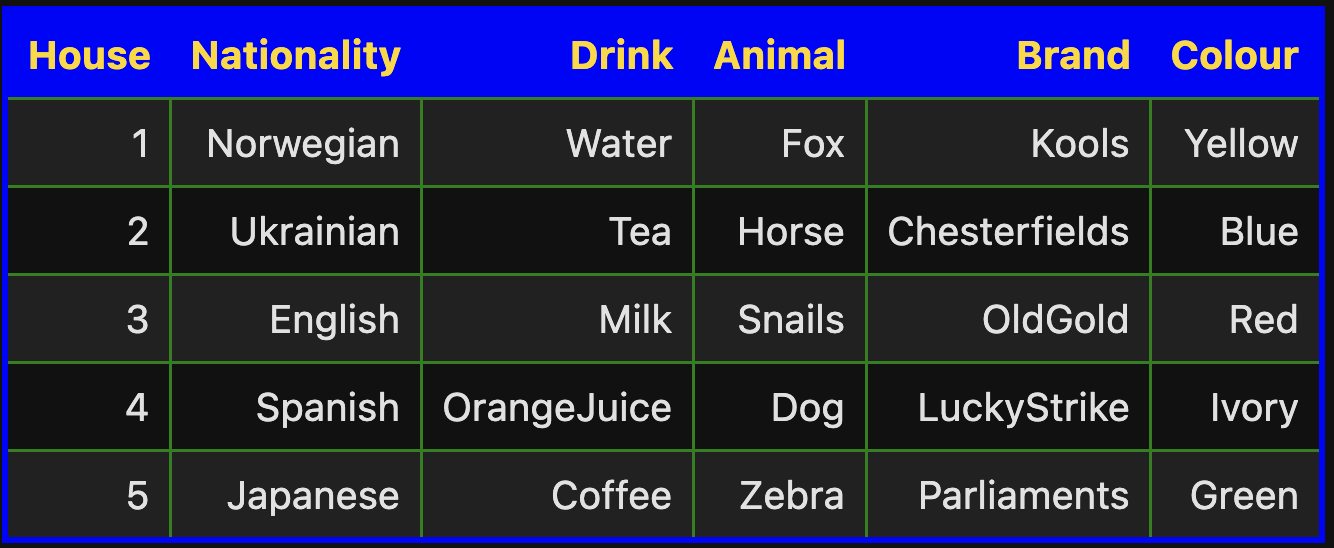
\epsfig{file=Figures/zebra.png, scale=0.7}} 
  \caption{The solution of the zebra puzzle.}
  \label{fig:zebra}
\end{figure}


\pagebreak

\FloatBarrier


\exerciseEng
Once upon a time, there was a king who wanted to marry his daughter to a
prince. He had it proclaimed throughout the land that he was seeking a husband
for his daughter. One day, a prince came by to apply for the position. 

Since the king did not want to marry his daughter to some dullard, he led the
prince into a room with nine doors. The king told the prince that the princess
was in one of the rooms, but that there were other rooms behind which hungry
tigers were waiting. Some rooms were also empty. If the prince opened a door
with a tiger behind it, it would probably be his last mistake. 

The king went on to say that there were signs on all the doors with statements on them. These statements behave as follows:
\begin{enumerate}
\item In the rooms where there is a tiger, the statement on the sign is false.
\item In the room where the princess is, the statement is true.
\item With regards to the the empty rooms, the situation is a bit more
      complicated, because there are two possibilities:
      \begin{itemize}
      \item Either all the inscriptions on the empty rooms are true,
      \item or all the inscriptions on the empty rooms are false.
      \end{itemize}

\end{enumerate}
The prince then read the inscriptions. These were as follows:
\begin{enumerate}
\item Room: The princess is in a room with an odd number and
      there is no tiger in the rooms with an even number.
\item Room: This room is empty.
\item Room: The inscription on Room No. 5 is true, the inscription on Room No. 7 is false,
      and there is a tiger in Room No. 3.
\item Room: The inscription on Room No. 1 is false, there is no tiger in Room No. 8,
      and the inscription on Room No. 9 is true.
\item Room: If the inscription on Room No. 2 or on Room No. 4 is true,
      then there is no tiger in Room No. 1.
\item Room: The inscription on Room No. 3 is false, the princess is in Room No. 2,
      and there is no tiger in Room No. 2.
\item Room: The princess is in Room No. 1 and the inscription on Room No. 5 is true.
\item Room: There is no tiger in this room and Room No. 9 is empty.
\item Room: Neither in this room nor in Room No. 1 is there a tiger, and moreover, the
      inscription on Room No. 6 is true.
\end{enumerate} 
I have provided the framework of a notebook at the following address:
\\[0.2cm]
\hspace*{1.3cm}
\href{https://github.com/karlstroetmann/Logic/blob/master/Python/Chapter-4/Prince-Tiger.ipynb}{\texttt{github.com/karlstroetmann/Logic/blob/master/Python/Chapter-4/Prince-Tiger.ipynb}}
\\[0.2cm]
You should edit this notebook in order to solve the given problem. \eox
\vspace*{1cm}

\exerciseEng
The following exercise is taken from the book 
\href{https://www.amazon.de/Logeleien-Zweistein-ihren-Antworten-Wegner/dp/B006YF0VUE}{99 Logeleien von Zweistein}.
This book has been published 1968.  It is written by 
\href{http://de.wikipedia.org/wiki/Thomas_von_Randow}{Thomas von Randow}.

\begin{minipage}{0.95\linewidth}
  {\sl
    The gentlemen \emph{Amann}, \emph{Bemann}, \emph{Cemann} and \emph{Demann} are called - not
    necessarily in the same order - by their 
    first names \emph{Erich}, \emph{Fritz}, \emph{Gustav} and \emph{Heiner}. They are all married to
    exactly one woman. We also know the following about them and their wives: 
    \begin{enumerate}
    \item Either \emph{Amann's} first name is \emph{Heiner}, or \emph{Bemann's} wife is \emph{Inge}.
    \item If \emph{Cemann} is married to \emph{Josefa}, then - \textbf{and only in this case} -
          \emph{Klara's} husband is \textbf{not} called \emph{Fritz}.
    \item If \emph{Josefa's} husband is \textbf{not} called \emph{Erich}, then \emph{Inge} is married to
          \emph{Fritz}. 
    \item If \emph{Luise's} husband is called \emph{Fritz}, then \emph{Klara's} husband's first name is
          \textbf{not} \emph{Gustav}. 
    \item If the wife of \emph{Fritz} is called \emph{Inge}, then \emph{Erich} is \textbf{not} married to
          \emph{Josefa}. 
    \item If \emph{Fritz} is \textbf{not} married to \emph{Luise}, then \emph{Gustav's} wife's name is \emph{Klara}.
    \item Either \emph{Demann} is married to \emph{Luise}, or \emph{Cemann} is called \emph{Gustav}.
    \end{enumerate}
    What are the full names of these gentlemen, and what are their wives' first names?}
\end{minipage}
\vspace*{0.3cm}

\noindent
I have provided the framework of a notebook at the following address:
\\[0.2cm]
\hspace*{1.3cm}
\href{https://github.com/karlstroetmann/Logic/blob/master/Python/Chapter-4/Zweistein.ipynb}{\texttt{github.com/karlstroetmann/Logic/blob/master/Python/Chapter-4/Zweistein.ipynb}}
\\[0.2cm]
You should edit this notebook in order to solve the given problem.

\pagebreak


\section{Check Your Comprehension}
\begin{enumerate}[(a)]
\item How have we defined the set of propositional logic formulas?
\item How have we defined the semantics of propositional logic formulas?
\item How do we represent propositional logic formulas in \textsl{Python}?
\item What is a tautology?
\item How can we transform propositional logic formula into conjunctive normal
      form?
\item How did we define the proof concept $M \vdash C$?
\item What are the most important properties of the proof concept $\vdash$?
\item How did we define the notion of a set of clauses being solvable?
\item Do you know how the algorithm of Davis and Putnam works?
\item Can you code a logical puzzle as a propositional formula?
\end{enumerate}


%\input{compact-barwise}

%%% Local Variables: 
%%% mode: latex
%%% TeX-master: "logic"
%%% End: 
